% !TeX program = lualatex
\documentclass{fict}

\usepackage{lmodern}
\usepackage{tabularx}
\usepackage{booktabs}
\usepackage{array}
\usepackage{float}
\usepackage{amssymb}
\usepackage{multirow}
\usepackage{xurl}


\addbibresource{references.bib}
% Municipal & Project-Specific Terms
\newacronym[description={Artificial Intelligence to Optimise Cleansing in Malta}]{AICOM}{AICOM}{Artificial Intelligence to Optimise Cleansing in Malta}
\newacronym[description={Cleansing and Maintenance Division}]{CMD}{CMD}{Cleansing and Maintenance Division}
\newacronym[description={Institute of Electrical and Electronics Engineers}]{IEEE}{IEEE}{Institute of Electrical and Electronics Engineers}
\newacronym[description={Sustainable Development Goal}]{SDG}{SDG}{Sustainable Development Goal}
\newacronym[description={Internet of Things}]{IoT}{IoT}{Internet of Things}

% AI, Computer Vision & NLP Fundamentals
\newacronym[description={Artificial Intelligence}]{AI}{AI}{artificial intelligence}
\newacronym[description={Computer Vision}]{CV}{CV}{computer vision}
\newacronym[description={Object Detection}]{OD}{OD}{object detection}
\newacronym[description={Vision-Language Model}]{VLM}{VLM}{vision-language model}
\newacronym[description={Vision Foundation Model}]{VFM}{VFM}{vision foundation model}
\newacronym[description={Foundation Model}]{FM}{FM}{foundation model}
\newacronym[description={Natural Language Processing}]{NLP}{NLP}{natural language processing}
\newacronym[description={General Data Protection Regulation}]{GDPR}{GDPR}{General Data Protection Regulation}
\newacronym[description={Municipal Solid Waste}]{MSW}{MSW}{municipal solid waste}
\newacronym[description={Traffic-Sign Recognition}]{TSR}{TSR}{traffic-sign recognition}
\newacronym[description={Zero-Shot Detection}]{ZSD}{ZSD}{zero-shot detection}

% Datasets & Data Processes
\newacronym[description={Unmanned Aerial Vehicle}]{UAV}{UAV}{Unmanned Aerial Vehicle}
\newacronym[description={Maltese Domestic Waste Dataset}]{MDWD}{MDWD}{Maltese Domestic Waste Dataset}
\newacronym[description={Maltese Traffic Sign Dataset}]{MTSD}{MTSD}{Maltese Traffic Sign Dataset}
\newacronym[description={Exploratory Data Analysis}]{EDA}{EDA}{exploratory data analysis}
\newacronym[description={Quality Assurance}]{QA}{QA}{quality assurance}
\newacronym[description={Red-Green-Blue-Depth}]{RGBD}{RGB-D}{red-green-blue-depth}

% Object Detection Architectures & Components
\newacronym[description={You Only Look Once}]{YOLO}{YOLO}{You Only Look Once}
\newacronym[description={Contrastive Language--Image Pre-training}]{CLIP}{CLIP}{Contrastive Language--Image Pre-training}
\newacronym[description={Convolutional Neural Network}]{CNN}{CNN}{convolutional neural network}
\newacronym[description={Common Objects in Context}]{COCO}{COCO}{Common Objects in Context}
\newacronym[description={Non-Maximum Suppression}]{NMS}{NMS}{non-maximum suppression}
\newacronym[description={Roboflow Detection Transformer}]{RF-DETR}{RF-DETR}{Roboflow Detection Transformer}
\newacronym[description={Segment Anything Model}]{SAM}{SAM}{Segment Anything Model}
\newacronym[description={Deep Learning}]{DL}{DL}{deep learning}
\newacronym[description={World Foundation Model}]{WFM}{WFM}{world foundation model}
\newacronym[description={Detection Transformer}]{DETR}{DETR}{Detection Transformer}
\newacronym[description={Real-Time Detection Transformer}]{RT-DETR}{RT-DETR}{Real-Time Detection Transformer}
\newacronym[description={Light-Weight Detection Transformer}]{LW-DETR}{LW-DETR}{Light-Weight Detection Transformer}
\newacronym[description={Region-based Convolutional Neural Network}]{R-CNN}{R-CNN}{region-based convolutional neural network}
\newacronym[description={Region Proposal Network}]{RPN}{RPN}{region proposal network}
\newacronym[description={Region of Interest}]{RoI}{RoI}{region of interest}
\newacronym[description={Single Shot MultiBox Detector}]{SSD}{SSD}{Single Shot MultiBox Detector}
\newacronym[description={Feature Pyramid Network}]{FPN}{FPN}{feature pyramid network}
\newacronym[description={Neural Architecture Search}]{NAS}{NAS}{neural architecture search}

% Representation Learning & Visual Backbones
\newacronym[description={Self-Distillation with No Labels}]{DINO}{DINO}{Self-Distillation, No Labels}
\newacronym[description={Video Joint Embedding Predictive Architecture}]{VJEPA}{V-JEPA}{Video Joint Embedding Predictive Architecture}
\newacronym[description={Convolutional Network for the Network Architecture Search}]{ConvNeXt}{ConvNeXt}{Convolutional Network for the Network Architecture Search}
\newacronym[description={Low-Rank Adaptation}]{LoRA}{LoRA}{low-rank adaptation}
\newacronym[description={Vision Transformer}]{VIT}{ViT}{vision transformer}

% Evaluation Metrics
\newacronym[description={True Positive}]{TP}{TP}{true positive}
\newacronym[description={Average Precision}]{AP}{AP}{average precision}
\newacronym[description={Precision--Recall}]{PR}{PR}{precision--recall}
\newacronym[description={Mean Average Precision}]{mAP}{mAP}{mean average precision}
\newacronym[description={Intersection over Union}]{IoU}{IoU}{intersection over union}
\newacronym[description={Ground Truth}]{GT}{GT}{ground truth}
\newacronym[description={False Positive}]{FP}{FP}{false positive}
\newacronym[description={False Negative}]{FN}{FN}{false negative}

% Training & Optimisation
\newacronym[description={Fine-Tuning}]{FT}{FT}{fine-tuning}
\newacronym[description={Parameter-Efficient Fine-Tuning}]{PEFT}{PEFT}{parameter-efficient fine-tuning}
\newacronym[description={Brain Floating Point 16}]{BF16}{BF16}{brain floating point 16}
\newacronym[description={Half-Precision Floating Point 16}]{FP16}{FP16}{half-precision floating point 16}
\newacronym[description={Exponential Moving Average}]{EMA}{EMA}{exponential moving average}
\newacronym[description={Muon--Stochastic Gradient Descent hybrid optimiser}]{MuSGD}{MuSGD}{Muon--stochastic gradient descent}

% Hardware, Software & Systems
\newacronym[description={Compute Unified Device Architecture}]{CUDA}{CUDA}{Compute Unified Device Architecture}
\newacronym[description={CUDA Deep Neural Network Library}]{CUDNN}{cuDNN}{CUDA deep neural network library}
\newacronym[description={Central Processing Unit}]{CPU}{CPU}{central processing unit}
\newacronym[description={Graphics Processing Unit}]{GPU}{GPU}{graphics processing unit}
\newacronym[description={Double Data Rate 5}]{DDR5}{DDR5}{double data rate 5}
\newacronym[description={Random Access Memory}]{RAM}{RAM}{random access memory}
\newacronym[description={Video Random-Access Memory}]{VRAM}{VRAM}{video random-access memory}
\newacronym[description={Global Positioning System}]{GPS}{GPS}{Global Positioning System}
\newacronym[description={User Interface}]{UI}{UI}{user interface}
\newacronym[description={Quick-Response}]{QR}{QR}{quick-response}
\newacronym[description={JavaScript Object Notation}]{JSON}{JSON}{JavaScript Object Notation}

\title{A Comparative Study of Vision-Based\\Perception Paradigms for Urban Waste\\and Infrastructure Monitoring}
\author{Andrea Filiberto Lucas}
\supervisor{Dr Dylan Seychell}
\cosupervisor{Dr Mark Bugeja}
\degreename{M.Sc. in Artificial Intelligence}
\titledate{September 2026}

\begin{document}

\frontmatter{}
\pagestyle{pageNumbersOnly}

\makeatletter
\begin{titlepage}
    \begin{flushleft}
        \begin{minipage}[t][5.2cm][t]{\textwidth}
            \begin{Huge}
                \textbf{\@title}
            \end{Huge}
        \end{minipage}
        %
        \begin{minipage}[t][1.3cm][t]{\textwidth}
            \begin{LARGE}
                \textbf{\@author}
            \end{LARGE}
        \end{minipage}
        %
        \begin{minipage}[t][3.9cm][t]{\textwidth}
            \begin{Large}
                \begin{tabular}{@{}ll@{}}
                    Supervisor:    & \@supervisor{}   \\
                    \ifdefined\@cosupervisor{}%
                    Co-Supervisor: & \@cosupervisor{} \\
                    \fi%
                \end{tabular}
            \end{Large}
        \end{minipage}
        %
        \begin{minipage}[t][9.5cm][t]{\textwidth}
            \begin{Large}
                \@titledate{}
            \end{Large}
        \end{minipage}
        %
        \begin{large}
            \textit{Submitted in partial fulfilment of the requirements}
            \newline
            \textit{for the degree of \@degreename{}.}
        \end{large}

        \vfill

        
\includegraphics[width=9.4cm,keepaspectratio]{figures/ict_logo}
    \end{flushleft}
\end{titlepage}
\makeatother

\chapter*{Abstract}
\addcontentsline{toc}{chapter}{Abstract}

[TODO: ADD ABSTRACT HERE]

\noindent\rule{\linewidth}{0.3pt}
\chapter*{Acknowledgements}
\addcontentsline{toc}{chapter}{Acknowledgements}

The research presented in this dissertation was funded by the \href{https://mdia.gov.mt/services/pathfinder-digital-scholarship/}
{Pathfinder Digital Scholarship}\footnote{\url{https://mdia.gov.mt/services/pathfinder-digital-scholarship/}}, awarded by the \href{https://mdia.gov.mt/}{Malta Digital Innovation Authority (MDIA)} under the 2025 call. The research was also closely motivated by the practical requirements of the \gls{AICOM} project, with key aspects of the work, including the development of the \gls{MDWD}, directly supporting its objectives and operational needs. The \gls{AICOM} project was funded by the Government of Malta's \href{https://publiccleanliness.gov.mt/public-bodies/cmd/}{Cleansing and Maintenance Division (CMD)}.\\\\

\noindent I would first like to thank my parents, Ian and Alexandra Lucas, for their patience, encouragement, and unwavering support throughout my Master's studies. Their confidence in me has been a constant source of motivation during the more demanding stages of this work and has been fundamental to my academic and personal development alike.\\

\noindent I wish to express my sincere gratitude to my supervisor and principal investigator, Dr Dylan Seychell, for his guidance and leadership throughout this dissertation. His technical insight, constructive feedback, and mentorship played a central role in shaping this work. I am equally grateful to my co-supervisor, Dr Mark Bugeja, for his considered advice and attentive reading of this work as it developed. His feedback helped refine both the research and its overall direction.\\

\noindent Finally, I would like to thank my colleagues and friends at the \href{https://www.um.edu.mt/research/dawl/}{Dawl AI Lab}, within the Department of Artificial Intelligence at the University of Malta, for their encouragement and companionship throughout this period.

\noindent\rule{\linewidth}{0.3pt}
\clearpage{}

\tableofcontents{}
\addcontentsline{toc}{chapter}{Contents}
\clearpage{}

\listoffigures{}
\addcontentsline{toc}{chapter}{List of Figures}
\clearpage{}

\listoftables{}
\addcontentsline{toc}{chapter}{List of Tables}
\clearpage{}

\printglossary[type=\acronymtype,nonumberlist,title=List of Abbreviations]
\addcontentsline{toc}{chapter}{List of Abbreviations}
\noindent\rule{\linewidth}{0.3pt}
\clearpage{}

\mainmatter{}
\pagestyle{MainMatter}

\glsresetall
\chapter{Introduction}
\label{ch:introduction}
\glsresetall
This introductory chapter situates the dissertation within the broader context of municipal monitoring in Malta, establishing the practical problem and the technical motivations for an automated perception approach suited to the local setting. It subsequently introduces the comparative study undertaken, states the principal aim and objectives of this dissertation, and outlines the structure of the remaining chapters.

\section{Problem Definition}
\label{sec:problem-definition}
Municipal services depend on the timely identification of conditions requiring cleansing, maintenance or further inspection, including accumulated or incorrectly presented waste and deteriorated roadside infrastructure \cite{I1,I2,I3,I4}. In practice, this information is still obtained largely through manual inspections, periodic patrols and reports submitted by members of the public \cite{BG1-repeatedinspection,BG4-human-inspection,BG2-waste-reporting}. Although these mechanisms provide valuable local knowledge, their spatial and temporal coverage is inherently limited, while the frequency and distribution of citizen reports do not necessarily reflect the conditions present across different localities \cite{BG3-citizen-reporting,BG6-reporting-bias}. Maintaining consistent observation across extensive road networks and multiple municipal areas therefore remains an operational challenge \cite{urbanproblem,BG7-driveby-sensing}.

Street-level imagery offers a means of extending observational coverage and supporting the automated or assisted assessment of conditions across the road network \cite{ashraf2026urbaninfrastructure}. However, the Maltese streetscape presents a challenging visual environment, characterised by dense urban development, restricted street space and considerable variation in both object appearance and image acquisition conditions \cite{I5-malta,I6-malta,BG15-mdwd}. Consequently, automated methods should be evaluated under conditions representative of this setting, rather than assessed solely through performance reported on datasets originating from different geographic and operational contexts. Within this context, the dissertation addresses two related applications: the detection and categorisation of kerbside \gls{MSW}, and the recognition of traffic signs and associated roadside infrastructure. The latter extends beyond object localisation to the assessment of visible characteristics relevant to infrastructure monitoring and maintenance \cite{BG5-sign-monitoring,BG29-sign-inspection,BG30-sign-visual-condition}. While both applications rely on the interpretation of street-level imagery, they differ in their visual characteristics, operational significance and downstream requirements.

Given these differing task characteristics, several contemporary \gls{CV} paradigms merit consideration, including supervised \gls{OD}, zero-shot prompt-based localisation and attribute classification using pretrained visual representations \cite{BG33-object-detection,I9,BG37-open-vocabulary,BG41-visual-attributes}. These paradigms vary in supervision requirements, output structure and adaptability to new categories or conditions.

\noindent This dissertation therefore asks not whether municipal objects can be recognised in Maltese street-level imagery, but which perception paradigm best balances predictive performance, robustness, computational cost and practical applicability for each localisation task, and which transfer strategy most effectively exploits pretrained visual representations for characterising traffic-sign infrastructure.

\section{Motivation}
\label{sec:motivation}
The case for improved municipal monitoring rests on the need for more timely and consistent evidence regarding conditions affecting public spaces and roadside infrastructure. Reliable waste collection and the maintenance of clean streets contribute to public health and environmental quality \cite{BG8-waste-impacts}, while visible and serviceable traffic-sign infrastructure supports the safe use of the road network \cite{BG5-sign-monitoring}.These objectives also align with \gls{SDG}~11, whose targets include reducing the environmental impact of cities, improving waste management, and providing safe, accessible transport \cite{un2015sdgs}. Increasing the spatial and temporal coverage of observation could therefore support more informed maintenance and operational decision-making \cite{kumar2026gvp}. Automated visual analysis, in this context, is intended to complement rather than replace human judgement, reducing the volume of imagery requiring manual review and directing attention towards locations more likely to require intervention.

Nonetheless, existing \gls{CV} research does not fully capture the characteristics of the two Maltese monitoring domains considered in this dissertation. Waste-recognition studies commonly focus on isolated objects, material sorting or litter detection, rather than the kerbside presentation and collection-stream categories used in Malta \cite{bartolo2026aeriallitter,proenca2020taco,MJU-Waste}. Traffic-sign detection and recognition are considerably more established research areas, supported by large benchmark datasets \cite{houben2013gtsdb, stallkamp2012gtsrb, ertler2020mapillary,katsamenis2025dorie}. However, these benchmarks primarily focus on sign detection and semantic classification, with comparatively limited representation of visual and physical characteristics relevant to infrastructure monitoring and maintenance.

In parallel, the technical landscape has expanded beyond conventional supervised \gls{OD} to include prompt-based localisation, \glspl{VLM} and large pretrained visual encoders suited to diverse adaptation strategies \cite{kirillov2023segment,meta2025sam3,simeoni2025dinov3,hu2022lora}. Yet reported results typically derive from differing datasets, resolutions, hardware and evaluation protocols, hindering direct comparison. The literature reviewed here does not establish how these paradigms compare on the two Maltese monitoring tasks under a shared, task-appropriate evaluation framework. Establishing the relative strengths and limitations of supervised detection, zero-shot localisation and pretrained visual representations within their respective locally defined tasks is therefore the principal motivation for this dissertation.

\newpage
\section{Research Approach}
\label{sec:research-approach}
To address the problem established above, this dissertation adopts a comparative experimental approach across two municipal-monitoring domains using two purpose-built Maltese datasets. The \textbf{\gls{MDWD}} contains street-level imagery of kerbside domestic waste annotated for \gls{OD} \cite{BG15-mdwd}, while the \textbf{\gls{MTSD}} comprises traffic signs and associated roadside infrastructure annotated at object level with attributes relevant to infrastructure monitoring. Although representing different municipal tasks, both datasets originate from Maltese street-level environments, providing a common local setting for investigating different \gls{CV} approaches.

\begin{figure}[htbp]
    \centering
    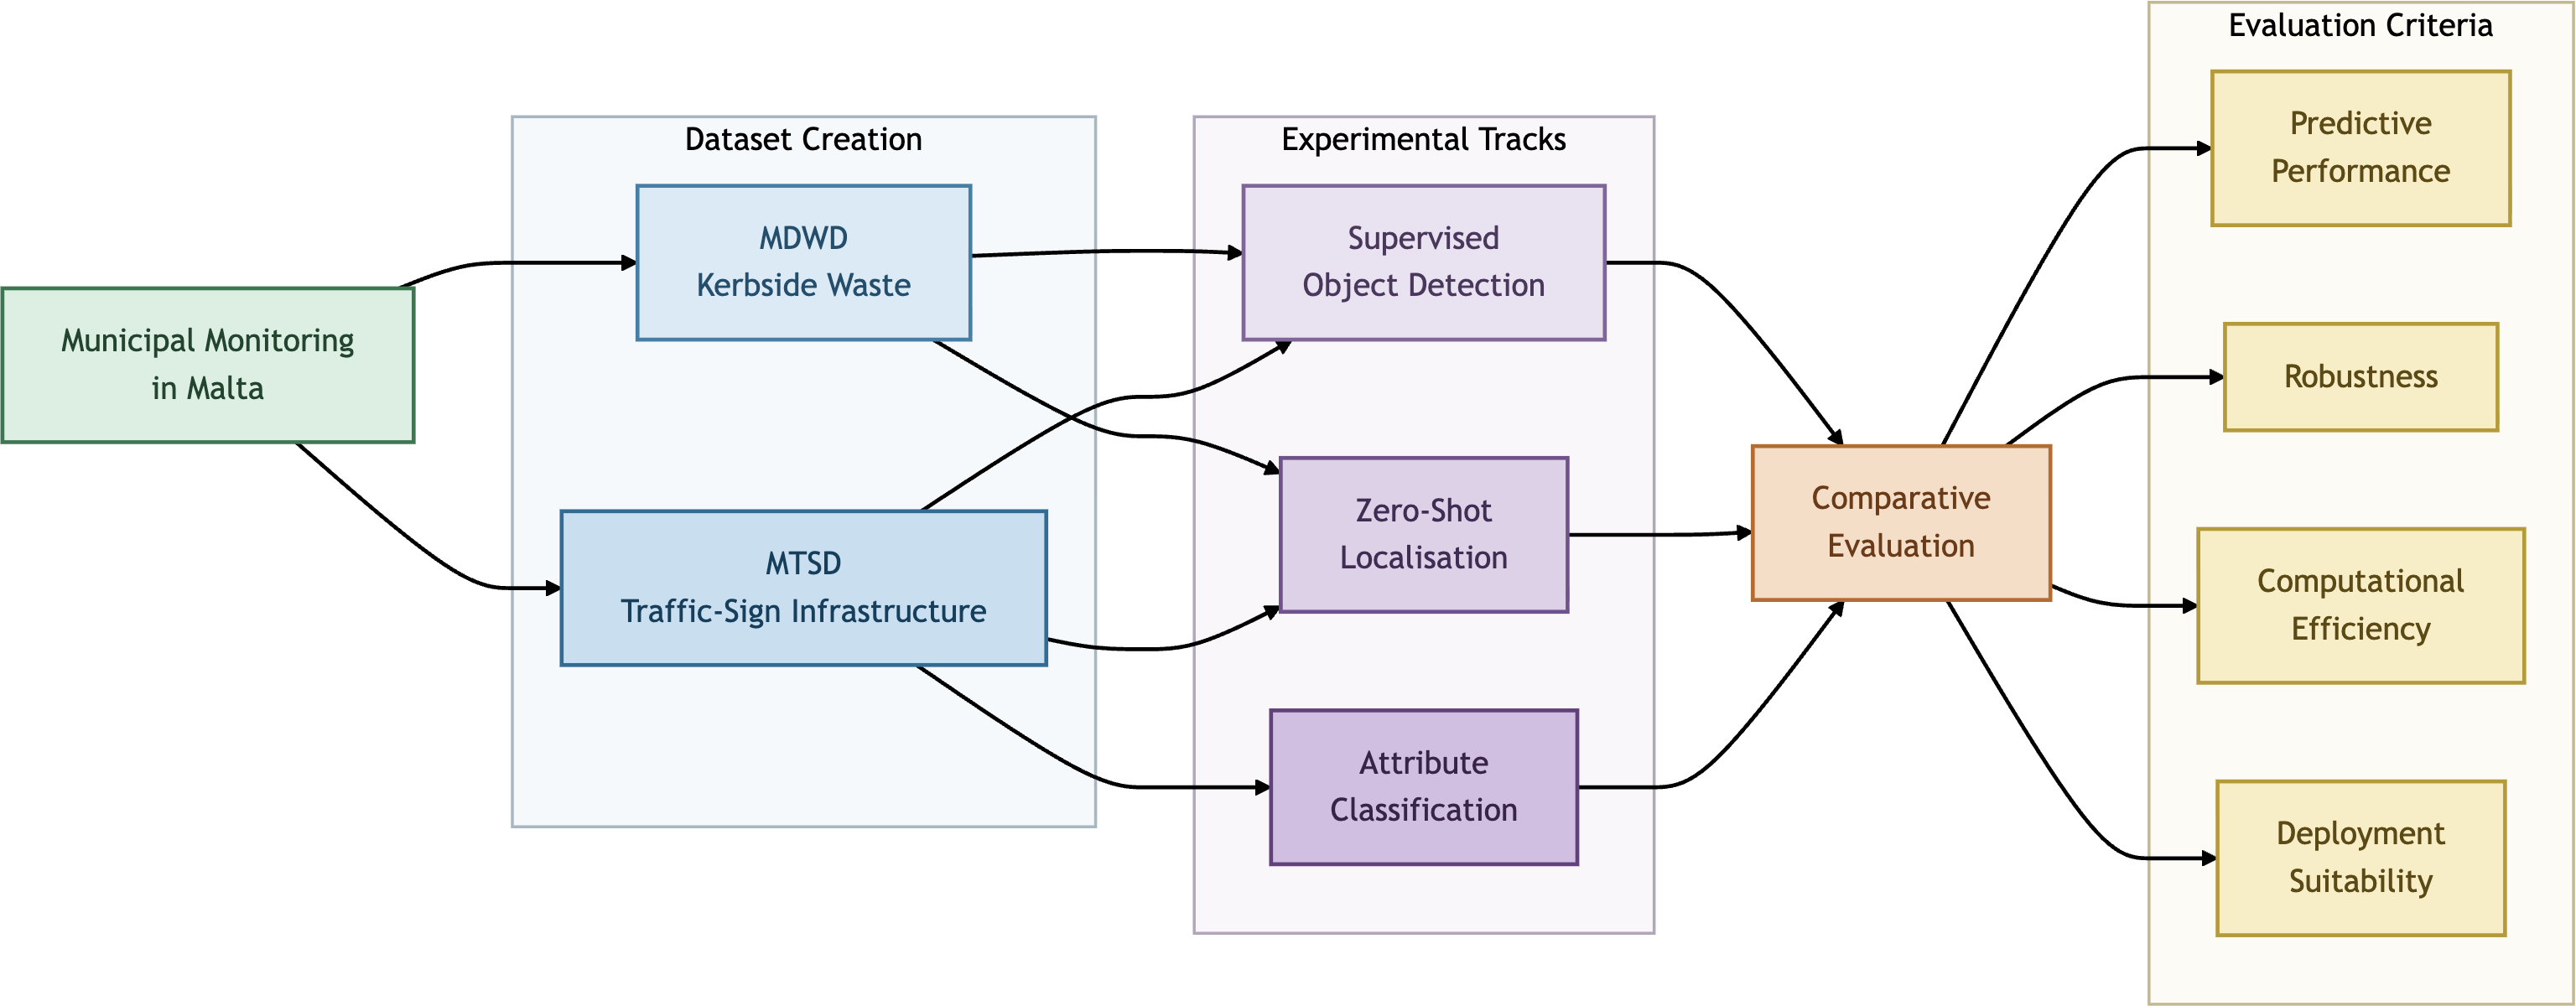
\includegraphics[width=\textwidth]{figures/ResearchApproach.png}
    \caption{Overview of the research approach, showing the relationship between the Maltese municipal-monitoring datasets, experimental tracks and comparative evaluation criteria.}
    \label{fig:research-approach}
\end{figure}

\noindent The empirical study is organised into three complementary experimental tracks, as illustrated in Figure~\ref{fig:research-approach}. The first investigates supervised \gls{OD} across both datasets, comparing \gls{YOLO}-family detectors with a detection-transformer architecture under a common evaluation procedure. The second evaluates zero-shot object localisation using promptable localisation models and grounded \glspl{VLM}, applied without task-specific parameter optimisation and assessed against the same held-out \gls{GT} annotations. The third examines traffic-sign attribute classification using \gls{GT} object crops from the \gls{MTSD}. Pretrained visual representations are compared within a shared multi-head classification framework using frozen feature extraction, parameter-efficient adaptation and, where computationally feasible, full \gls{FT} to assess viewing angle, mounting type, physical condition and geometric shape.

Across the three tracks, evaluation considers predictive performance, robustness, computational efficiency and practical deployment suitability. The resulting framework therefore examines not only model performance, but also the trade-offs between perception paradigms and their suitability for the municipal-monitoring tasks considered.

\section{Aims and Objectives}
\label{sec:aims-objectives}
The primary aim of this dissertation is to evaluate the suitability of contemporary vision-based perception paradigms and transfer strategies for kerbside-waste and traffic-sign infrastructure monitoring in Malta. This aim is addressed through the following objectives:

\begin{enumerate}
    \item \textbf{Construct and characterise two Malta-specific street-level datasets}, by defining their taxonomies and annotation criteria, coordinating image acquisition and professional annotation, and quality-assuring the resulting \gls{MDWD} for kerbside \gls{MSW} detection and the \gls{MTSD} for traffic-sign infrastructure monitoring. Both provide verified object-level annotations, with \gls{MTSD} instances additionally annotated for viewing angle, mounting type, physical condition and geometric shape.
    
    \item \textbf{Train and comparatively evaluate supervised detectors}, by training \gls{YOLO}11, \gls{YOLO}\\12, \gls{YOLO}26 and \gls{RF-DETR} on both datasets within a shared experimental framework, with framework-specific training differences recorded explicitly. Performance is quantified using detection, robustness and computational-efficiency measures, with controlled \gls{MTSD} experiments additionally assessing the effects of model scale, data augmentation and input resolution.

    \item \textbf{Quantify the effectiveness of zero-shot object localisation}, by evaluating \gls{SAM}~3, \gls{SAM}~3.1, LocateAnything and Cosmos Reason2 against common held-out \gls{GT} annotations without task-specific parameter optimisation. Localisation performance, sensitivity to prompt formulation and per-image inference cost are quantified, using controlled prompt variants where applicable, and compared with supervised \gls{OD}.
     
    \item \textbf{Compare transfer strategies for traffic-sign attribute classification}, by evaluating frozen feature extraction, \gls{LoRA}-based adaptation and full \gls{FT}, where computationally feasible, across \gls{DINO}v3, \gls{VJEPA}~2.1, ConvNeXt and LingBot-Vision within a common multi-head classification framework. Performance and computational requirements are quantified across viewing angle, mounting type, physical condition and geometric shape to identify the most effective representation--transfer strategy combinations for the \gls{MTSD}.

\end{enumerate}

\newpage
\noindent The conclusions drawn from these objectives are restricted to the two Maltese monitoring domains and datasets considered in this dissertation. Differences in dataset coverage, model characteristics and experimental conditions are therefore explicitly considered when interpreting the results, rather than treating the findings as universal comparisons between the underlying model families.

\section{Document Structure}
\label{sec:document-structure}
The remainder of this dissertation is organised into four chapters: \medskip

\noindent \textbf{\hyperref[ch:bg-lit]{Chapter 2 -- Background and Literature Review}} establishes the municipal and technical context of the study. It introduces the Maltese monitoring setting and the datasets used in this research, before reviewing related work and the \gls{CV} approaches relevant to the three experimental tracks. \medskip

\noindent \textbf{\hyperref[ch:methodology]{Chapter 3 -- Methodology}} describes the experimental framework and dataset preparation, together with the methods used for supervised detection, zero-shot localisation and traffic-sign attribute classification. \medskip

\noindent \textbf{\hyperref[ch:evaluation]{Chapter 4 -- Evaluation}} presents and analyses the experimental results, comparing the investigated approaches across the established evaluation dimensions and examining their principal failure modes. \medskip

\noindent \textbf{\hyperref[ch:conclusion]{Chapter 5 -- Conclusion}} consolidates the findings in relation to the dissertation aims and objectives, summarises the principal contributions and limitations, and identifies directions for future research.

\noindent\rule{\linewidth}{0.3pt}
\chapter{Background and Literature Review}
\label{ch:bg-lit}
This chapter establishes the municipal, empirical and technical foundations of the dissertation. It first defines municipal visual monitoring in the Maltese context and introduces the \gls{MDWD} and \gls{MTSD}, comparing them with related datasets in the literature. It then reviews the \gls{CV} tasks and model paradigms used in the empirical work, before concluding with the deployment and evaluation concepts relevant to the study.

\section{Municipal Visual Monitoring}
\label{sec:bg-municipal}
Municipal visual monitoring refers to the repeated observation of public spaces and infrastructure in order to identify conditions that may require cleansing, maintenance or further attention \cite{torneiro2025urbanmonitoring}. This formulation underpins both kerbside waste and roadside infrastructure as monitoring domains, and is shaped in turn by the characteristics of the Maltese setting in which it is applied.

\subsection{Municipal Monitoring and Visual Observation}
\label{sec:bg-municipal-inspection}
Municipal monitoring conventionally relies on observations of the physical environment, obtained through routine inspections by municipal personnel and reports submitted by members of the public \cite{BG1-repeatedinspection,BG2-waste-reporting,BG3-citizen-reporting}. Human assessment remains important, since the significance of an observed condition often depends on contextual and operational knowledge that extends beyond its visual appearance \cite{BG4-human-inspection}. Automated visual monitoring is accordingly treated here as a means of supporting existing inspection and reporting practice, extending its coverage rather than substituting for the contextual judgement on which operational decisions depend.

Within this dissertation, a municipal visual observation is understood to accumulate information across successive stages. An object of interest is first identified within the streetscape and spatially localised, after which it is characterised according to properties relevant to the corresponding municipal service. Where imagery is associated with geographical position, the resulting observation can additionally be linked to the location at which the condition was encountered, giving it both a description and a place within the road network.

Opportunistically captured imagery, gathered during journeys undertaken for other purposes, extends observation beyond dedicated inspection activity and increases the spatial frequency at which municipal conditions are encountered \cite{BG7-driveby-sensing,BG10-vehicle-sensing}. Such imagery can be processed automatically, with selected observations flagged for review so that subsequent inspection effort is concentrated where conditions are more likely to warrant it.

\subsection{Waste and Road Infrastructure as Monitoring Domains}
\label{sec:bg-monitoring-domains}
As established in Section~\ref{sec:problem-definition}, this dissertation considers two municipal monitoring domains, namely kerbside domestic waste and traffic-sign infrastructure, whose operational characteristics differ substantially. Waste represents a comparatively transient condition whose presence, presentation and relevance may change between successive collection cycles \cite{wastecollection2026web,era2023web}, whereas traffic signs and related roadside infrastructure are persistent physical assets whose state changes more gradually through ageing, damage and environmental exposure \cite{BG14-sign-degradation,BG5-sign-monitoring}. Despite this distinction, both can be expressed through a common visual-monitoring formulation in which relevant objects are first localised within street-level imagery and subsequently characterised using information meaningful to the responsible service.

For kerbside waste, characterisation extends beyond establishing that discarded material is present. Waste encountered within the streetscape may include standard collection bags, loose discarded objects, bulky items and material associated with \gls{CMD}'s cleansing activities \cite{BG15-mdwd,wasteserv2026web}. Its interpretation depends partly on presentation, since the Maltese collection system associates different domestic waste streams with designated formats and collection schedules \cite{wastecollection2026web,era2023web}. Distinguishing these visually observable streams therefore provides information a single generic waste category would not capture, motivating the categories defined for the \gls{MDWD} in Subsection~\ref{sec:bg-mdwd}.

Road-infrastructure monitoring similarly extends beyond recognising the semantic category of a traffic sign. Conventional sign recognition is principally concerned with recovering the regulatory or informational meaning conveyed by the sign face, whereas infrastructure monitoring is also concerned with the physical asset through which that meaning is displayed. Properties such as mounting configuration, viewing orientation and visible physical condition therefore remain relevant even when semantic identity is uncertain \cite{BG16-malta-sign-guidelines,BG16-eu-rism,BG29-sign-inspection}. Deterioration, including fading, surface damage and loss of visibility, may affect whether an asset requires inspection or maintenance \cite{BG14-sign-degradation,BG5-sign-monitoring}, and a rear-facing or otherwise unidentifiable sign can likewise remain a useful infrastructure observation even when its meaning cannot be recovered from the available image. These requirements motivate the object and attribute taxonomy adopted for the \gls{MTSD}, described in Subsection~\ref{sec:bg-mtsd}.

The two domains therefore diverge in what gives an observation its significance: the transient presentation of waste, as against the persistent identity, installation and physical state of infrastructure. In both cases, however, localisation alone provides an incomplete observation. It is the combination of location and domain-specific characterisation that forms the common basis for the two monitoring problems considered in this dissertation.

\subsection{The Maltese Streetscape and Monitoring Environment}
\label{sec:bg-malta}
Both monitoring domains are additionally shaped by the environment in which they are observed. Malta combines high population density and extensive urban development within a small and strongly car-dependent island state, where limited street space is divided between vehicular movement, parking, pedestrians, building frontages and roadside infrastructure \cite{I5-malta,I6-malta,BG19-malta-slow-streets}. Many localities contain narrow streets and pavements together with substantial on-street parking, restricting sightlines towards objects positioned close to the kerb and increasing the likelihood of partial occlusion by vehicles and surrounding street furniture \cite{BG18-malta-walkability,BG15-mdwd}.

Each domain introduces its own locally specific source of visual variation. Domestic waste streams are collected through a national door-to-door system in which waste is placed at the kerbside in designated colour-coded bags on scheduled collection days, appearing directly within the public streetscape, commonly at pavement or kerb level and alongside parked vehicles and other visually competing objects \cite{wastecollection2026web,era2023web,BG15-mdwd}. Colour and presentation therefore provide visually observable information directly related to the collection system within which waste is encountered. Traffic-sign infrastructure, by contrast, is shaped primarily by structural rather than presentational differences. Maltese specifications for permanent roadside signs encompass multiple configurations and requirements for sign plates, retro-reflective materials, supporting structures and mounting hardware \cite{infrastructuremalta2020spec}, so that roadside assets vary in semantic function, geometric form, orientation and mounting configuration, often positioned close to buildings, boundary walls and utility poles within a constrained streetscape.

Image acquisition and environmental exposure introduce additional sources of inconsistency. Street-level imagery may exhibit substantial contrast between direct sunlight and shadow, glare can obscure otherwise visible sign surfaces, and movement of the capturing platform can introduce blur \cite{BG15-mdwd,BG20-sign-glare}. Malta's marine environment is also significant over the longer term, since exposure to marine atmospheres can accelerate corrosion of metallic components, while traffic-sign retro-reflectivity and surface condition deteriorate progressively through service life \cite{BG21-marine-corrosion,BG14-sign-degradation}. This deterioration occurs along a continuum rather than as an immediate transition between an intact and failed state, supporting the use of ordered visual categories to describe physical condition \cite{BG22-sign-condition}. These characteristics collectively motivate the use of locally representative imagery when evaluating municipal visual monitoring within the Maltese streetscape.

\newpage
\subsection{Governance and Operational Responsibility}
\label{sec:bg-governance}
These environmental and structural characteristics are compounded by the distribution of institutional responsibility for the two domains across several Maltese public bodies. Kerbside domestic waste collection is organised through local and regional councils under the national collection framework, WasteServ Malta operates downstream treatment and disposal facilities, and the \gls{CMD} handles public cleansing and the removal of illegally deposited waste \cite{wastecollection2026web,era2023web,wasteserv2026web,cmd2026web}. Transport Malta provides national transport regulation and traffic-sign guidance, Infrastructure Malta develops and maintains substantial parts of the road network, and local councils retain authority over roads and public spaces within their respective localities \cite{transportmalta2021guidelines,infrastructuremalta2020spec,localcouncilsact1993}.

This distribution gives geographical position a further operational role beyond that already established for object identity and condition, since the appropriate destination of an observation can depend on where it was captured as much as what it describes. Within the Maltese setting, this reinforces the case for locally representative data and for the richer, object-level descriptions adopted by the two datasets introduced in Section~\ref{sec:bg-datasets}.

\section{Datasets and Annotation Taxonomies}
\label{sec:bg-datasets}
The two monitoring domains established in Subsection~\ref{sec:bg-monitoring-domains} are represented through two purpose-built Maltese datasets, whose object categories and attributes define the corresponding municipal observations as annotated \gls{CV} tasks. The \gls{MDWD} describes kerbside domestic waste primarily through visible presentation, while the \gls{MTSD} combines roadside-asset categories with object-level attributes describing viewing angle, mounting type, physical condition and geometric shape. Their construction, annotation procedures and \gls{EDA} are detailed in Section~\ref{sec:md-dataset-construction}.

\glsreset{MDWD}
\glsreset{MTSD}
\subsection{\gls{MDWD}}
\label{sec:bg-mdwd}
The \gls{MDWD} is a street-level \gls{OD} dataset developed to represent \gls{MSW} as it is visually encountered within the Maltese streetscape \cite{BG15-mdwd}. Its five object classes distinguish the principal bag-based streams of the national kerbside collection system from waste associated with public cleansing and other forms of waste that fall outside these streams \cite{BG15-mdwd,wastecollection2026web}. The taxonomy is based on characteristics that can be determined from road-facing imagery, primarily presentation, colour, form and context, rather than on the underlying material composition of an object. This is necessary because the contents of sealed or opaque refuse bags cannot be determined visually, and assigning labels based on information unavailable in the image would introduce systematic annotation uncertainty.

\subsubsection{Waste Terminology and Annotation Scope}
\label{sec:bg-waste-term}
The terminology used for waste requires separating the physical object being observed from the circumstances under which it entered the streetscape. In its broadest sense, \emph{waste} follows the definition established by the European Union Waste Framework Directive as a substance or object that its holder discards, intends to discard, or is required to discard \cite{BG23-waste-framework}. Within this category, \emph{kerbside-presented \gls{MSW}} is used throughout this dissertation for domestic waste intentionally placed for collection under the established national schedule \cite{wastecollection2026web}.

\emph{Litter} instead refers to loose waste whose visible presentation is consistent with material having been dropped, left or deposited in a public place rather than presented for scheduled collection. This follows the distinction in Maltese legislation between litter deposited in public spaces and refuse lawfully presented for collection \cite{BG24-malta-litter}. A related but separate category, \emph{bulky waste}, describes large discarded objects such as furniture, mattresses and household appliances \cite{BG25-bulky-waste}. By contrast, \emph{illegal dumping} describes the circumstances and legality of disposal rather than a category defined by visual appearance \cite{BG26-illegal-disposal}.

What separates kerbside-presented waste, litter and illegal dumping from one another is therefore largely a matter of intent and legality rather than appearance: a black bag placed at the kerb on collection day and one dumped illegally elsewhere may be visually indistinguishable, yet correspond to entirely different operational categories. Bulky waste, by contrast, is defined by the physical form of the object itself, and may co-occur with any of these circumstances. As intent, legality and circumstance cannot reliably be recovered from an image, the taxonomy set out below instead classifies instances according to the collection stream that their presentation most plausibly indicates, rather than by the terminology introduced above.

\subsubsection{Object-Class Taxonomy}
\label{sec:bg-mdwd-taxonomy}
The five \gls{MDWD} classes are summarised in Table~\ref{tab:mdwd-taxonomy}. For the principal streams, the operational meaning of each class is defined by the national collection scheme \cite{wastecollection2026web,era2023web}, while annotation follows the bag type visible within the image.

\begin{table}[H]
\centering
\caption{Object classes and annotation basis of the \gls{MDWD}.}
\label{tab:mdwd-taxonomy}
\begin{tabularx}{\textwidth}{@{}p{2.9cm} p{4.1cm} X@{}}
\toprule
\textbf{Class} & \textbf{Typical Visual\newline Presentation} & \textbf{Associated Collection Stream} \\
\midrule

    Mixed Waste
    & Black refuse bags
    & Non-separable household waste comprising soiled or composite packaging, sanitary products, household sweepings, ceramics and worn textiles, with hazardous and electrical items excluded from the stream. \\

    \addlinespace[0.5em]

    Recyclable\newline Material
    & Grey or green refuse bags
    & Co-mingled recyclable household stream comprising accepted paper, cardboard, metal and plastic packaging. \\

    \addlinespace[0.5em]

    Organic Waste
    & White or transparent refuse bags
    & Biodegradable household stream comprising food scraps, flowers, leaves and other accepted kitchen waste presented for organic collection. \\

    \addlinespace[0.5em]

    Orange \gls{CMD}
    & Orange refuse bags
    & Waste associated with \gls{CMD} street-cleansing activity rather than a household separation stream. \\

    \addlinespace[0.5em]

    Other Waste
    & No single designated presentation
    & Waste outside the four preceding bag-based categories, including bulky objects, loose discarded material, glass presented separately, flattened cardboard and open containers. \\

\bottomrule
\end{tabularx}
\end{table}

\noindent A consequence of this bag-based taxonomy is that material is classified as \emph{Recyclable Material} only when presented in the designated bag. Loose or non-standard recyclable items, such as flattened cardboard, are instead assigned to \emph{Other Waste}. The taxonomy therefore reflects the visually identifiable collection stream rather than the recyclability of the material itself. The same principle applies to \emph{Orange \gls{CMD}} bags: their typical contents, including street sweepings, vegetation and debris collected during cleansing operations \cite{cmd2026web}, are not annotated as waste when encountered loose, so recognition depends on the presence of the bag. Consequently, \emph{Other Waste} serves as a residual, exclusion-based category and is visually more heterogeneous than the designated bag-based streams. It is retained, however, to avoid assigning objects to categories unsupported by their visible presentation. Ambiguity remains where illumination, soiling, overlap or occlusion obscures these visual cues, particularly among closely grouped bags and objects within this heterogeneous class.

\subsection{\gls{MTSD}}
\label{sec:bg-mtsd}
The \gls{MTSD} is a street-level dataset of Maltese traffic signs and related roadside infrastructure developed to support both \gls{OD} and object-level attribute classification. Each annotated instance is localised by a bounding box, assigned to one of twelve object classes, and described through four object-level attributes, detailed in Subsection~\ref{sec:bg-attributes}. The taxonomy is operational rather than exhaustive, representing the roadside assets selected for monitoring rather than attempting to reproduce the complete catalogue of signs used in Malta.

Private notices, advertisements and other signage outside the monitoring scope are excluded, while roadside infrastructure relevant to sightlines or road operation is retained even where it is not a conventional traffic sign. This includes convex mirrors and directional bollards, both recognised by Transport Malta as means of improving visibility and guiding road users where sight distance or alignment is otherwise inadequate \cite{BG27-malta-road-mirrors}.

\subsubsection{Object-Class Taxonomy}
\label{sec:bg-mtsd-taxonomy}
The twelve object classes are summarised in Table~\ref{tab:mtsd-taxonomy} and organised into three functional groups. Five represent signs associated with specific road conditions or required driver responses, namely \emph{Stop Sign}, \emph{No Entry (One Way)}, \emph{Pedestrian Crossing}, \emph{Roundabout Ahead} and \emph{No Through Road (T-Junction)}. These classes are defined according to the operational condition represented within the dataset rather than strictly reproducing the formal regulatory, warning and informative categories of the underlying traffic-sign system. Consequently, \emph{Pedestrian Crossing} and \emph{Roundabout Ahead} each encompass visually distinct sign forms associated with the same underlying road feature, including both triangular warning variants and their corresponding non-warning forms. A further five represent direction, location and visibility assets that support navigation and situational awareness rather than an immediate manoeuvre, namely \emph{Street Sign}, \emph{Directional Sign}, \emph{Tourist Sign}, \emph{Auxiliary Sign} and \emph{Blind-Spot Mirror (Convex Mirror)}. The remaining two classes distinguish different forms of taxonomic uncertainty: \emph{Back-Unknown} records signs whose semantic identity cannot be recovered from the visible rear surface, whereas \emph{Other-Unknown} includes signs outside the explicitly modelled categories, even when their meaning is visually recognisable. Context is not used to infer a concealed sign face.

\begin{table}[H]
\centering
\caption{Object classes and corresponding annotation criteria defined for the \gls{MTSD}, organised into road-condition signage, roadside information and visibility assets and rear-facing or otherwise uncategorised signs.}
\label{tab:mtsd-taxonomy}
\begin{tabularx}{\textwidth}{@{}p{3.8cm} X@{}}
\toprule
\textbf{Class} & \textbf{Visual and Operational Scope} \\
\midrule
    Stop Sign
    & Red octagonal sign bearing \emph{STOP}, indicating a mandatory halt at the approaching junction. \\

    \addlinespace[0.5em]
    No Entry (One Way)
    & Red circular sign with a horizontal white bar, prohibiting vehicular access from the observed direction. \\

    \addlinespace[0.5em]

    Pedestrian Crossing
    & Blue quadrangular sign bearing a walking figure, or red triangular warning variant, indicating a pedestrian crossing. \\

    \addlinespace[0.5em]

    Roundabout Ahead
    & Blue circular directional sign with a circular arrow indicating traffic flow, or red triangular warning variant, indicating an approaching roundabout. \\

    \addlinespace[0.5em]

    No Through Road\newline (T-Junction)
    & Blue quadrangular sign displaying a white vertical bar capped by a red horizontal bar, indicating a no-through road. The parenthetical dataset label does not denote a T-junction warning sign. \\

\midrule

    Blind-Spot Mirror (Convex Mirror)
    & Convex roadside mirror, installed to improve visibility where sightlines are restricted at junctions, bends or access points. \\

    \addlinespace[0.5em]

    Street Sign
    & Plate bearing a street or locality name, commonly prefixed with the Maltese \emph{Triq} or \emph{Vjal}, typically wall-mounted and varying in shape and size. \\

    \addlinespace[0.5em]

    Directional Sign
    & Blue sign providing route or destination guidance through place names, arrows or related indicators, varying in shape and size. \\

    \addlinespace[0.5em]

    Tourist Sign
    & Brown sign providing the same route or destination guidance as a Directional Sign, specialised for tourist, historical, cultural or environmental destinations. \\

    \addlinespace[0.5em]

    Auxiliary Sign
    & White quadrangular plate with a thin black border, bearing supplementary text, distances or symbols. Supplements a primary sign, or stands alone carrying finer detail. \\

\midrule

    Back-Unknown
    & Sign panel and mounting structure visible only from the rear, with the sign face not visible and its semantic category therefore unrecoverable. \\

    \addlinespace[0.5em]

    Other-Unknown
    & Roadside sign outside the preceding classes, retained as part of the road's regulatory or informational infrastructure. \\
\bottomrule
\end{tabularx}
\end{table}

\subsubsection{Attribute Taxonomy}
\label{sec:bg-attributes}
In addition to object class, every \gls{MTSD} instance carries one label from each of four attribute groups, describing observable properties of the same localised asset rather than alternative semantic identities. Their definitions are summarised in Table~\ref{tab:mtsd-attributes}.

\begin{table}[H]
\centering
\caption{Object-level attributes and annotation basis of the \gls{MTSD}.}
\label{tab:mtsd-attributes}
\begin{tabularx}{\textwidth}{@{}p{3.0cm} p{3.9cm} X@{}}
\toprule
\textbf{Attribute} & \textbf{Classes} & \textbf{Annotation Basis} \\
\midrule

Viewing Angle
& Front, Side, Back
& Orientation of the sign face relative to the camera: fully or mostly facing it (\emph{Front}), viewed obliquely or edge-on (\emph{Side}), or with only the rear or support structure visible (\emph{Back}). \\

\addlinespace[0.5em]

Mounting Type
& Pole-Mounted,\newline Wall-Mounted
& Installation on a freestanding pole, or fixed to a building fa\c{c}ade or wall, whether directly or via a supporting bracket. \\

\addlinespace[0.5em]

Physical\newline Condition
& Good, Weathered, Heavily Damaged
& Ordered scale of visible deterioration: no substantial damage (\emph{Good}), evident ageing that does not prevent recognition (\emph{Weathered}), or severe deterioration affecting recognisability, legibility or structural integrity (\emph{Heavily Damaged}). \\

\addlinespace[0.5em]

Geometric Shape
& Circular, Quadrangle, Triangular, Octagonal, Pentagon, Damaged-Unknown
& Visible geometric form with\emph{Quadrangle} covering both square and rectangular shapes. \emph{Damaged-Unknown}, used during annotation for shapes obscured by deformation, was not retained by any final instance, leaving five shape classes for classification.\\

\bottomrule
\end{tabularx}
\end{table}

\noindent \emph{Physical Condition} reflects visual deterioration rather than regulatory compliance, consistent with inspection practice that considers defects such as fading, loss of face material and structural damage \cite{BG29-sign-inspection}, and with prior image-based studies that have similarly graded condition through visual categories \cite{BG30-sign-visual-condition}. These labels describe visual condition only, since properties such as minimum retro-reflectivity cannot be established reliably from ordinary daytime imagery \cite{BG31-daytime-retroreflectivity}. Stickers or other coverings placed over a sign face are classified as \emph{Heavily Damaged}, since they obstruct the sign regardless of the condition of the underlying plate, with condition judgements harmonised through the \gls{QA} process described in Subsection~\ref{sec:md-annotation-qa}.

\subsection{Existing Datasets for Waste and Traffic-Sign Monitoring}
\label{sec:bg-related-datasets}
Existing work relevant to the two monitoring domains differs not only in the datasets used, but also in how the underlying problem is formulated. \gls{MSW} research ranges from controlled image classification to litter detection, segmentation and street-level municipal monitoring, while traffic-sign research spans semantic recognition, roadside-asset inventory and physical-condition assessment. The following review compares prior work according to acquisition setting, annotation granularity, task formulation and operational purpose, establishing how the \gls{MDWD} and \gls{MTSD} relate to the existing literature.

\subsubsection{Waste-Related Datasets}
\label{sec:bg-waste-datasets}
Waste-related \gls{CV} research has developed along several distinct formulations, differing along each of the dimensions introduced above and, in particular, in the semantic basis used to define categories. Table~\ref{tab:waste-dataset-comparison} sets out these dimensions for the datasets reviewed here alongside the \gls{MDWD}. Early work generally treated waste recognition as a task of image-level classification. TrashNet~\cite{trashnet} established a widely used benchmark of isolated waste objects captured under controlled conditions, and subsequent transfer-learning studies have shown that pretrained image classifiers can be adapted effectively to this formulation \cite{jain2024mobilenetbags,jain2024resnetbags}. Categories in this formulation describe the material of a single object that has already been isolated, so neither spatial localisation nor the cluttered street context characteristic of municipal imagery is represented.

Trash Annotations in Context (TACO)~\cite{proenca2020taco} adds localisation to this category information, annotating individual litter objects with bounding boxes and polygons in natural and urban scenes. Its sixty categories nonetheless describe litter by material or object type rather than by the stream under which waste is presented for collection, a semantic basis that departs from kerbside monitoring, where the manner of presentation itself carries operational meaning.

A separate line of work alters the acquisition viewpoint rather than the task formulation. The Small Objects from Different Altitude (SODA) dataset~\cite{pisani2024soda}, also collected in Malta, applies bounding-box and polygon annotation to small litter objects observed from \gls{UAV} imagery over rural garigue terrain. Aerial capture broadens spatial coverage, but the overhead viewpoint diminishes the road-facing cues through which bag colour, kerbside placement and surrounding infrastructure can be interpreted, and these cues underpin the \gls{MDWD} taxonomy. Aerial acquisition is also more readily achievable over open rural terrain than within dense urban areas, where airspace restrictions and the incidental capture of identifiable individuals and private property raise obligations under regulations such as the \gls{GDPR}~\cite{lee2022uavprivacy}. Street-level acquisition therefore offers a more practical basis for repeated road-facing observation of kerbside waste in an urban Maltese context.

\begin{table}[H]
\centering
\caption{Comparison of the \gls{MDWD} with existing waste-related \gls{CV} datasets in terms of dataset size, class coverage, task formulation and image acquisition context.}
\label{tab:waste-dataset-comparison}

\renewcommand{\arraystretch}{1.18}
\setlength{\tabcolsep}{6pt}

\begin{tabularx}{\textwidth}{
    @{}
    >{\raggedright\arraybackslash}p{2.8cm}
    >{\centering\arraybackslash}p{1.5cm}
    >{\centering\arraybackslash}p{1.5cm}
    >{\raggedright\arraybackslash}X
    @{}
}
\toprule
\textbf{Dataset} &
\textbf{Images} &
\textbf{Classes} &
\textbf{Task and acquisition context} \\
\midrule

    TrashNet \cite{trashnet}
    & 2,527
    & 6
    & Image-level classification of isolated waste objects under controlled conditions. \\

    TACO \cite{proenca2020taco}
    & 1,500
    & 60
    & Bounding-box and polygon annotation of individual litter objects in contextual outdoor imagery. \\

    SODA \cite{pisani2024soda}
    & 829
    & 6
    & Bounding-box and polygon annotation of small litter objects from \gls{UAV} imagery. \\

    GIGO \cite{sukel2023gigo}
    & 25,000
    & 5
    & Multi-label classification of street-level urban garbage from vehicle-mounted imagery. \\

    GVP \cite{kumar2026gvp}
    & 5,000
    & 2
    & Bounding-box annotation of waste/non-waste regions in 5,000 selected fixed-camera frames. \\

    \midrule

    \textbf{\gls{MDWD}} \cite{BG15-mdwd}
    & \textbf{3,694}
    & \textbf{5}
    & \textbf{Multi-class bounding-box detection} of operationally defined waste streams in Maltese street-level imagery. \\

\bottomrule
\end{tabularx}
\end{table}

\noindent The datasets closest to municipal monitoring share this street-level perspective, but they diverge from one another in task formulation and in the granularity of the labels they carry. Garbage In, Garbage Out (GIGO)~\cite{sukel2023gigo} is acquired from vehicle-mounted cameras, yet its multi-label formulation records which garbage categories occur in a scene without localising individual waste instances. Garbage Vulnerable Point (GVP)~\cite{kumar2026gvp} does resolve waste spatially through \gls{OD}, so the position of waste within the scene is recovered, but its binary formulation (waste / no waste) abstracts away the operational interpretation of how waste is presented, which the \gls{MDWD} preserves through collection-stream categories.

The principal distinction across these datasets is therefore not dataset scale alone, but the type and granularity of information each formulation retains: classification datas\-ets preserve category without localisation, litter datasets localise objects but describe them by material rather than collection operation, and street-level monitoring datasets capture realistic scenes while retaining only scene-level or binary waste labels. None of the datasets compared in this table combines road-facing street-level imagery, instance-level bounding boxes and the collection-stream taxonomy used in this study. The \gls{MDWD} fills this gap, treating the visible collection presentation itself as the object category while retaining non-standard presentations through the residual \emph{Other Waste} class~\cite{BG15-mdwd}.

\subsubsection{Traffic-Sign Datasets}
\label{sec:bg-sign-datasets}
Traffic-sign \gls{CV} research spans a range of formulations, distinguished further by whether a sign is treated primarily as a driver-facing symbol or as a physical roadside asset. Table~\ref{tab:bg-sign-datasets} compares representative datasets with the \gls{MTSD}. Early benchmarks concentrated principally on recognising the semantic identity of an already isolated sign. The German Traffic Sign Recognition Benchmark (GTSRB)~\cite{stallkamp2012gtsrb} formulates the problem as image-level classification across 43 classes using cropped sign images extracted from vehicle-recorded sequences. Belgium Traffic Sign Classification (BelgiumTSC)~\cite{timofte2014belgiumts} adopts a comparable formulation for Belgian signage, providing cropped training and testing samples across 62 sign types. Both preserve fine-grained sign identity and visual variation arising from illumination, viewing perspective and occlusion, but neither retains the spatial relationship between the sign and the surrounding road environment.

The German Traffic Sign Detection Benchmark (GTSDB)~\cite{houben2013gtsdb} shifts the task from isolated recognition to localisation within complete road scenes, retaining the semantic basis of GTSRB while introducing bounding-box annotations across urban, rural and motorway environments under varying weather and lighting conditions. The Tsinghua-Tencent 100K (TT100K) dataset~\cite{zhu2016tt100k} extends this contextual detection setting substantially in scale, annotating signs across 100,000 street-view images with class labels, bounding boxes and pixel-level masks. Signs frequently occupy only a small proportion of the image, placing greater emphasis on localisation under realistic variation in scale, illumination and occlusion than in the earlier German benchmarks.

Subsequent datasets broaden both geographic coverage and annotation scope. The Mapillary Traffic Sign Dataset~\cite{ertler2020mapillary} contains globally sourced street-level imagery spanning 400 traffic-sign classes and a wide range of capture devices, regions and environmental conditions. Alongside bounding-box localisation and semantic labels, it records attributes describing factors such as occlusion, ambiguity, truncation and relationships between signs. These annotations provide a richer description of how an instance appears in an image, but remain primarily concerned with its observability rather than its mounting configuration or physical condition as an infrastructure asset.

A further group of datasets is more directly aligned with road-infrastructure inventory and maintenance. The DFG Traffic Sign Dataset (DFG)~\cite{tabernik2019dfg} was collected using vehicle-mounted imagery to support traffic-sign inventory management on Slovenian roads. Its 200 categories provide substantially broader semantic coverage than conventional driver-assistance benchmarks, including sign types with considerable intra-class variation, annotated with tightly fitted polygons for instances larger than 30 pixels and ignored bounding boxes for smaller instances between 15 and 30 pixels. Its formulation therefore moves closer to asset-management requirements, although the annotations still principally describe which sign is present and where it occurs.

\noindent The Dataset of Road Infrastructure Elements (DORIE)~\cite{katsamenis2025dorie} broadens the monitored object space beyond signage. Acquired from a patrol vehicle on a Spanish motorway, it localises ten classes including bollards, delineators, guardrails and road surfaces alongside four coarse-grained traffic-sign categories. Its acquisition context and object coverage make it particularly relevant to road-infrastructure monitoring, but this broader scope comes at the expense of fine-grained traffic-sign semantics. As with DFG, the annotations primarily record asset presence and location rather than the observed state of an individual instance.

\begin{table}[H]
\centering
\caption{Comparison of the \gls{MTSD} with existing traffic-sign \gls{CV} datasets in terms of scale, class coverage, annotation type, and acquisition context.}
\label{tab:bg-sign-datasets}

\begin{tabularx}{\textwidth}{
    @{}
    >{\raggedright\arraybackslash}p{3.3cm}
    c
    c
    >{\raggedright\arraybackslash}X
    @{}
}
\toprule
\textbf{Dataset} & \textbf{Images} & \textbf{Classes} & \textbf{Annotation Type and Context} \\
\midrule

GTSRB \cite{stallkamp2012gtsrb}
& 51,840
& 43
& Image-level classification of cropped German signs. \\

\addlinespace[0.4em]

BelgiumTSC \cite{timofte2014belgiumts}
& 7,095
& 62
& Image-level classification of cropped Belgian signs. \\

\addlinespace[0.4em]

TT100K \cite{zhu2016tt100k}
& 100,000\textsuperscript{\dag}
& 221
& Bounding boxes and pixel masks from Chinese street-view panoramas. \\

\addlinespace[0.4em]

Mapillary \cite{ertler2020mapillary}
& 105,830
& 400
& Bounding boxes for globally sourced street-level signs. \\

\addlinespace[0.4em]

DFG \cite{tabernik2019dfg}
& 6,957
& 200
& Tightly annotated instances for Slovenian sign inventory management. \\

\addlinespace[0.4em]

DORIE \cite{katsamenis2025dorie}
& 938
& 10
& Bounding boxes for roadside infrastructure elements beyond signage. \\

\midrule

\textbf{\gls{MTSD}}
& \textbf{7,482}
& \textbf{12}
& \textbf{Bounding boxes with four object-level attributes for Maltese roadside assets.} \\

\bottomrule
\end{tabularx}

\vspace{0.3em} 
{\footnotesize \textsuperscript{\dag} TT100K contains 100,000 images, of which 10,000 contain traffic signs.}
\end{table}

\noindent Among these datasets reviewed, DFG and DORIE come closest to the \gls{MTSD}'s asset-monitoring orientation, though from different directions: DFG retains fine-grained semantic coverage suited to inventory management, while DORIE broadens monitoring to more roadside assets using coarser sign categories. Neither, however, records mounting, condition, viewing geometry or shape as per-instance attributes. The \gls{MTSD} addresses this gap by coupling localisation with these four properties, capturing the asset category and location alongside viewing angle, mounting type, visible condition and shape.

\section{Computer Vision for Municipal Visual Monitoring}
\label{sec:bg-cv}
\gls{CV} concerns the extraction, analysis and interpretation of meaningful information from visual data \cite{reshadi2026deeplearningcv}. Advances in \gls{DL} have substantially extended the capabilities of \gls{CV} across tasks including image classification, object detection and segmentation. Transformer-based architectures have further broadened modern visual modelling by providing an alternative to conventional convolutional approaches across classification, detection, segmentation and related vision tasks \cite{Transformers4Vision}. More recently, large-scale pretraining has enabled increasingly general-purpose visual representations that can be transferred across multiple downstream tasks \cite{reshadi2026deeplearningcv}. These developments provide the methodological basis for extracting structured information about the presence, location and observable characteristics of objects from visual data \cite{BG33-object-detection,BG34-semantic-segmentation,BG41-visual-attributes}.

\subsection{Computer Vision Tasks and Learning Paradigms}
\label{sec:bg-cv-paradigms}
The principal \gls{CV} tasks differ in the semantic and spatial detail of their outputs \cite{reshadi2026deeplearningcv,Transformers4Vision}, ranging from coarse image-level labels to pixel-precise delineation of object boundaries. \emph{Image classification} assigns an image to one of a predefined set of semantic classes, whereas \gls{OD} additionally localises individual object instances using bounding boxes and associated class labels \cite{BG32-image-classification,BG33-object-detection,zhu2024openvocabulary}. Segmentation represents spatial extent at pixel level instead of through boxes, with \emph{semantic segmentation} assigning a semantic category to each pixel and \emph{instance segmentation} additionally distinguishing separate instances of the same category \cite{BG34-semantic-segmentation,BG35-instance-segmentation,zhu2024openvocabulary}. This finer spatial representation demands a correspondingly greater annotation effort, as object boundaries must be explicitly delineated in fully supervised settings through masks or polygons rather than the coarser bounding boxes sufficient for \gls{OD} \cite{BG36-mask-annotation}.

Visual attribute prediction departs from this localisation-oriented hierarchy altogether, characterising observable properties of an object beyond its categorical identity \cite{BG41-visual-attributes}. Accordingly, this dissertation distinguishes \emph{object localisation}, which determines where an object occurs, from \emph{semantic characterisation}, which determines its category or observable attributes \cite{BG33-object-detection,BG41-visual-attributes}.

\newpage
\noindent Learning paradigms are distinguished from one another by the relationship between the categories available during training and those encountered during evaluation \cite{wu2024openvocabulary,zhu2024openvocabulary,cao2025zeroshot}. Let \(C_B\) denote the base, or seen, categories, \(C_N\) the novel, or unseen, categories, and \(u\) a single undifferentiated unknown category \cite{wu2024openvocabulary}. Conventional \emph{closed-set recognition} assumes that training and evaluation share the same fixed label space \cite{wu2024openvocabulary}, such that:

\begin{equation}
C_{\mathrm{train}} = C_{\mathrm{test}} = C_B.
\end{equation}

\noindent \emph{Open-set recognition} permits observations outside the known label space during evaluation, requiring only that they be identified as unknown rather than assigned a novel semantic class \cite{wu2024openvocabulary,cao2025zeroshot}, so that:

\begin{equation}
C_{\mathrm{test}} = C_B \cup \{u\}.
\end{equation}

\noindent \emph{Zero-shot learning} instead requires recognition of novel categories that were unavailable as labelled categories during task-specific training \cite{wu2024openvocabulary,cao2025zeroshot}. In its conventional formulation the base and novel category sets are disjoint, giving:

\begin{equation}
C_{\mathrm{test}} = C_N,
\qquad
C_B \cap C_N = \varnothing.
\end{equation}

\noindent Knowledge is transferred from seen to unseen categories through auxiliary semantic information, traditionally including representations such as word embeddings \cite{zhu2024openvocabulary,cao2025zeroshot}. \emph{Open-vocabulary recognition} broadens this formulation by allowing prediction over both base and novel semantic categories \cite{wu2024openvocabulary,zhu2024openvocabulary}, such that:

\begin{equation}
C_{\mathrm{test}} = C_B \cup C_N.
\end{equation}

\begin{figure}[htbp]
  \centering
  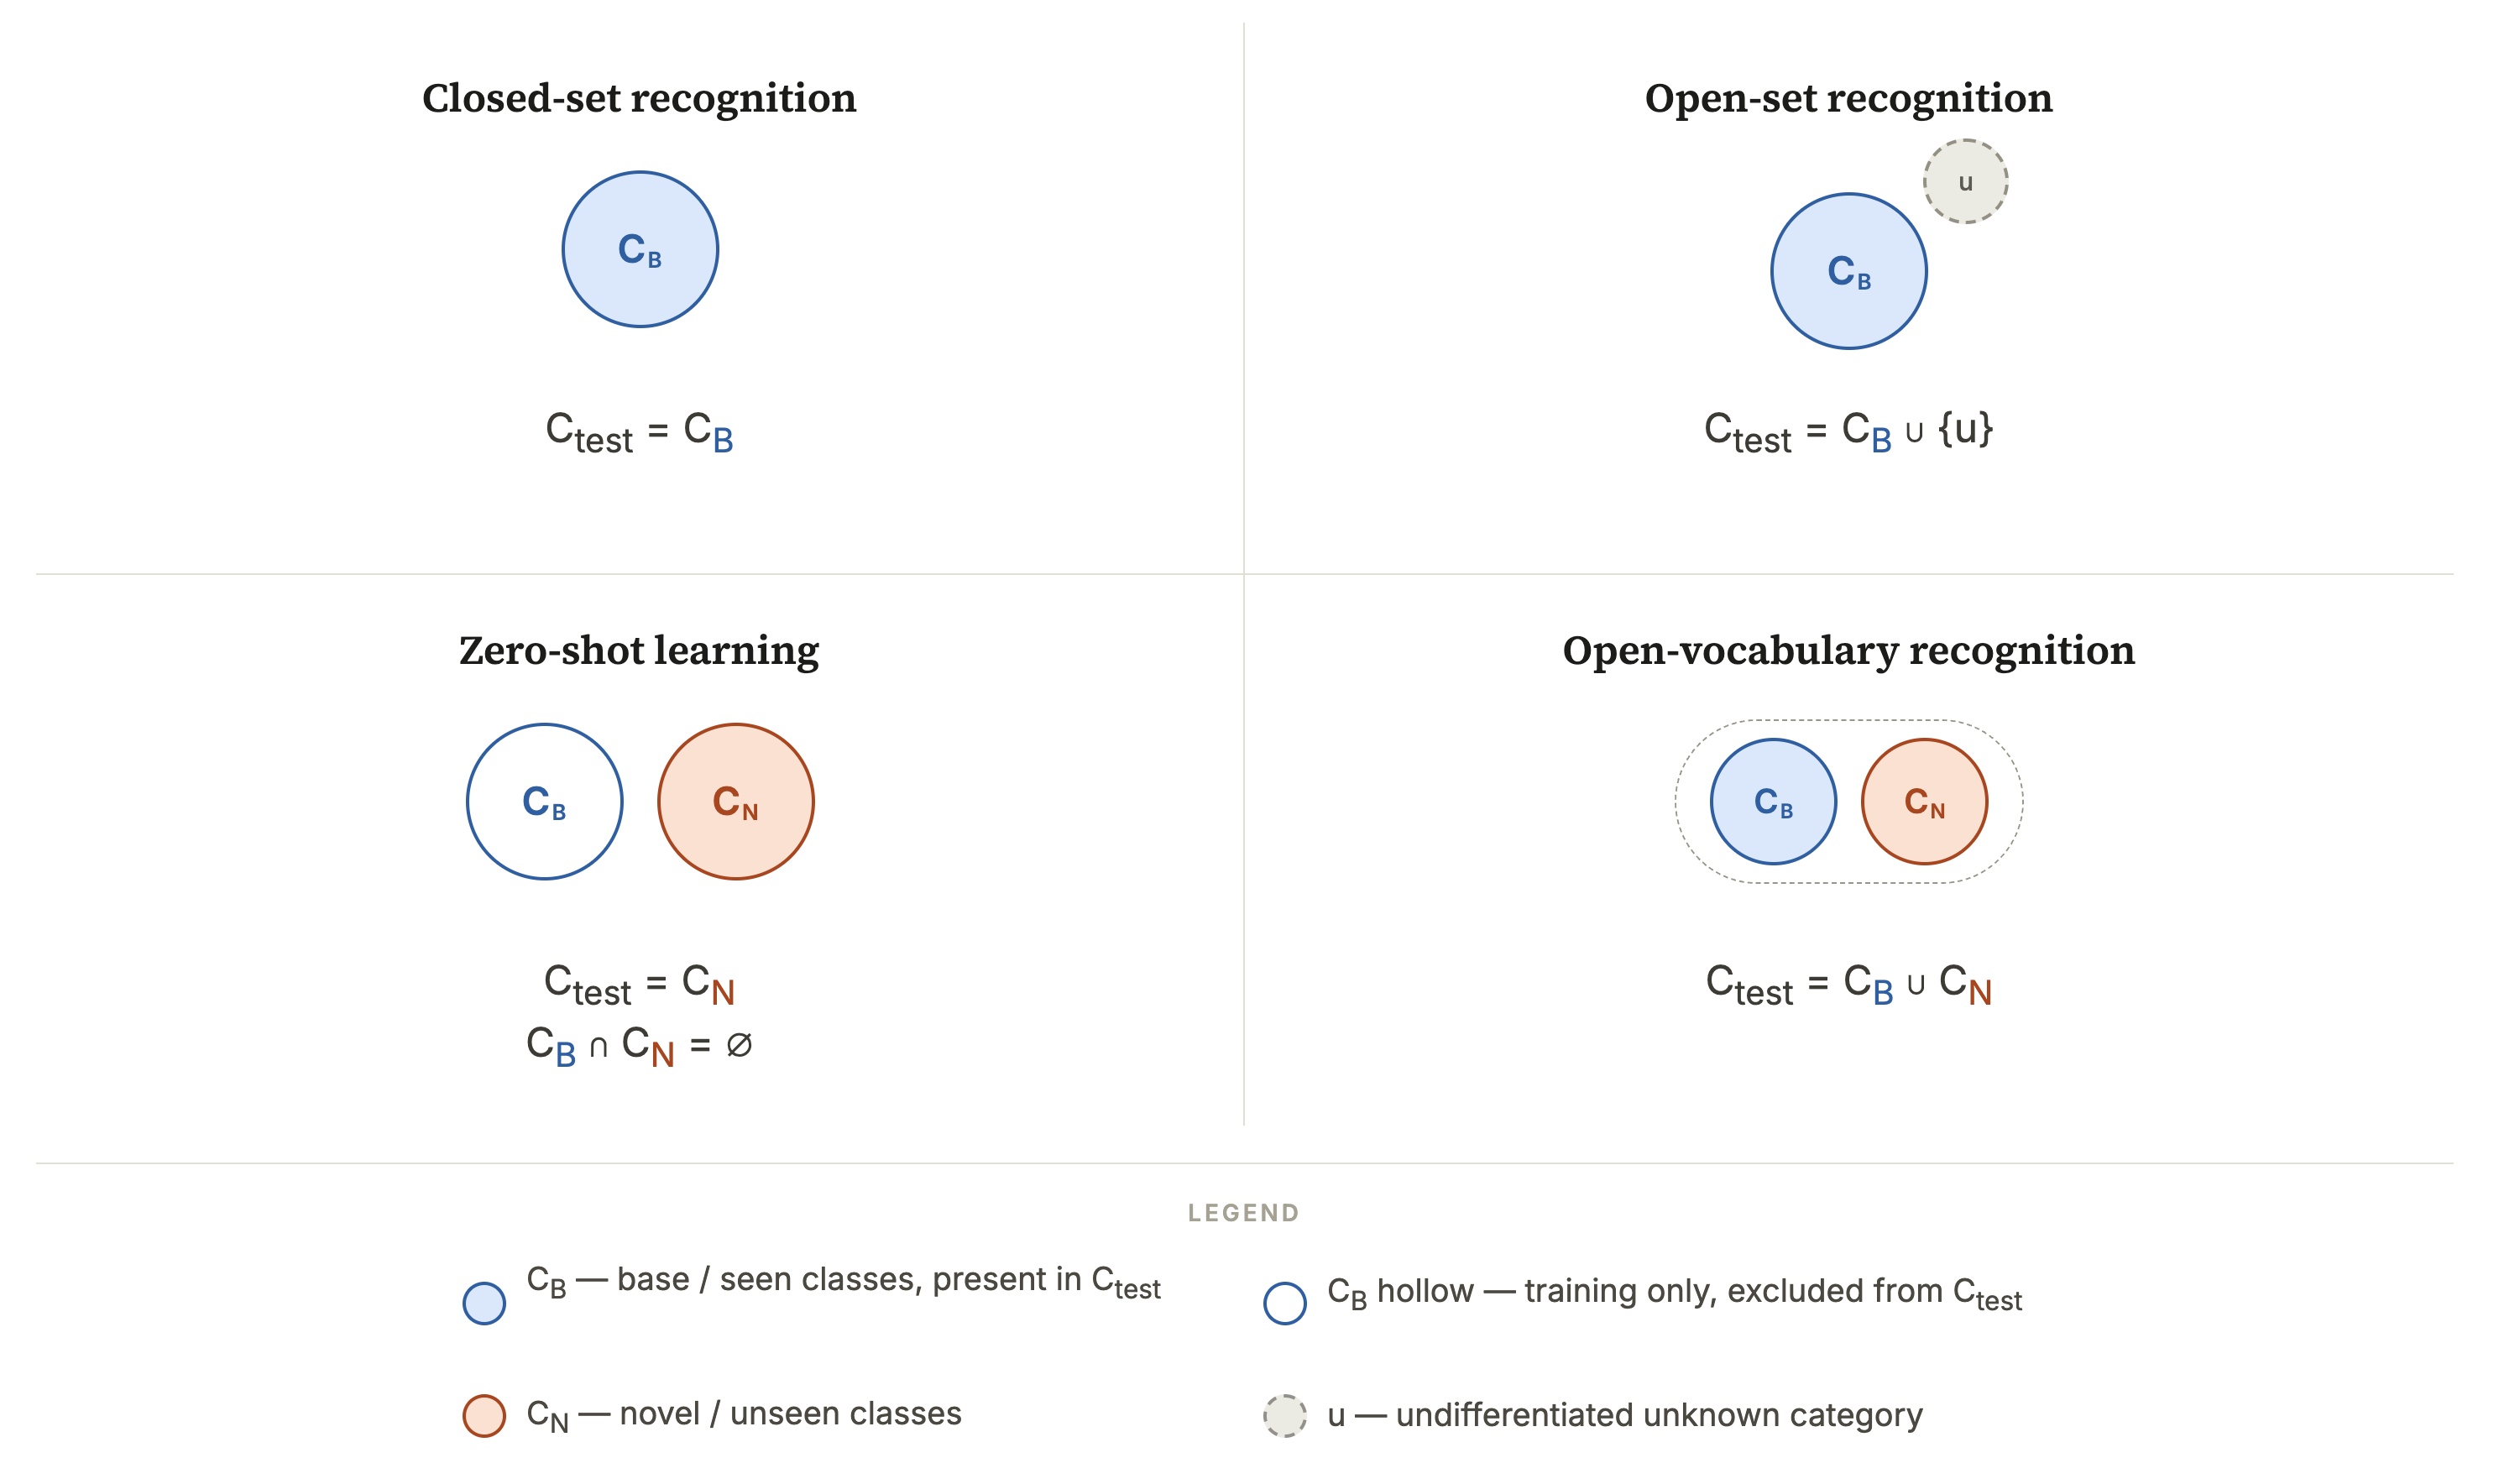
\includegraphics[width=\textwidth]{figures/cv_learning_paradigms_diagram.png}
  \caption{Label-space relationships for closed-set, open-set, zero-shot, and open-vocabulary recognition. \(C_B\), \(C_N\) and \(u\) denote base, novel, and unknown categories, respectively.}
  \label{fig:label-space-paradigms}
\end{figure}

\newpage
\noindent As summarised in Figure~\ref{fig:label-space-paradigms}, zero-shot and open-vocabulary learning are therefore related but distinct: zero-shot learning conventionally assumes a disjoint seen--unseen split and evaluates exclusively on \(C_N\), whereas open-vocabulary learning may draw on broader visual--language pretraining that is not constrained by this partition \cite{wu2024openvocabulary,zhu2024openvocabulary,cao2025zeroshot}. Modern open-vocabulary approaches commonly exploit image--text supervision or pretrained \glspl{VLM}, whose language-aligned representations provide semantic knowledge beyond the categories explicitly annotated in the task-specific training data \cite{wu2024openvocabulary,zhu2024openvocabulary}.

Large-scale pretraining has further enabled models to be transferred across downstream vision tasks and conditioned through prompts without conventional retraining \cite{reshadi2026deeplearningcv,Transformers4Vision}. \glspl{VLM} can use textual prompts to specify semantic concepts, while promptable segmentation models can use spatial prompts such as points or bounding boxes to specify regions of interest \cite{wu2024openvocabulary,BG38-segment-anything}. When such prompts are supplied only at inference time the pretrained model parameters remain unchanged, whereas fine-tuning instead updates model parameters using task-specific supervision \cite{BG38-segment-anything,reshadi2026deeplearningcv}.

\noindent Within detection, \emph{\gls{ZSD}} extends zero-shot learning by requiring both localisation and classification of objects belonging to categories that were not available as labelled classes during task-specific training \cite{cao2025zeroshot,zhu2024openvocabulary}. The broader experimental comparison in this dissertation is described as \emph{zero-shot localisation}, because the evaluated pretrained models may return bounding boxes, masks or other spatial predictions rather than conforming strictly to conventional \gls{ZSD} \cite{BG38-segment-anything,cao2025zeroshot}. A model is evaluated under this setting when it is applied to the \gls{MDWD} or \gls{MTSD} without labelled target-dataset training or task-specific parameter optimisation, while making no assumption that related concepts were absent from its original pretraining data \cite{wu2024openvocabulary,zhu2024openvocabulary,cao2025zeroshot}.

\subsection{Supervised Object Detection}
\label{sec:bg-supervised-od}
Supervised \gls{OD} learns to predict object categories and bounding boxes from annotated imagery, combining semantic classification with spatial localisation \cite{zou2023objectdetection}. In the conventional closed-set setting introduced in Subsection~\ref{sec:bg-cv-paradigms}, the detector is trained for a predefined set of labelled categories. This formulation requires substantial manually annotated training data, and performance can deteriorate when the deployment distribution differs from that represented during training \cite{zou2023objectdetection}. This dependence is particularly relevant to specialised domains: \citeauthor{robinson2026rfdetrneuralarchitecturesearch} report that detectors heavily optimised for \gls{COCO} can generalise poorly to real-world datasets with substantially different distributions, including differences in the number of objects per image, number of classes and dataset size \cite{robinson2026rfdetrneuralarchitecturesearch}.

\newpage
\noindent The development of \gls{DL}-based \gls{OD} has been shaped by a recurring trade-off between localisation accuracy, computational efficiency and deployment complexity \cite{zou2023objectdetection}. Region-based detectors established the two-stage paradigm by separating candidate-region generation from classification and bounding-box refinement \cite{girshick2014rcnn,girshick2015fastrcnn,ren2015faster}. Single-stage detectors instead perform localisation and classification directly from image features, substantially reducing inference cost and enabling real-time operation \cite{redmon2016you,liu2016ssd}. Transformer-based detectors introduced a further formulation based on direct set prediction, learned object queries and bipartite matching, reducing reliance on hand-designed components such as anchor boxes and \gls{NMS} \cite{carion2020end}. These families are reviewed below, followed by their application to waste and traffic-sign monitoring and the rationale for the detectors evaluated in this dissertation.

\subsubsection{Problem Formulation and Recurring Design Considerations}
\label{sec:bg-od-formulation}
Given an input image, a detector produces a set of predictions, each comprising a bounding box, a class label and a confidence score \cite{zou2023objectdetection}. During evaluation, predictions are matched to annotated \gls{GT} instances according to spatial overlap, commonly measured using \gls{IoU}, from which precision--recall curves and average-precision measures are derived \cite{lin2014coco}. Although this formulation is shared across detector families, architectures differ considerably in how candidate objects are represented, assigned during training and filtered during inference.

Central to this variation is label assignment, the process by which \gls{GT} objects are associated with candidate predictions during optimisation. Dense detectors generate predictions at many spatial locations and feature-map scales, requiring rules that determine which locations constitute positive training examples for each object \cite{zou2023objectdetection,tian2019fcos}. Earlier architectures relied on predefined anchor boxes of differing scales and aspect ratios, whereas anchor-free approaches predict object geometry directly from feature-map locations, removing anchor-specific hyperparameters that may be poorly matched to a new dataset \cite{tian2019fcos}. The assignment strategy is consequential because insufficient positive assignments impair localisation, particularly for small objects whose extent covers very few candidate locations.

Dense assignment strategies produce a high volume of predictions, giving rise to duplicate detections. Detection heads of this kind commonly produce several overlapping boxes for the same object and therefore employ \gls{NMS}, which ranks predictions by confidence and suppresses lower-confidence boxes whose overlap with a retained detection exceeds a threshold \cite{zou2023objectdetection}. Although effective, \gls{NMS} is a heuristic stage outside the learned model and may suppress legitimate neighbouring objects where instances occur in close proximity. End-to-end set-prediction detectors instead learn to produce one prediction per object directly, avoiding conventional duplicate suppression \cite{carion2020end, wang2024yolov10}.

\noindent These assignment and suppression mechanisms are further complicated by object scale, a persistent challenge in its own right. Street imagery contains objects ranging from large foreground instances to targets occupying only a few pixels. \Glspl{FPN} address this by combining semantically strong, low-resolution features with spatially precise, higher-resolution representations through top-down and lateral connections, allowing predictions at several resolutions rather than exclusively from the most heavily downsampled feature map \cite{lin2017fpn}. Small-object performance nevertheless remains substantially weaker than that for medium and large objects across many architectures, motivating the size-stratified reporting of average precision adopted by \gls{COCO} \cite{lin2014coco,zou2023objectdetection}.

\subsubsection{Two-Stage Region-Based Detectors}
\label{sec:bg-od-two-stage}
The \gls{R-CNN} family established the two-stage paradigm and dominated early \gls{DL}-based detection. \gls{R-CNN} itself generated class-agnostic candidate regions through selective search and processed each independently through a convolutional network before classification and box refinement, demonstrating the value of learned representations for localisation but at substantial computational redundancy \cite{girshick2014rcnn}. This redundancy was subsequently resolved by Fast \gls{R-CNN}, which computed convolutional features once per image and projected each proposal onto the shared feature map through \gls{RoI} pooling, enabling joint training of classification and regression \cite{girshick2015fastrcnn}. The remaining bottleneck of external region proposal was then eliminated by Faster \gls{R-CNN}, which integrated proposal generation directly into the network through a trainable \gls{RPN} sharing features with the detection head, establishing the characteristic two-stage structure of proposal followed by proposal-specific classification and refinement \cite{ren2015faster}. This progressive refinement gave two-stage systems strong localisation accuracy, further strengthened by integration with the \gls{FPN}, which fuses low-resolution semantic features with higher-resolution spatial detail across scales \cite{lin2017fpn,zou2023objectdetection}. The staged structure nevertheless introduces additional computation relative to direct prediction, a limitation that became increasingly consequential as detection expanded into video, autonomous systems and embedded applications where latency and throughput matter as much as benchmark accuracy \cite{redmon2016you,zou2023objectdetection}.

\subsubsection{Single-Stage Detectors}
\label{sec:bg-od-single-stage}
Single-stage detectors instead remove the explicit proposal-and-refinement separation and predict locations and categories directly from image features \cite{redmon2016you,liu2016ssd}. The original \gls{YOLO} treated detection as a unified regression problem, dividing the image into a grid and predicting boxes, objectness and class probabilities in a single network evaluation, yielding a substantial speed improvement at the cost of greater localisation error and weaker small-object performance \cite{redmon2016you}. \gls{SSD} adopted a comparable single-stage formulation but predicted from feature maps at several resolutions instead, so that smaller objects were represented by higher-resolution features and larger objects by deeper features with broader receptive fields \cite{liu2016ssd}. This multi-resolution design foreshadowed the multi-scale principle that became standard throughout later single-stage detectors.

Predicting densely across the entire image in this way, however, introduces an extreme imbalance between foreground objects and background candidate locations. RetinaNet identified this imbalance as a principal contributor to the historical accuracy gap between one- and two-stage detectors and introduced Focal Loss to down-weight easily classified examples, demonstrating that the gap arose partly from how dense predictions were supervised rather than from the single-stage formulation itself \cite{lin2017focal}. Combined with stronger backbones and improved assignment strategies, these developments progressively narrowed the separation between single- and two-stage performance \cite{zou2023objectdetection}. Single-stage architectures have consequently become prominent in deployment-oriented \gls{OD}, particularly where large image volumes must be processed under latency or hardware constraints. This balance is pertinent to municipal monitoring, where imagery may be acquired repeatedly from mobile or fixed platforms and where computational cost governs the practicality of large-scale deployment.

\subsubsection{The \gls{YOLO} Family}
\label{sec:bg-yolo}
The \gls{YOLO} family represents the principal lineage of single-stage real-time detection, and several generations illustrate the architectural changes that have progressively transformed it. \gls{YOLO}2 introduced anchor-based prediction, batch normalisation and multi-scale training, exposing an explicit speed--accuracy trade-off through variable input resolution \cite{redmon2017yolo9000}. \gls{YOLO}3 extended prediction across multiple feature scales using a deeper residual backbone \cite{redmon2018yolov3}. \gls{YOLO}4 combined cross-stage partial connections, path aggregation and extensive augmentation to improve accuracy while preserving real-time inference \cite{bochkovskiy2020yolov4}. \gls{YOLO}7 introduced Extended Efficient Layer Aggregation Networks and training-time refinements that add no inference cost \cite{wang2023yolov7}, while \gls{YOLO}9 proposed Programmable Gradient Information to mitigate information loss in deep detector architectures \cite{wang2024yolov9}.

A more substantial change appeared with \gls{YOLO}10, which introduced consistent dual label assignment, whereby a one-to-many head provides rich supervision during training while a one-to-one head supports non-redundant predictions so that inference no longer requires \gls{NMS} \cite{wang2024yolov10}. This development substantially narrowed the distinction that had previously separated dense \gls{YOLO}-style detectors from the set-prediction formulation used by Transformer-based detectors such as \gls{DETR}.

\newpage
\noindent The recent generations leading to the models evaluated in this dissertation illustrate materially different architectural emphases. \gls{YOLO}11 retains a predominantly convolutional backbone--neck--head structure while introducing compact C3k2 blocks and the C2PSA attention module to strengthen spatial feature modelling, with an anchor-free head available across several capacity scales \cite{yolo11}. \gls{YOLO}12 moves the lineage towards attention-centric feature modelling through Area Attention, which partitions attention computation to retain a broad receptive field at reduced cost, and Residual Efficient Layer Aggregation Networks for stable optimisation \cite{tian2025yolov12}. It integrates attention more centrally into the representation without becoming a conventional \gls{VIT}, preserving the real-time latency characteristic of \gls{YOLO} detectors while adopting the attention-based feature modelling associated with Transformer architectures.

\gls{YOLO}26 shifts emphasis towards native end-to-end and edge-oriented inference, whereby a dual-head design yields \gls{NMS}-free one-to-one predictions, with the one-to-many head used only during training, while Distribution Focal Loss is removed to simplify the inference graph \cite{jocher2026yolo26}. Its training procedure is adapted accordingly, with Small-Target-Aware Label Assignment improving positive-sample coverage for objects spanning few candidate locations, Progressive Loss stabilising optimisation as reliance shifts towards the one-to-one head, and the \gls{MuSGD} optimiser supporting convergence under this dual-head regime \cite{jocher2026yolo26}. These developments are directly pertinent to small targets and constrained hardware, although architectural simplification does not guarantee superior accuracy or latency on every dataset.

\subsubsection{Transformer-Based Detection}
\label{sec:bg-transformer-detection}
\gls{DETR} introduced a distinct formulation of \gls{OD} based on direct set prediction, departing entirely from the region-proposal and dense-anchor mechanisms underlying earlier detectors \cite{carion2020end}. An image representation extracted by a convolutional backbone is passed through a Transformer encoder, which models relationships across the feature map and, in doing so, makes contextual information from spatially distant regions available during subsequent query refinement. A decoder then attends over a fixed set of learned object queries, each of which is refined into a class prediction and bounding box, with one-to-one bipartite matching during training encouraging every \gls{GT} instance to be represented by exactly one prediction and thereby removing the need for anchors and \gls{NMS} \cite{carion2020end,yu2025detrreview}.

The original \gls{DETR} nevertheless converged slowly, imposed considerable computational cost through global self-attention on high-resolution features, and performed comparatively weakly on small objects \cite{carion2020end,yu2025detrreview}. Deformable \gls{DETR} addressed these limitations by sampling a small set of learned locations around reference points across several feature resolutions rather than attending densely over every position, a multi-scale deformable attention mechanism that reduced cost, accelerated convergence and gave higher-resolution features direct influence on query refinement \cite{zhu2021deformabledetr}.

\gls{RT-DETR} subsequently adapted this Transformer-based formulation to real-time constraints through a hybrid encoder that separates intra-scale interaction from cross-scale fusion, avoiding indiscriminate Transformer processing across all feature levels, together with uncertainty-minimal query selection that initialises object queries from high-quality encoder features \cite{zhao2024rtdetr}. The resulting detector demonstrated that an end-to-end, \gls{NMS}-free Transformer could compete directly with real-time \gls{YOLO} models in both accuracy and latency \cite{zhao2024rtdetr}. The contrast between contemporary convolutional and Transformer-based detectors is therefore more nuanced than the historical division between fast single-stage and accurate but expensive alternatives. Both now incorporate multi-scale representation, sophisticated assignment and end-to-end prediction, and their remaining differences concern how spatial context is modelled, how candidate objects are represented, the computational profile of extractor and decoder, and their behaviour under dataset-specific conditions such as small targets, clutter and densely positioned instances \cite{yu2025detrreview}.

\glsreset{RF-DETR}
\subsubsection{The \gls{RF-DETR} Model}
\label{sec:bg-rfdetr}
\gls{RF-DETR} is a recent real-time end-to-end detector that develops the \gls{DETR} lineage by combining query-based detection with large-scale self-supervised pretraining and architecture optimisation \cite{robinson2026rfdetrneuralarchitecturesearch}. Building upon \gls{LW-DETR}, it replaces the backbone with a pretrained \gls{DINO}v2 \gls{VIT}, so that detection begins from representations learnt through large-scale self-supervision rather than solely from the target dataset, while retaining multi-scale features supplied to a query-based decoder, one-to-one matching during training and \gls{NMS}-free inference \cite{robinson2026rfdetrneuralarchitecturesearch}. This design is motivated by \citeauthor{robinson2026rfdetrneuralarchitecturesearch}'s observation that architectures and training procedures heavily optimised for \gls{COCO} do not necessarily retain their performance on datasets with different numbers of objects, categories and examples \cite{robinson2026rfdetrneuralarchitecturesearch}.

Beyond its backbone and query-based decoding, \gls{RF-DETR} additionally employs \gls{NAS}, which automates the discovery of architectural configurations by searching over structural choices rather than fixing them by hand. Its weight-sharing variant allows candidate configurations to share a single set of trained weights during the search, substantially reducing the cost of exploring the accuracy--latency trade-off \cite{robinson2026rfdetrneuralarchitecturesearch}. The search varies input resolution, patch size, decoder depth, query count and the number of windows per attention block within this shared framework, yielding a family of configurations that occupy different operating points rather than uniformly scaled replicas. Consequently, the nominal size labels assigned to \gls{RF-DETR} variants do not correspond to equally named \gls{YOLO} models in parameter count, resolution or capacity, a distinction considered explicitly in the model-scale comparisons of Subsection~\ref{sec:supervised-model-ablation}.

\subsubsection{Supervised Detection in Municipal Monitoring}
\label{sec:bg-od-municipal}
Municipal monitoring places supervised \gls{OD} in substantially less controlled conditions than many conventional recognition tasks. Waste may vary considerably in shape, material and appearance and often occurs in cluttered or overlapping arrangements, whereas traffic signs are visually more structured but frequently occupy only a small proportion of the image and are affected by distance, occlusion and illumination \cite{BG17-small-signs,BG20-sign-glare}. These differences make detector selection dependent not only on predictive accuracy, but also on how well an architecture handles the visual characteristics and computational requirements of the target domain.

The \gls{YOLO} family has consequently been prominent in applied municipal-monitoring research, particularly where repeated image processing favours low-latency inference. In waste monitoring, \citeauthor{decarolis2020yolotrashnet} developed YOLO TrashNet from \gls{YOLO}3 for the detection and reporting of abandoned waste \cite{decarolis2020yolotrashnet}, demonstrating an early use of \gls{OD} within an operational reporting workflow. More recently, \gls{YOLO}8, \gls{YOLO}9 and \gls{YOLO}10 were compared on pLitterStreet before the selected detector was applied to Google Street View imagery for spatial litter mapping \cite{espinosa2025litter}, and \gls{YOLO}11 was used to detect both garbage and potholes within a municipal reporting workflow \cite{reddy2025yologarbagepothole}. These studies illustrate a shift from recognising waste in isolation towards using detections as spatial observations of street-level conditions.

A similar emphasis on efficient detection is evident in traffic-sign research, although the small image-space extent of signs has encouraged greater attention to feature preservation and multi-scale representation. A series of modifications to \gls{YOLO}5 and \gls{YOLO}7 introduced coordinate, channel and spatial attention, dynamic label assignment and multi-scale feature fusion specifically to improve small-sign detection under complex road conditions \cite{wang2023improvedtrafficsign,shi2023scyolo,mahadshetti2024signyolo}, while \citeauthor{liu2024yolots} developed YOLO-TS from \gls{YOLO}8n to reduce computational demand while retaining performance on small traffic signs \cite{liu2024yolots}. Across this work, small-target representation, feature fusion, attention and deployment cost are treated as interdependent design considerations rather than accuracy in isolation.

Transformer-based detectors provide a contrasting approach through query-based set prediction and attention-based feature modelling. Recent traffic-sign studies suggest that these architectures can also operate within real-time constraints when adapted to the domain. \citeauthor{lin2025tsdetr} proposed TS-DETR, combining positive- and negative-sample augmentation with multi-scale feature integration to address small targets and class imbalance \cite{lin2025tsdetr}, while \citeauthor{dong2026hasdetr} adapted \gls{RT-DETR} through HAS-DETR, introducing high-frequency feature preservation, cross-scale fusion and a dedicated small-target enhancement head \cite{dong2026hasdetr}. Both studies retain the end-to-end Transformer formulation while explicitly modifying it around the characteristics of traffic-sign imagery. Early infrastructure studies have also begun to evaluate \gls{RF-DETR} directly against \gls{YOLO} for road-surface and road-damage assessment \cite{kurrey2026roadsurface,amores2026roaddamage}, although its application base remains considerably smaller than that of either \gls{YOLO} or \gls{RT-DETR}.

More direct comparisons indicate that neither detector family is uniformly preferable. \citeauthor{kumar2026gvp} compared \gls{YOLO}8, \gls{YOLO}10, \gls{YOLO}11m and \gls{RT-DETR} for monitoring garbage-vulnerable points using a street-side camera and \gls{IoT} infrastructure \cite{kumar2026gvp}. The system coupled detection with temporal analysis of dumping and cleaning activity, placing the comparison within an operational waste-monitoring setting rather than an isolated benchmark. In traffic-sign condition assessment, \gls{YOLO}11 and \gls{RT-DETR} were compared for detecting fading and delamination from vehicle-acquired roadway imagery \cite{pandey2026signcondition}. Relative performance depended on the defect: \gls{YOLO}11 performed better for fading and achieved lower end-to-end runtime, whereas \gls{RT-DETR} showed a smaller advantage for delamination. This suggests that architectural preference can vary even within the same municipal asset class.

\subsubsection{Selection of Detection Architectures}
\label{sec:bg-selection-od}
Taken together, the literature indicates that detector performance is strongly dependent on the visual and operational characteristics of the target domain. Waste monitoring involves irregular object geometry, heterogeneous appearance, clutter and frequent co-occurrence, whereas traffic-sign monitoring places greater emphasis on small-object localisation, viewing distance, illumination and, where condition is considered, subtle degradation cues. Performance reported on generic benchmarks, or within one municipal domain, therefore cannot be assumed to transfer directly to another \cite{robinson2026rfdetrneuralarchitecturesearch,pandey2026signcondition}.

The detectors evaluated in this dissertation were selected to examine these differences across two contemporary real-time detection lineages. \gls{YOLO}11, \gls{YOLO}12 and \gls{YOLO}26 represent recent stages in the development of the single-stage family, spanning predominantly convolutional feature modelling, more attention-centric representations and native end-to-end prediction \cite{yolo11,tian2025yolov12,jocher2026yolo26}. \gls{RF-DETR} provides a Transformer-based counterpart operating within the same real-time setting, but differs through query-based prediction, a self-supervised pretrained backbone and architecture-search-based scaling \cite{robinson2026rfdetrneuralarchitecturesearch}. Rather than assuming that either lineage will transfer uniformly across domains, all detectors are evaluated under a common protocol on both datasets, as described in Section~\ref{sec:supervised-detection-methodology}.

\subsection{Zero-Shot and Prompt-Based Object Localisation}
\label{sec:bg-zero-shot}
The development of large-scale pretrained visual models has broadened the means by which localisation tasks can be specified beyond the fixed category spaces associated with conventional supervised \gls{OD}. Rather than learning every target category exclusively from task-specific bounding-box annotations, contemporary approaches increasingly exploit visual representations acquired from large and heterogeneous datasets, with the target concept supplied through language, visual exemplars or spatial prompts at inference time \cite{bommasani2021opportunities,radford2021learning,xiao2024florence2}. This progression has produced several related but architecturally distinct approaches, including open-vocabulary detection, promptable segmentation and grounded \glspl{VLM}. Their principal attraction lies in the ability to transfer pretrained capabilities to new concepts with little or no target-domain supervision, although this flexibility remains dependent on the correspondence between the target domain, the pretraining distribution and the prompts used to specify the task.

\subsubsection{Foundation Models and Zero-Shot Visual Transfer}
\label{sec:bg-foundation-models}
The concept of a \gls{FM} describes a model pretrained at scale on broad data and subsequently transferable across a range of downstream tasks rather than optimised exclusively for a single predefined objective \cite{bommasani2021opportunities}. In \gls{CV}, an important development towards this formulation was the use of natural-language supervision to replace or complement manually defined class vocabularies. Radford et al.~\cite{radford2021learning}, for example, trained \gls{CLIP} contrastively on 400 million image--text pairs, learning a shared representation in which visual concepts could subsequently be referenced through natural language. This enabled zero-shot transfer across a diverse collection of recognition tasks without dataset-specific parameter optimisation and established image--language pretraining as a practical mechanism for transferring visual knowledge beyond a fixed training taxonomy.

Large-scale pretraining does not, however, remove the distinction between zero-shot, few-shot and supervised adaptation. As defined in Subsection~\ref{sec:bg-cv-paradigms}, zero-shot inference applies the pretrained capability without updating model parameters on the target dataset, whereas few-shot methods introduce a limited amount of target-specific evidence through examples or restricted adaptation. Fully supervised approaches make substantially greater use of labelled target data and consequently offer greater opportunity for specialisation. The trade-off is therefore between adaptability and target-domain optimisation: zero-shot systems reduce annotation and retraining requirements but remain constrained by what their pretrained representations encode, while supervised models can learn distinctions that are specific to a local taxonomy or visual environment.

The experiments reported by Radford et al.~\cite{radford2021learning} illustrate that this relationship is not simply monotonic with the number of labelled examples. Their zero-shot formulation was competitive with low-shot linear probing in several settings, while the authors also observed that language alone remains inadequate for visual concepts that are difficult to express textually and that supervised performance remained stronger on many datasets. Zero-shot capability should therefore be understood as a transfer property rather than an assumption of equivalent performance to task-specific supervision.

Subsequent \glspl{FM} have extended this principle beyond image-level recognition towards multiple spatial and semantic tasks. Florence-2, for example, adopts a unified sequence-to-sequence architecture in which textual task prompts can elicit captioning, detection, grounding or segmentation outputs from the same model \cite{xiao2024florence2}. Its pretraining corpus contains 5.4 billion annotations across 126 million images spanning image-, region- and pixel-level supervision. This progression is important because it shifts the role of prompting from selecting among image-level semantic categories towards specifying both the visual concept and the form of spatial information required from the model.

\subsubsection{Promptable Segmentation and the Segment Anything Family}
\label{sec:bg-sam}

A parallel development occurred in segmentation through the introduction of promptable visual segmentation. The original \gls{SAM} separated image encoding from prompt-conditioned mask prediction, allowing a target region to be specified using spatial cues such as points or bounding boxes rather than through a fixed semantic category \cite{kirillov2023segment}. \gls{SAM}~2 extended this formulation from static images to video through a memory-based architecture capable of propagating and refining prompted objects across frames while retaining the point-, box- and mask-based interaction of the original model \cite{ravi2024sam2}. The principal capability of these models was therefore spatial generalisation: they could delineate previously unseen objects when supplied with an indication of which object should be segmented, but the prompt itself did not necessarily communicate semantic identity.

This distinction motivated combinations of promptable segmentation with language-grounded detection. Grounded SAM, for example, couples Grounding DINO with \gls{SAM}, using a textual query to identify corresponding regions before supplying the resulting boxes to the segmentation model \cite{ren2024grounded}. The resulting pipeline combines semantic flexibility with pixel-level localisation without requiring the segmentation component itself to perform open-vocabulary recognition.

\gls{SAM}~3 subsequently integrates semantic concept prompting more directly into the Segment Anything formulation. Rather than requiring the location of an individual instance to be provided in advance, the model introduces promptable concept segmentation, in which short noun phrases, image exemplars or combinations of the two can be used to detect and segment all matching instances within an image or video \cite{meta2025sam3}. Positive and negative exemplars can additionally refine the intended concept, providing a form of visual few-shot specification alongside language prompting. This broader capability also introduces semantic ambiguity absent from purely spatial prompting, since noun phrases may admit multiple visual interpretations and their correspondence can be affected by occlusion, blur or subjective descriptors. Prompt formulation and exemplar selection therefore become part of the effective task definition rather than merely an interface choice.

\subsubsection{Open-Vocabulary and Language-Grounded Localisation}
\label{sec:bg-open-vocabulary}

The development of open-vocabulary localisation similarly reflects the movement from image-level language alignment towards region-level grounding. While models such as \gls{CLIP} demonstrated that visual representations could be associated with arbitrary textual concepts, image-level contrastive supervision does not itself establish where those concepts occur within an image \cite{radford2021learning}. Open-vocabulary detection addresses this limitation by explicitly aligning textual representations with spatial image regions, allowing language to specify the objects to be localised.

Grounding DINO represents a prominent development of this formulation by integrating grounded language supervision with a Transformer-based detector \cite{liu2024grounding}. Rather than attaching language only to the final classification stage, the architecture introduces cross-modal interaction during feature enhancement, query selection and decoding, enabling categories and referring expressions to influence the localisation process throughout the network. The model can consequently detect objects specified through category names or descriptive expressions without requiring the corresponding target dataset to have been used for task-specific training.

This flexibility differentiates grounded localisation from conventional closed-set \gls{OD}, where adding a new semantic category generally requires additional labelled examples and model adaptation. It also differs from the earlier Segment Anything formulation, in which the prompt primarily identifies \emph{where} the target object lies rather than \emph{what} concept should be found. Language-grounded localisation must infer both simultaneously, increasing semantic flexibility but also introducing sensitivity to terminology. This is particularly relevant to specialised monitoring taxonomies, where an operational category may be visually meaningful within a local context while differing from the language and concepts represented during large-scale pretraining.

\subsubsection{Locate Anything}
\label{sec:bg-locate-anything}

The extension of language grounding into generative \glspl{VLM} has introduced a further localisation formulation in which spatial coordinates are represented within the model's output sequence. Conventional generative grounding commonly serialises a bounding box into several coordinate tokens that are decoded sequentially, allowing spatial prediction to share the same general interface as textual generation but imposing both computational and structural limitations when numerous objects must be returned \cite{nvidia2026locateanything}.

LocateAnything addresses this limitation through Parallel Box Decoding, treating geometric entities such as bounding boxes and points as coupled spatial units rather than independent tokens \cite{nvidia2026locateanything}. Its large-scale grounding framework is trained on more than 138 million localisation samples and supports multiple forms of visual grounding and detection within a common vision--language architecture. By decoding the coordinates belonging to a geometric unit in parallel, the model seeks to preserve their spatial relationship while reducing the sequential inference cost associated with autoregressive coordinate generation.

This formulation is particularly relevant to comparisons with conventional \gls{OD} because it produces explicit spatial predictions while retaining the semantic flexibility of a generative \gls{VLM}. The distinction nevertheless remains important: localisation is generated through a vision--language decoding process rather than a conventional detector head, so its output structure, confidence information and inference behaviour need not correspond directly to those of supervised detectors. The LocateAnything study additionally considers dense and overlapping scenes, where maintaining separation between adjacent predictions is especially demanding, making the approach relevant to localisation problems containing multiple closely positioned instances.

\subsubsection{Vision--Language Models and Grounded Visual Reasoning}
\label{sec:bg-vlm-grounding}

Grounded \glspl{VLM} generalise this formulation further by combining visual localisation with the broader language-generation capabilities of multimodal models. Whereas a dedicated detector is principally optimised to produce categories, locations and confidence scores, a \gls{VLM} can place spatial predictions within a richer generated response that also describes objects, relationships or contextual properties. Florence-2 demonstrates an intermediate form of this unification, using textual task prompts and a shared sequence representation for detection, grounding, segmentation and language-based visual understanding \cite{xiao2024florence2}, while more recent generative grounding models incorporate coordinates directly into multimodal output sequences \cite{nvidia2026locateanything}.

The broader output space provides greater flexibility but creates additional reliability requirements. Spatial predictions must remain geometrically valid and complete while the generated semantic interpretation must remain grounded in the visual evidence. Recent evaluation of multimodal language models has shown that linguistically plausible outputs do not necessarily imply faithful visual grounding, with errors arising from target-region binding, transcription and language-prior effects even where the visual evidence is comparatively clear \cite{wang2026symbolconsistency}. Such behaviour is particularly relevant to roadside imagery containing text, symbols or multiple similar objects, since a plausible semantic response may still refer to the wrong visual instance.

Grounded \glspl{VLM} should therefore be distinguished from specialised localisation architectures despite their ability to emit bounding boxes or points. Their advantage lies in combining localisation with semantic and contextual interpretation, while their broader generative formulation introduces additional opportunities for omission, spatial inconsistency and visually unsupported output. Whether this additional flexibility provides practical value consequently depends on the extent to which the monitoring task requires reasoning beyond object presence and location.

\subsubsection{World Foundation Models and the NVIDIA Cosmos Family}
\label{sec:bg-cosmos}

\Glspl{WFM} broaden the scope of foundation modelling from static visual recognition towards representations of physical environments and their evolution over time. NVIDIA's Cosmos platform defines a \gls{WFM} as a broadly pretrained world model that can subsequently be specialised for downstream physical-\gls{AI} applications, using large-scale video data to acquire general representations of visual dynamics before post-training for particular environments or tasks \cite{nvidia2025cosmosplatform}. This differs from conventional \gls{OD} and visual grounding because the intended representation encompasses not only object identity and location but also temporal behaviour and physical interaction.

Cosmos-Reason1 develops the reasoning component of this formulation through multimodal models trained to interpret video using representations of physical common sense and embodied reasoning \cite{nvidia2025cosmosreason1}. Its emphasis lies on spatial, temporal and physical relationships and on producing reasoned natural-language responses or embodied decisions, rather than on replacing a dedicated object detector. The Cosmos Reason2 models evaluated in this dissertation are reasoning \glspl{VLM} from this family, applied here to static images and bounding-box generation rather than video prediction or action generation \cite{nvidia2025cosmosreason2}. Cosmos~3 subsequently extends the family towards an omnimodal architecture capable of jointly processing and generating language, images, video, audio and action sequences, thereby integrating visual understanding, generation and action modelling within a common framework \cite{nvidia2026cosmos3}.

For municipal visual monitoring, the relevance of this broader modelling direction lies in the distinction between recognising an object and interpreting its context. A dedicated detector may establish that waste or a traffic sign is present, whereas a physically grounded model may potentially reason about temporal persistence, spatial relationships or the surrounding scene. The literature supporting these models is, however, presently concentrated primarily on general visual grounding, robotics, autonomous systems and embodied \gls{AI}, rather than on municipal inspection itself. Their applicability to street-level waste and infrastructure monitoring therefore remains an empirical question rather than an established result.

Taken together, the literature reflects a progression from representations learned for fixed visual categories towards increasingly general systems in which the required concept, location or task can be communicated at inference time. Image--language pretraining first provided the semantic basis for zero-shot transfer, open-vocabulary detectors extended this alignment to spatial regions, promptable segmentation introduced flexible object delineation, and grounded \glspl{VLM} increasingly combine localisation with generated semantic or contextual interpretation. These approaches reduce dependence on task-specific annotation and make the queried vocabulary substantially more adaptable, but they do not eliminate the effects of domain shift, semantic ambiguity or prompt sensitivity. Their evaluation alongside supervised \gls{OD} on the \gls{MDWD} and \gls{MTSD} therefore provides a means of examining whether this increased flexibility can be realised without unacceptable losses in localisation reliability under municipal street-level conditions.



\subsection{Visual Representation Learning for Attribute Classification}
\label{sec:bg-representation}

    \subsubsection{Transfer Learning and Visual Representation Learning}
    \label{sec:bg-transfer-learning}

    \subsubsection{Self-Supervised Visual Representation Learning}
    \label{sec:bg-self-supervised}

    \subsubsection{DINOv3}
    \label{sec:bg-dinov3}

    \subsubsection{V-JEPA 2.1}
    \label{sec:bg-vjepa}

    \subsubsection{Supervised and Vision--Language Representations}
    \label{sec:bg-representation-baselines}

    \subsubsection{Adapting Pretrained Representations}
    \label{sec:bg-transfer-strategies}

    \subsubsection{Multi-Attribute Classification}
    \label{sec:bg-multiattribute}


\section{Deployment and Evaluation Considerations}
\label{sec:bg-deployment-evaluation}

\subsection{Deployment Architectures for Municipal Visual Monitoring}
\label{sec:bg-deployment}

    \subsubsection{Cloud, Edge and On-Device Computing}
    \label{sec:bg-edge}

    \subsubsection{Computational Efficiency and Deployment Constraints}
    \label{sec:bg-computational-efficiency}

\subsection{Evaluation Considerations for Visual Monitoring Systems}
\label{sec:bg-evaluation}

    \subsubsection{Robustness and Failure Analysis}
    \label{sec:bg-robustness}

    \subsubsection{Deployment-Oriented Evaluation}
    \label{sec:bg-deployment-evaluation-metrics}

\noindent\rule{\linewidth}{0.3pt}
\chapter{Methodology}
\label{ch:methodology}
This chapter sets out the empirical methodology used to address the research objectives of this dissertation. It first describes the construction, annotation, quality assurance, partitioning and preparation of the \gls{MDWD} and \gls{MTSD}, before detailing the three experimental tracks: supervised \gls{OD}, zero-shot prompt-based localisation, and traffic-sign attribute classification. For each track, the experimental configuration, model-specific procedures and evaluation protocol are defined to support a controlled and reproducible comparison of the investigated approaches.

\section{Overview of the Experimental Framework}
\label{sec:md-overview}
As established in Section~\ref{sec:research-approach}, the three experimental tracks are implemented within a common framework intended to preserve comparability where their objectives overlap, while retaining the methodological requirements specific to each task. The two localisation tracks operate on full street-level imagery from both datasets, whereas attribute classification uses \gls{GT} object crops from the \gls{MTSD}, allowing localisation performance to be assessed directly on complete scenes while separating traffic-sign characterisation from errors introduced by an upstream detector.

Within each dataset, supervised and zero-shot localisation are evaluated on the same fixed held-out test imagery, comprising 369 images for the \gls{MDWD} and 747 for the \gls{MTSD}, with predictions assessed against the same \gls{GT} annotations. Training-specific operations, including augmentation and parameter optimisation, are confined to the corresponding training partitions, while validation data are used where required for model selection, configuration and early stopping. Model-specific preprocessing is retained where necessary, rather than imposing transformations that would conflict with a given architecture's intended implementation.

For attribute classification, experimental partitions are instead inherited from the source imagery before object crops are generated, ensuring that all instances originating from the same image remain within a single partition. This preserves independence between the training, validation and test sets and provides a controlled basis for comparing the investigated visual representations and transfer strategies across the four annotated \gls{MTSD} attributes.

\newpage
\section{Dataset Construction and Preparation}
\label{sec:md-dataset-construction}
Two purpose-built Maltese street-level datasets were developed for the empirical work in this dissertation. Their taxonomies and operational rationale are established in Chapter~\ref{ch:bg-lit}, while this section describes their acquisition, annotation, \gls{QA}, partitioning and experimental preparation. To support reproducibility and future research, the \gls{MDWD} is publicly available through Roboflow\footnote{\url{https://universe.roboflow.com/um-dawl-ai-lab/mdwd-maltese-domestic-waste-dataset}} and, prior to the completion of this dissertation, a benchmark study introducing the dataset was accepted for publication at the 14th \gls{IEEE} European Conference on Visual Information Processing 2026.

\subsection{Image Acquisition and Source Corpus Formation}
\label{sec:md-acquisition}
Throughout this chapter, the retained imagery together with its verified annotations is referred to as the \emph{source corpus}, while task- and model-specific transformations subsequently applied to these data, including resizing, format conversion, augmentation and object cropping, produce the corresponding \emph{experiment-ready} representations. This distinction separates the characteristics of the original datasets from transformations introduced for individual experiments.

Both source corpora were collected by a third-party team using consumer-grade mobile devices, primarily while travelling on foot and, to a lesser extent, from moving vehicles, in which case imagery was captured by a passenger. Acquisition was opportunistic rather than route-constrained, covering northern, central and southern Malta together with Gozo without predefined spatial quotas. The resulting corpora therefore reflect conditions encountered during collection rather than a spatially balanced sampling design.

Capture devices varied across the collection period, spanning 34 distinct camera-model strings from several manufacturers, predominantly Apple, Xiaomi and Samsung. This introduced natural variation in sensor characteristics and image appearance alongside differences arising from illumination, weather, viewpoint and surrounding street conditions. Burst sequences and video-extracted frames were excluded, while near-duplicate photographs of the same scene from substantially similar viewpoints were limited to reduce unnecessary repetition. These filtering decisions defined the final retained source imagery summarised in Table~\ref{tab:corpus-summary-mdwd-mtsd}.

\begin{table}[H]
\centering
\caption{Composition and acquisition characteristics of the \gls{MDWD} and \gls{MTSD} source corpora.}
\label{tab:corpus-summary-mdwd-mtsd}
\renewcommand{\arraystretch}{1.18}
\begin{tabularx}{\textwidth}{
    @{}
    >{\raggedright\arraybackslash}X
    >{\centering\arraybackslash}p{4.0cm}
    >{\centering\arraybackslash}p{4.0cm}
    @{}
}
    \toprule
    \textbf{Characteristic}
    & \textbf{\gls{MDWD}}
    & \textbf{\gls{MTSD}} \\
    \midrule

    \multicolumn{3}{@{}l}{\textit{Corpus composition}} \\
    \addlinespace[0.2em]
    Source images
    & 3{,}694
    & 7{,}482 \\
    Annotated instances
    & 11{,}442
    & 20{,}509 \\
    Mean instances per image
    & 3.10
    & 2.74 \\

    \midrule
    \multicolumn{3}{@{}l}{\textit{Acquisition settings}} \\
    \addlinespace[0.2em]
    Acquisition period
    & Nov 2024--Aug 2025
    & Nov 2025--Jan 2026 \\
    Typical acquisition window
    & Morning to dusk
    & Morning to midday \\

    \midrule
    \multicolumn{3}{@{}l}{\textit{Image characteristics}} \\
    \addlinespace[0.2em]
    Median image resolution
    & \(3024 \times 4032\) px
    & \(3024 \times 4032\) px \\
    Portrait orientation
    & 78.64\%
    & 97.29\% \\
    Landscape orientation
    & 19.71\%
    & 2.71\% \\
    Square orientation
    & 1.65\%
    & 0.00\% \\
    \bottomrule
\end{tabularx}
\end{table}

\noindent Although collected through a broadly similar process, the two source corpora differ in their temporal coverage and typical acquisition conditions. The \gls{MDWD} was collected from autumn 2024 to summer 2025, providing broader exposure to seasonal and illumination variation, with imagery acquired predominantly between morning and dusk and a smaller number of lower-light observations. The \gls{MTSD}, by contrast, was collected between autumn 2025 and winter 2026, primarily during morning and midday hours. Night-time acquisition was limited because artificial illumination from the mobile devices produced pronounced reflections on retroreflective traffic-sign surfaces, frequently obscuring useful visual detail.

Both corpora otherwise comprise predominantly high-resolution, portrait-oriented imagery, particularly in the \gls{MTSD}. These native characteristics are relevant to the subsequent detection experiments because the source imagery is processed at considerably lower input resolutions, potentially reducing the visual detail retained for small or distant objects. The resulting trade-off between image detail, predictive performance and computational requirements is examined through the input-resolution experiments described in Subsection~\ref{subsec:mtsd-augmentation-resolution}.

\subsection{Privacy Protection and Data Anonymisation}
\label{sec:md-privacy}
The collection of street-level imagery in public environments introduced privacy considerations through the incidental capture of identifiable visual information and geographic metadata. Accordingly, raw imagery was retained under restricted access and was not made publicly available.

Prior to annotation, potentially identifiable regions were anonymised using \gls{SAM} 3.1. The model was selected for its promptable open-vocabulary interface, which allows multiple object categories to be localised through fixed natural-language prompts without training a task-specific detector for each, providing a consistent and reproducible procedure across both source corpora. Three fixed text prompts were used: \textbf{\texttt{human face}}, \textbf{\texttt{vehicle licence plate}}, and \textbf{\texttt{QR code sticker}}, with returned regions blurred within their predicted bounding boxes, as illustrated in Figure~\ref{fig:anonymisation-example}. The automated procedure identified the majority of potentially identifiable regions, with missed instances subsequently blurred during a manual review. Raw per-image \gls{GPS} coordinates were also excluded from the experiment-ready datasets, retaining location only at aggregated district level where required for descriptive analysis. These measures limited the retention of identifiable and precise geographic information in accordance with applicable data-protection requirements, including the \gls{GDPR}~\cite{gdpr}.

\begin{figure}[H]
    \centering
    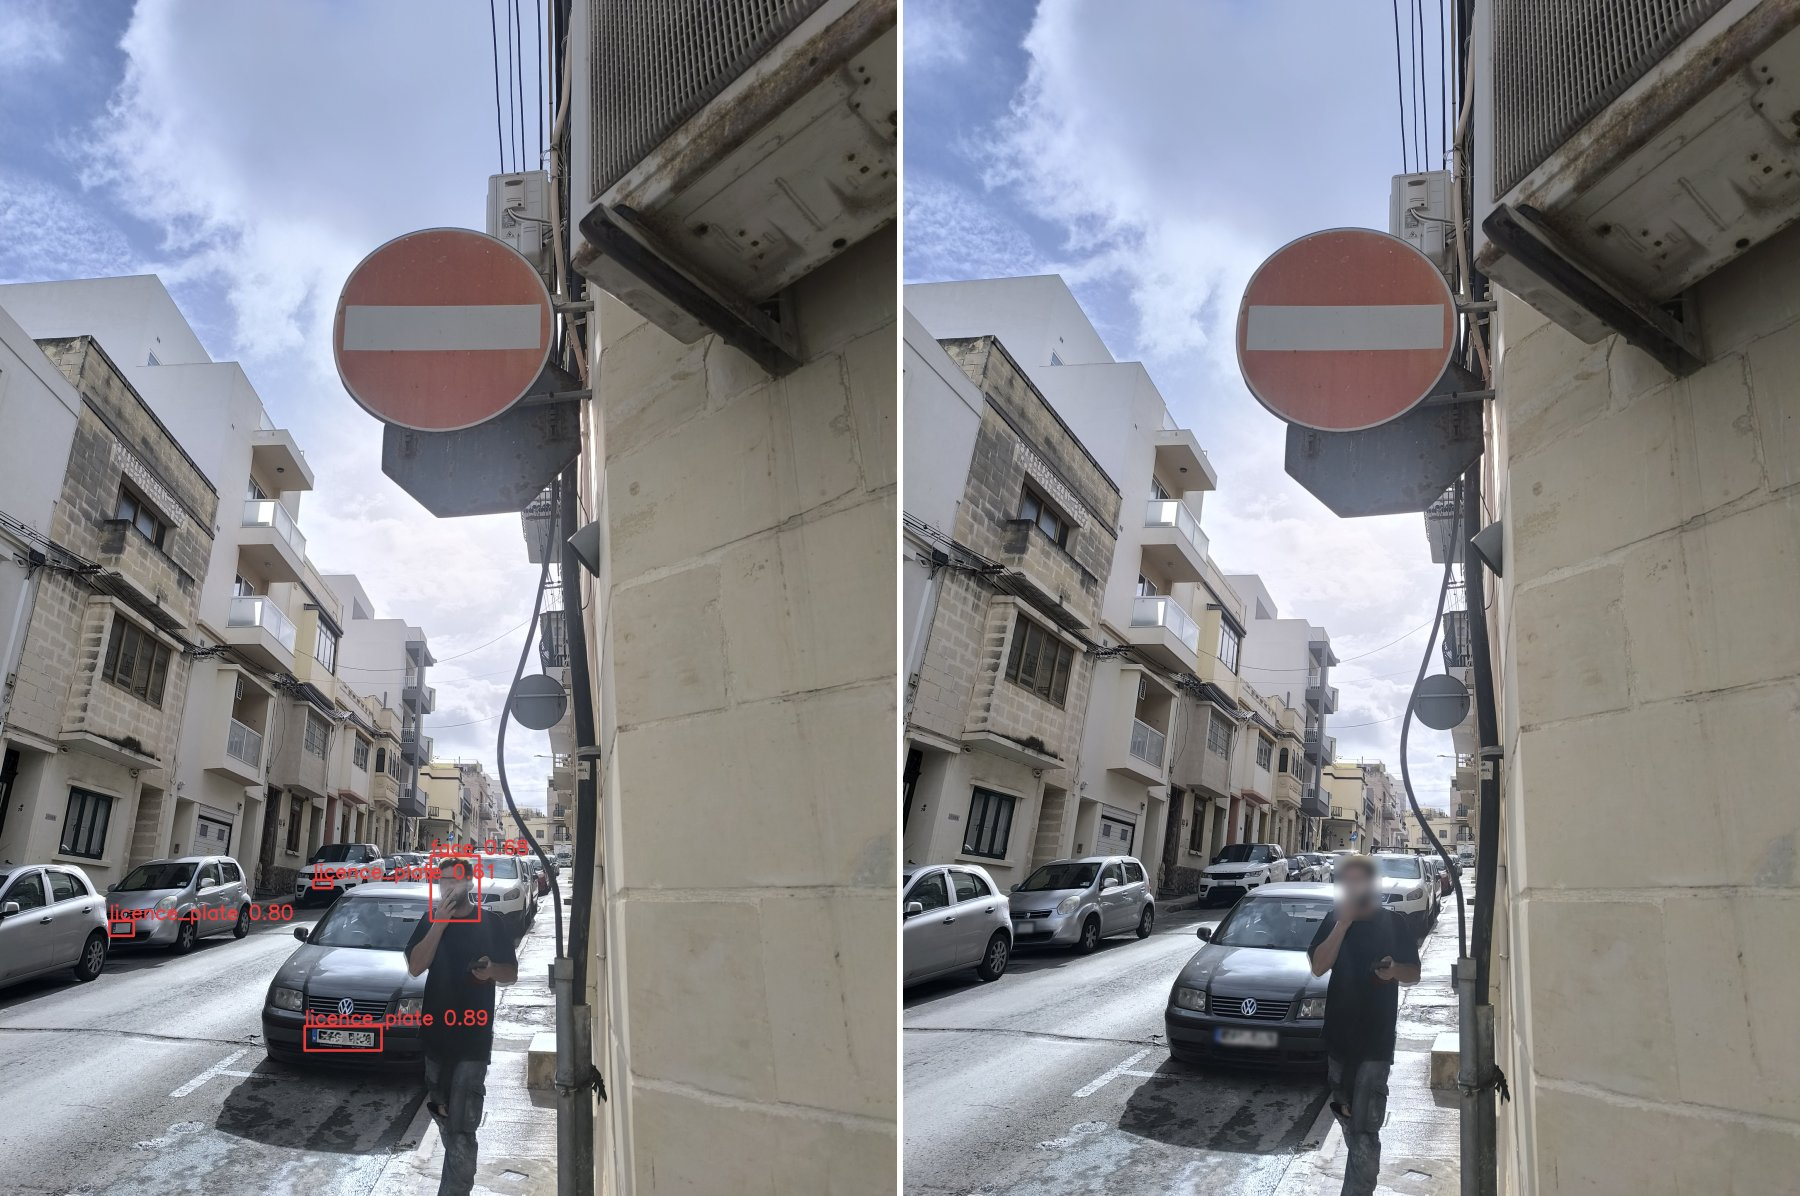
\includegraphics[width=\textwidth]{figures/Anonymization-1.jpg}
    \caption{Automated anonymisation using \gls{SAM} 3.1: predicted privacy regions (left) and the resulting blurred output (right). Faces and registration plates are AI-generated replacements and do not depict the original data.}
    \label{fig:anonymisation-example}
\end{figure}

\subsection{Annotation Procedure and Criteria}
\label{sec:md-annotation-protocol}
Following acquisition and anonymisation, the retained imagery was manually annotated by a team of professional annotators according to the taxonomies and operational definitions established in Chapter~\ref{ch:bg-lit}, supported throughout by dataset-specific guidance promoting consistent interpretation of object categories, inclusion criteria and, for the \gls{MTSD}, the associated object-level attributes. The complete annotation criteria and decision rules are provided in Appendices~\ref{app:mdwd-annotation-criteria} and~\ref{app:mtsd-annotation-criteria}. No model-generated or \gls{AI}-assisted annotations were used. Annotation workflows differed between the two datasets: the \gls{MDWD} was annotated using Roboflow\footnote{\url{https://roboflow.com}}, whereas the \gls{MTSD} was annotated using CVAT\footnote{\url{https://cvat.ai}}, exported in Pascal--VOC XML format, and subsequently consolidated and reviewed using a locally hosted Label Studio\footnote{\url{https://labelstud.io}} instance.

\begin{figure}[H]
    \centering
    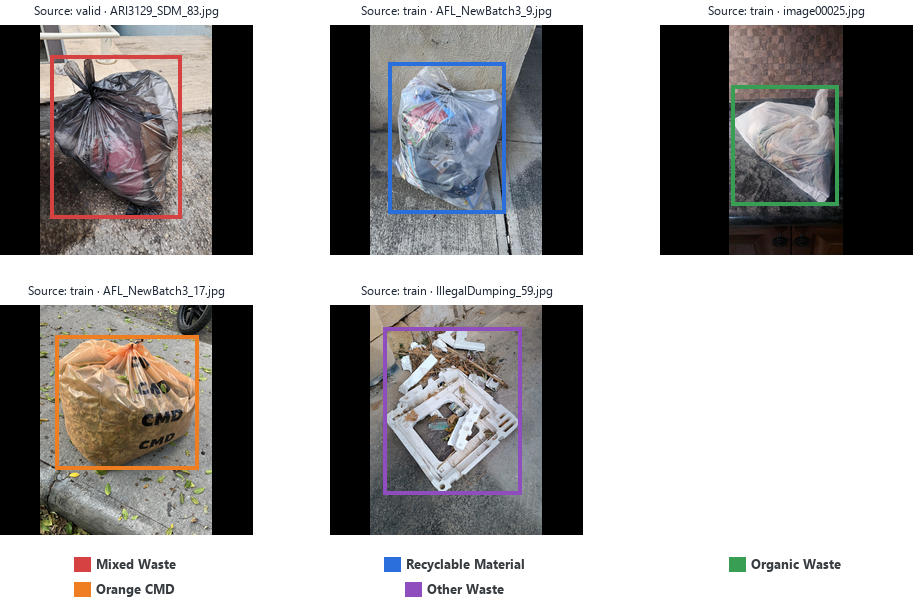
\includegraphics[width=\textwidth]{figures/mdwd_annotation_overview.png}
    \caption{Representative annotated samples illustrating the \gls{MDWD} taxonomy, with bounding-box colours indicating the corresponding waste categories.}
    \label{fig:mdwd-annotation-overview}
\end{figure}
\newpage
\noindent A common bounding-box convention was applied across both datasets, with each annotation tightly enclosing the visible extent of the corresponding object while excluding unrelated background wherever possible, as illustrated for the \gls{MDWD} in Figure~\ref{fig:mdwd-annotation-overview}. Partially occluded objects were retained where approximately \(20\%\) or more remained visible for reliable identification, with boxes restricted to the visible extent rather than extrapolated into occluded regions. Ambiguous or borderline cases were resolved through the review process described in Subsection~\ref{sec:md-annotation-qa}, and the small number of images containing no eligible target objects was retained as negative examples rather than removed from the source corpora.

Similarly, each eligible \gls{MTSD} object was represented by a single bounding box, assigned one traffic-sign category and one label for each of the four object-level attributes, so that all semantic and attribute annotations referred to the same localised instance, as illustrated in Figure~\ref{fig:mtsd-annotation-overview}. Objects were excluded where their identity or required attribute labels could not be established reliably, most commonly when distance, blur, occlusion or poor illumination prevented confident assessment of properties such as geometric shape or physical condition; such exclusions applied only to the affected object, with the surrounding image retained where other valid annotations were present. This avoided introducing uncertain or inferred labels into the \gls{GT} annotations while preserving otherwise usable imagery.

\begin{figure}[H]
    \centering
    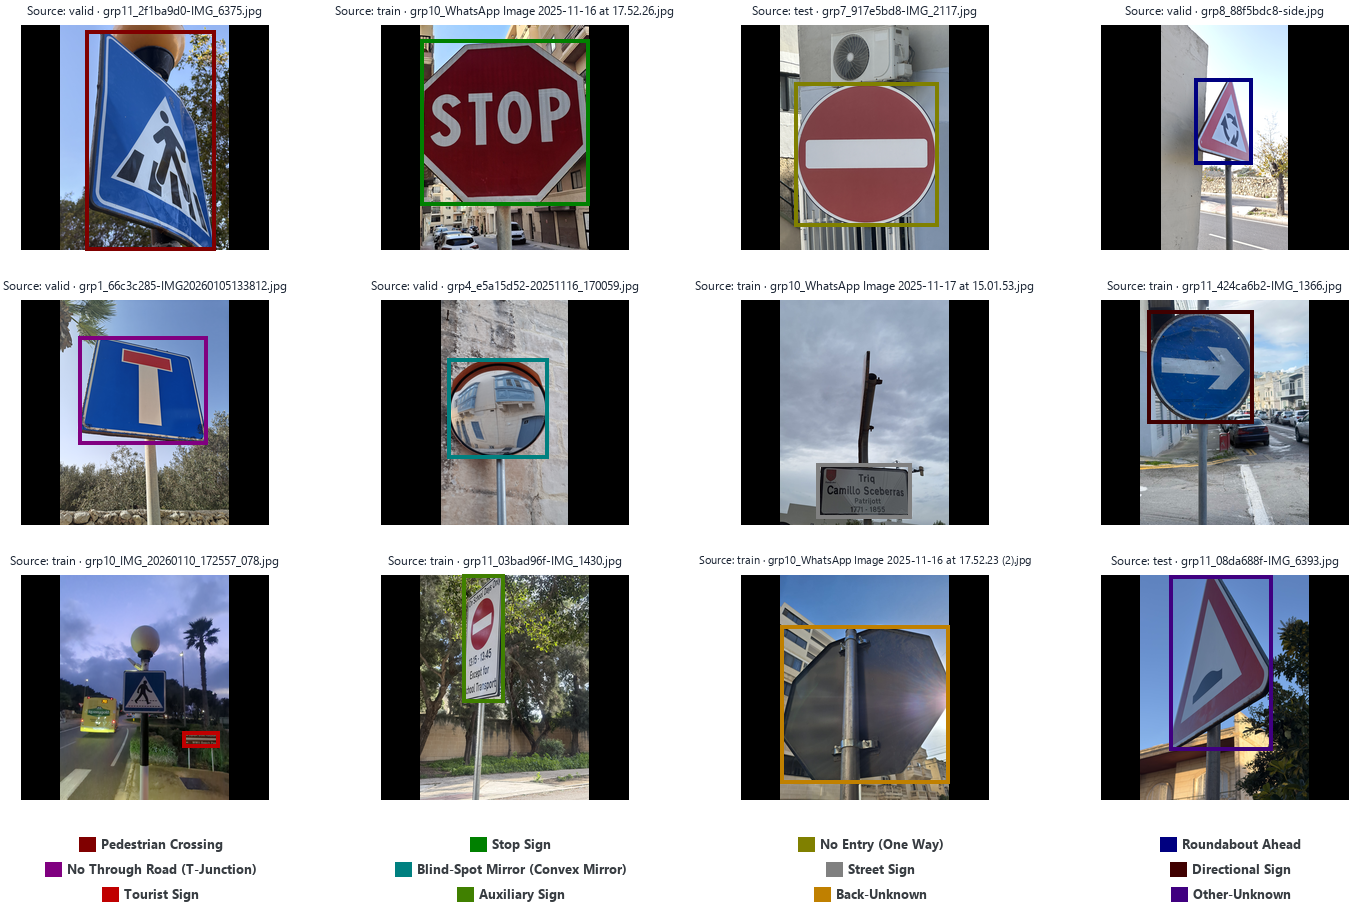
\includegraphics[width=\textwidth]{figures/mtsd_annotation_overview.png}
    \caption{Representative examples of \gls{MTSD} annotations, with one highlighted instance shown for each traffic-sign category.}
    \label{fig:mtsd-annotation-overview}
\end{figure}

\subsection{Annotation \gls{QA} and Agreement Stability Analysis}
\label{sec:md-annotation-qa}
Annotation quality was controlled through the staged review and adjudication workflow illustrated in Figure~\ref{fig:annotation-qa-workflow}, with the objective of establishing a consistent \gls{GT} standard across both datasets. Annotations produced by the annotation team were first examined by the review team and then assessed by the \gls{QA} lead. At this stage, annotations were either accepted as final \gls{GT}, corrected directly by the \gls{QA} lead, or returned to the annotation team where further revision was required. Returned annotations re-entered the workflow from the annotation stage and were reviewed again, with this iterative process continuing until all annotations satisfied the required \gls{QA} standard and were accepted as final \gls{GT}.

\begin{figure}[htbp]
    \centering
    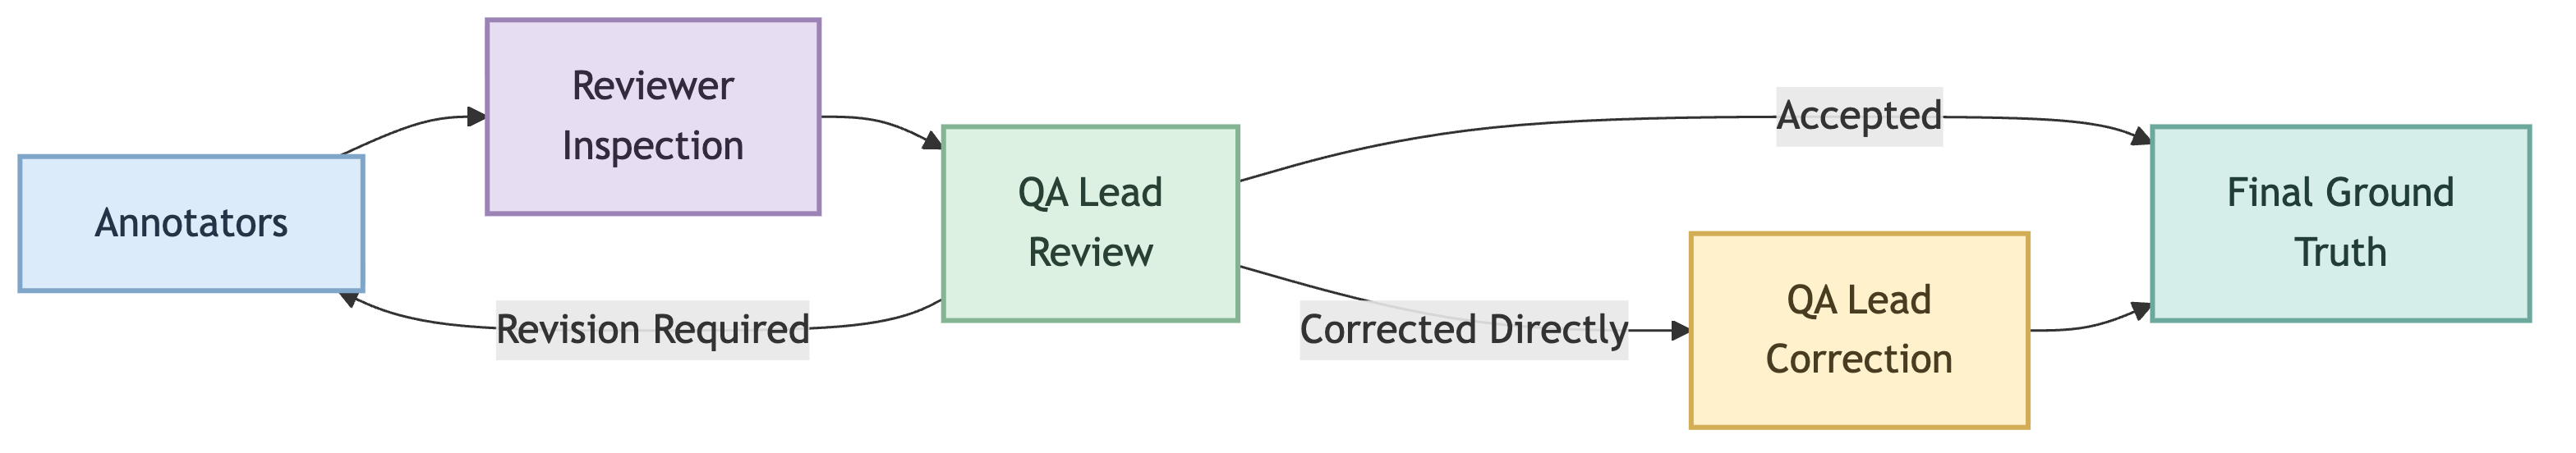
\includegraphics[width=\textwidth]{figures/QA-Workflow.png}
    \caption{Annotation \gls{QA} workflow used to establish the final ground-truth annotations.}
    \label{fig:annotation-qa-workflow}
\end{figure}

\noindent Agreement was quantified using Cohen's \(\kappa\) \cite{cohen1960coefficient} for categorical annotation fields and \gls{IoU} for bounding-box localisation, defined as:

\begin{equation}
\label{eq:kappa-iou}
\kappa = \frac{p_o-p_e}{1-p_e}, \qquad
\mathrm{IoU}(B_1,B_2) = \frac{|B_1\cap B_2|}{|B_1\cup B_2|},
\end{equation}

\noindent where \(p_o\) denotes the observed agreement, \(p_e\) the agreement expected by chance, and \(B_1\) and \(B_2\) the corresponding bounding boxes before and after review.

The versioned annotation history retained for the \gls{MTSD} enabled direct comparison between its initial and reviewed annotation states. Objects were paired within each image using greedy one-to-one matching based on maximum \gls{IoU}, irrespective of class label, with a minimum matching threshold of 0.50. This procedure identified 17,828 matched objects, while 2,681 objects were added and 196 removed during review. Across the matched objects, mean \gls{IoU} reached 0.99, indicating that bounding-box geometry remained highly consistent for instances retained between the two annotation states.

\newpage
\noindent Annotation completeness was considered separately from this geometric agreement. The 2,681 objects introduced during review represent approximately 13.07\% of the 20,509 annotations in the final \gls{MTSD}, indicating that initially omitted instances constituted a more substantial source of correction than bounding-box adjustment. Review also identified recurring revisions to object category, viewing angle and physical condition, together with occasional changes to bounding-box extent. Objects added or removed during review had no corresponding annotation against which agreement could be measured and were therefore excluded from both the mean \gls{IoU} and Cohen's \(\kappa\) calculations.

\begin{table}[h]
\centering
\caption{Agreement between the initial and reviewed \gls{MTSD} annotations for the 17,828 matched objects.}
\label{tab:mtsd-annotation-agreement}
\begin{tabular}{@{}lr@{}}
\toprule
    \textbf{Annotation field} & \textbf{Cohen's $\kappa$} \\
    \midrule
    Object class & 0.97 \\
    Viewing angle & 0.95 \\
    Mounting type & 0.96 \\
    Physical condition & 0.74 \\
    Geometric shape & 0.99 \\
\bottomrule
\end{tabular}
\end{table}

\noindent As shown in Table~\ref{tab:mtsd-annotation-agreement}, most categorical fields remained highly stable through review, with Cohen's \(\kappa\) values between 0.95 and 0.99. The revisions that did occur were concentrated mainly around less clearly defined cases, particularly oblique signs where the boundary between front, side and back views was more difficult to determine, together with occasional corrections between visually or semantically related sign categories. Physical condition exhibited the lowest stability, with a Cohen's \(\kappa\) of 0.74, reflecting the greater interpretative difficulty involved in assessing the severity of visible deterioration. Review frequently required clarification when distinguishing between \emph{Good}, \emph{Weathered} and \emph{Heavily Damaged} signs, particularly where rust, fading, stickers, scratches or minor surface markings were present. This comparatively higher level of revision is therefore taken into account when interpreting the subsequent attribute-classification results.

An equivalent quantitative comparison could not be reproduced for the \gls{MDWD} because its pre-review annotation state was not retained. Qualitative observations from its review process nevertheless indicated that corrections occurred primarily within dense groups of overlapping waste bags, where separating adjacent instances of similar appearance affected both instance identification and bounding-box placement. Some class ambiguity was also observed between recyclable and mixed-waste bags where illumination, discolouration or camera flash altered their apparent colour.

\subsection{Dataset Partitioning and Split Integrity}
\label{sec:md-partitioning}
To preserve independence between model development and evaluation, partitioning was performed at source-corpus level after annotation and \gls{QA}, but before augmentation or any other task-specific transformation. Each dataset was divided into fixed training, validation and test subsets in proportions of \textbf{80/10/10}, without class stratification, balancing or resampling, thereby retaining the naturally occurring class composition of each corpus. The \gls{MDWD} partition was generated once through Roboflow, while the \gls{MTSD} was partitioned deterministically using seed~42, with images sharing identical SHA-256 hashes constrained to the same subset to prevent byte-identical files from crossing partition boundaries. Once established, these source-image assignments were retained throughout the subsequent experiments, providing a consistent basis for training, model selection and final evaluation within each dataset.

\begin{figure}[H]
\centering
    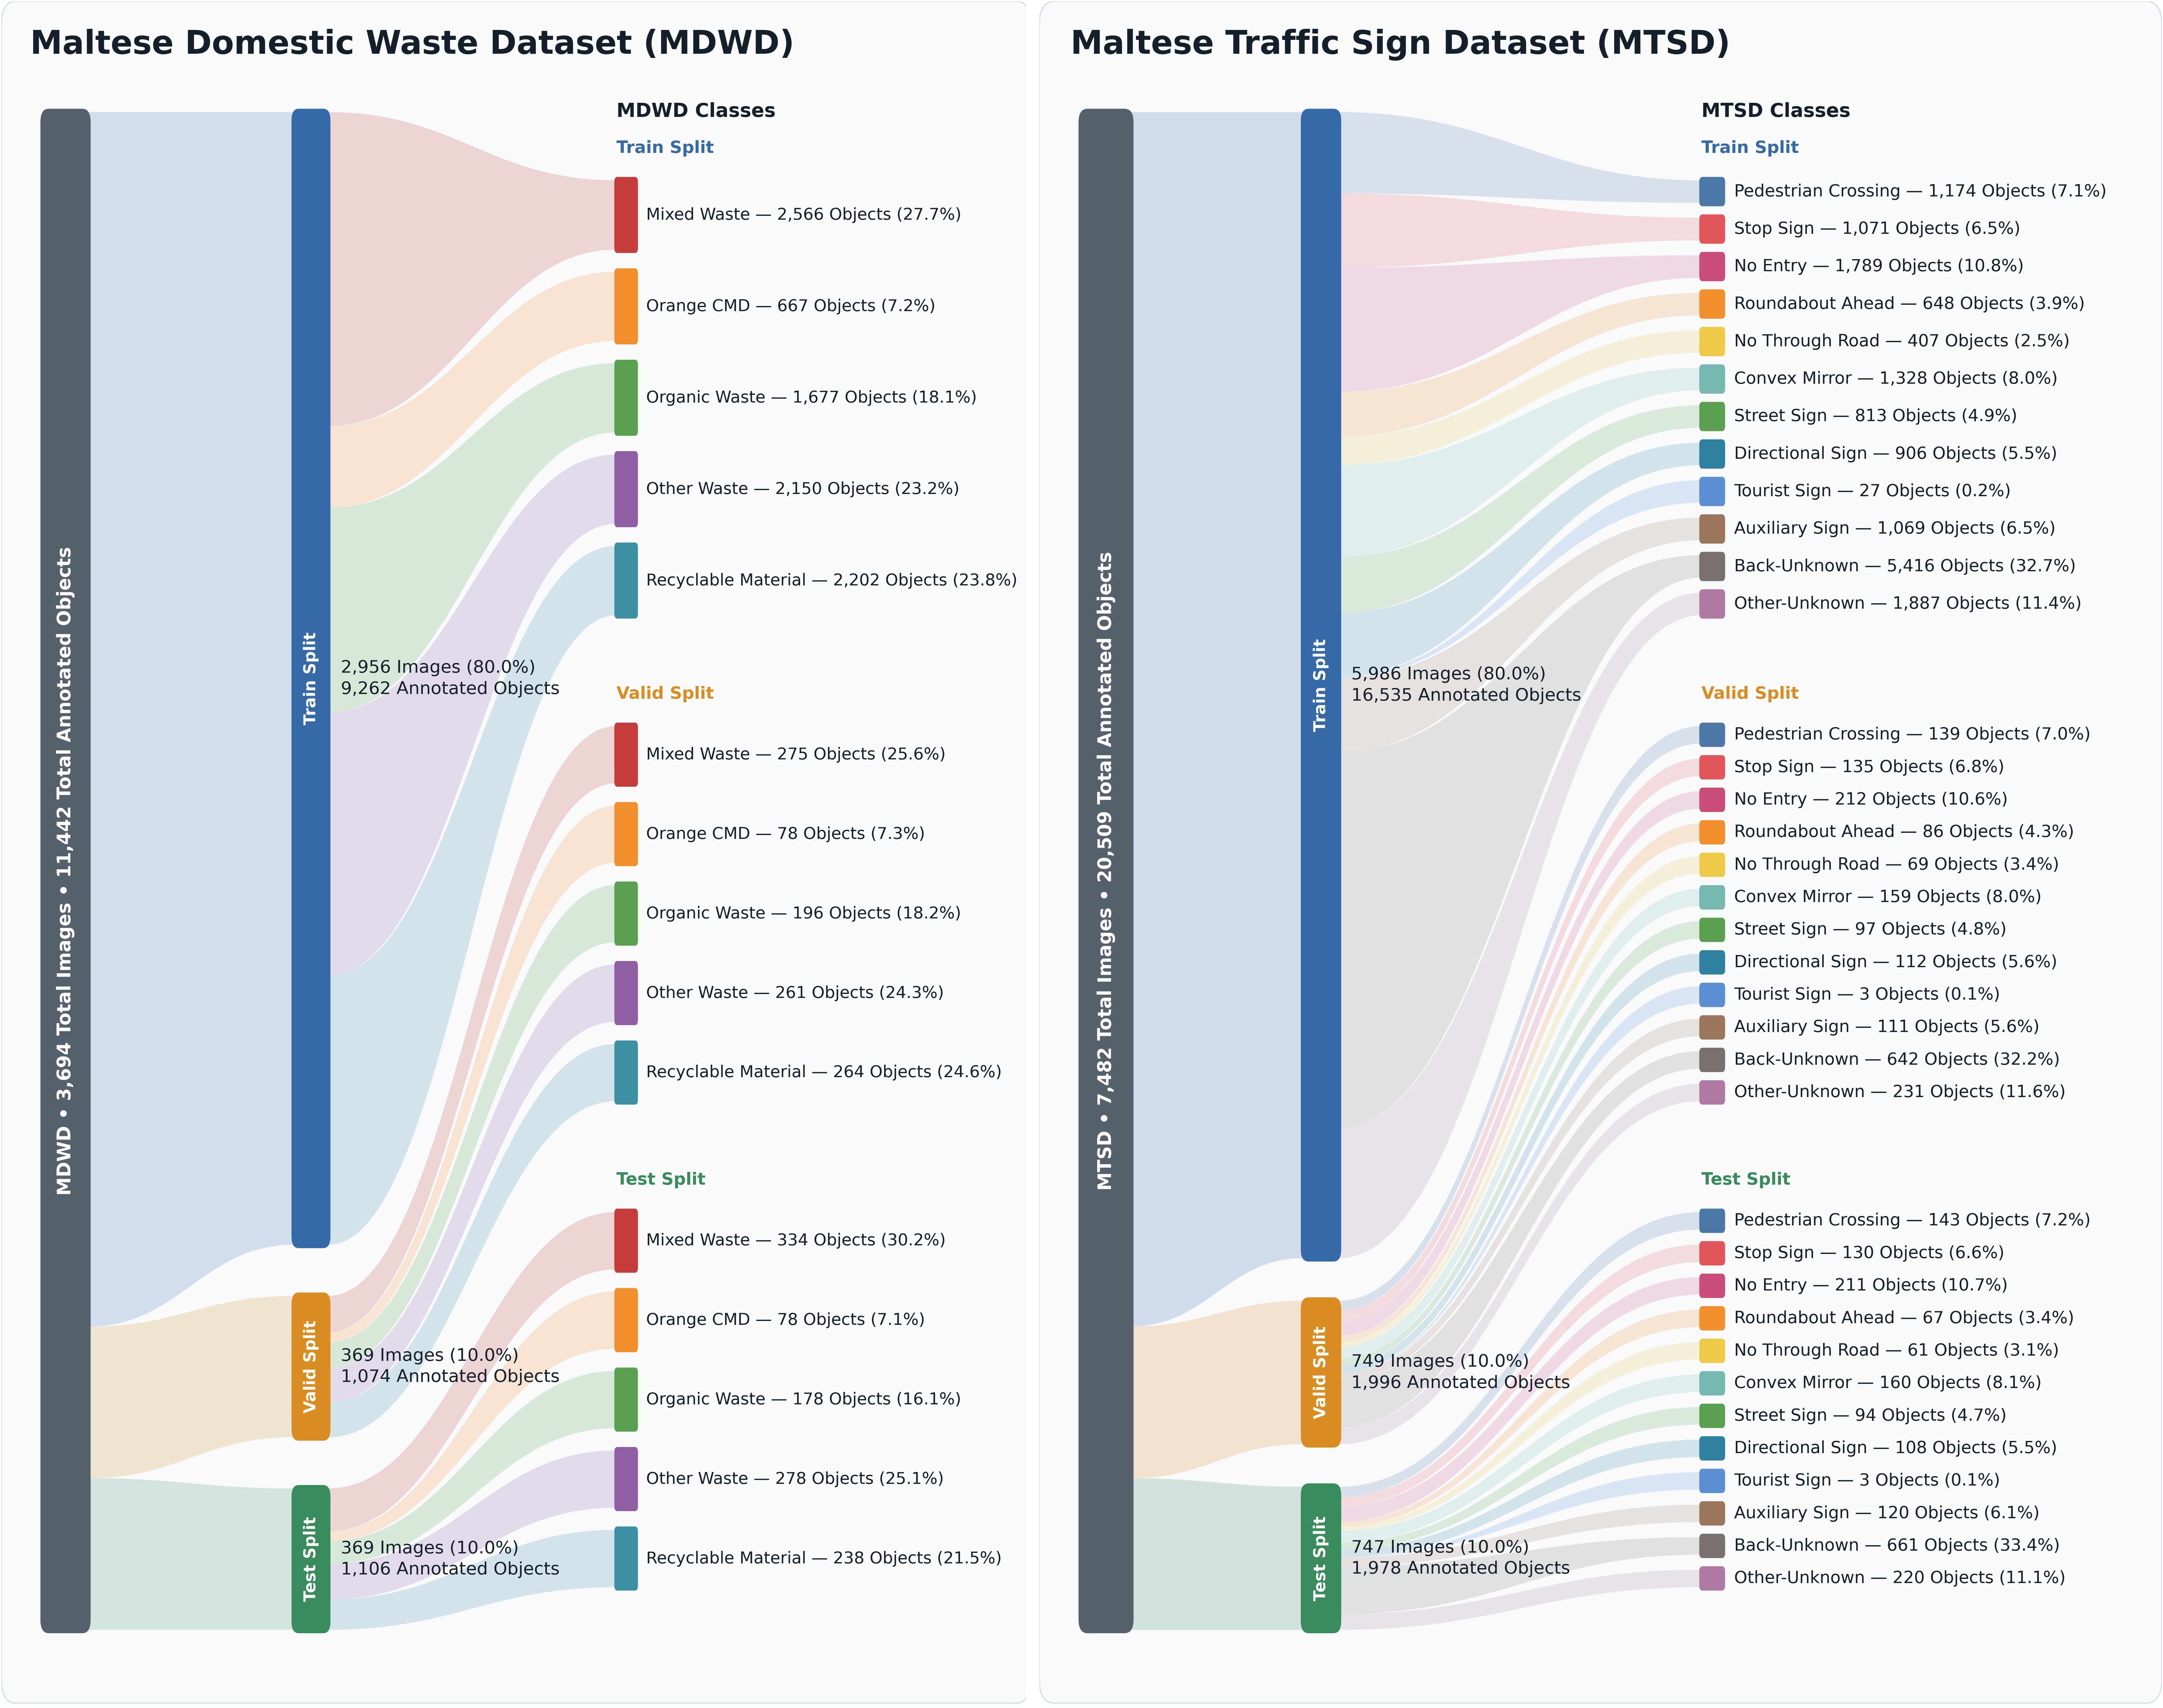
\includegraphics[width=\textwidth]{figures/MDWD-MTSD-Breakdown.png}
    \caption{Training, validation and test partitioning of the \gls{MDWD} and \gls{MTSD}, together with the corresponding class distributions within each split.}
    \label{fig:mdwd-mtsd-breakdown}
\end{figure}

\newpage
\noindent The resulting partition and class distributions, illustrated in Figure~\ref{fig:mdwd-mtsd-breakdown}, show that \gls{MDWD} class proportions remain broadly consistent across the three subsets, varying by less than two percentage points. \emph{Other Waste} is among the more frequently represented categories, reflecting its deliberately heterogeneous scope and inclusion of waste that does not conform to the principal bag-based collection streams. Conversely, \emph{Orange \gls{CMD}} is the least represented class, consistent with the less frequent occurrence of \gls{CMD} cleansing activity relative to routine household waste presentation. Its distinctive colour and presentation nevertheless provide comparatively strong visual separation from the remaining waste categories despite the smaller number of annotated instances.

Greater class imbalance is evident within the \gls{MTSD}, although this arises largely from the structure of the annotation taxonomy rather than from the partitioning procedure itself. \emph{Back-Unknown} constitutes the largest class because conventional traffic signs observed from the rear were assigned to this category whenever their frontal semantic identity could not be established from the available visual evidence. This decision avoided assigning semantic classes through contextual inference or requiring the model to distinguish between sign types that are visually indistinguishable from the rear. Roadside assets whose identity remained recoverable from their physical form, such as convex mirrors and directional bollards, retained their corresponding semantic class irrespective of viewing direction. The prevalence of \emph{Back-Unknown} therefore reflects both the frequency of rear-facing observations and the deliberate treatment of semantic ambiguity within the taxonomy. 

\emph{Other-Unknown} is similarly broad by design, grouping signs outside the explicitly modelled categories rather than fragmenting them into numerous sparsely represented classes. The remaining semantic categories are distributed more consistently across the three partitions, although \emph{Roundabout Ahead} and \emph{No Through Road} show greater proportional variation because of their comparatively small sample sizes.

A further distinction between the source and experiment-ready \gls{MTSD} taxonomies concerns the \emph{Tourist Sign} class. Only 33 instances were present in the source corpus, comprising 27 training, three validation and three test examples, which was considered insufficient for meaningful supervised learning or reliable class-specific evaluation given the visual variability of the category. Its annotations were therefore excluded from the experiment-ready target taxonomy used for supervised detection and zero-shot localisation. The corresponding bounding boxes were retained as ignore regions during localisation evaluation, such that predictions overlapping a Tourist Sign instance were excluded from true-positive and false-positive assignment rather than treated as background errors. This ensured that the class was neither learned nor evaluated as a modelled category while preventing valid localisation of an otherwise recognisable traffic sign from being penalised.

\newpage
\subsection{Exploratory Dataset Analysis (\gls{EDA})}
\label{sec:eda}
The \gls{EDA} was conducted on the final \gls{QA}-approved source annotations to characterise properties of the two datasets likely to influence the subsequent learning tasks, considering object scale, bounding-box geometry and scene density across both corpora, together with \gls{MDWD} class co-occurrence and the distribution of \gls{MTSD} object-level attributes and their association with semantic class. These statistics are calculated across the complete 20,509-instance \gls{MTSD} source corpus, including the 33 \emph{Tourist Sign} instances retained at this stage.

\begin{table}[H]
    \centering
    \caption{Object-scale, bounding-box geometry, and density statistics for both datasets. Relative area denotes bounding-box area as a percentage of the corresponding source-image area.}
    \label{tab:eda-comparison}

    \renewcommand{\arraystretch}{1.15}
    \begin{tabularx}{\textwidth}{@{}Xrr@{}}
        \toprule
        \textbf{Statistic}
        & \textbf{\gls{MDWD}}
        & \textbf{\gls{MTSD}} \\
        \midrule

        \multicolumn{3}{@{}l}{\textit{Object scale}} \\[2pt]
        Relative area, median
            & 2.52\% & 0.94\% \\
        Relative area, Q1--Q3
            & 0.90--5.85\% & 0.03--6.08\% \\
        Objects below 0.1\% of frame
            & 5.81\% & 36.05\% \\

        \midrule
        \multicolumn{3}{@{}l}{\textit{Bounding-box geometry}} \\[2pt]
        Aspect ratio, median
            & 1.00 & 0.91 \\
        Aspect ratio, Q1--Q3
            & 0.80--1.26 & 0.56--1.08 \\

        \midrule
        \multicolumn{3}{@{}l}{\textit{Object density}} \\[2pt]
        Objects per image, mean
            & 3.10 & 2.74 \\
        Objects per image, median
            & 2 & 2 \\
        Objects in busiest image
            & 34 & 24 \\

        \bottomrule
    \end{tabularx}
\end{table}

\noindent As summarised in Table~\ref{tab:eda-comparison}, \gls{MDWD} objects generally occupy a larger proportion of the source image, with a median relative bounding-box area of 2.52\%, compared with 0.94\% for the \gls{MTSD}. The contrast is more pronounced among very small instances, with 36.05\% of \gls{MTSD} objects occupying less than 0.1\% of the source frame, compared with 5.81\% in the \gls{MDWD}. Object density is more comparable between the datasets, averaging 3.10 and 2.74 annotated instances per image, respectively, while the wider interquartile range of \gls{MTSD} aspect ratios reflects greater variation in the geometry of the annotated roadside assets.

\begin{table}[H]
\centering
\caption{Per-class object-scale characteristics for the \gls{MDWD} and \gls{MTSD}. Relative area is expressed as a percentage of the corresponding source-image area.}
\label{tab:eda-class-scale}
\renewcommand{\arraystretch}{1.12}
\small
\begin{tabularx}{\textwidth}{@{}Xrrrr@{}}
\toprule
\textbf{Class} & \textbf{Instances} & \textbf{Q1 (\%)} & \textbf{Median (\%)} & \textbf{$<0.1\%$} \\
\midrule

\multicolumn{5}{@{}l}{\textit{\gls{MDWD}}} \\[2pt]
Mixed Waste             & 3,175 & 1.22 & 3.14 & 2.68\% \\
Orange \gls{CMD}        & 823   & 0.22 & 1.42 & 19.20\% \\
Organic Waste           & 2,051 & 0.88 & 1.84 & 3.46\% \\
Other Waste             & 2,689 & 0.39 & 1.68 & 9.93\% \\
Recyclable Material     & 2,704 & 1.64 & 4.19 & 3.11\% \\

\midrule
\multicolumn{5}{@{}l}{\textit{\gls{MTSD}}} \\[2pt]
Pedestrian Crossing                 & 1,456 & 0.03 & 1.22 & 37.02\% \\
Stop Sign                           & 1,336 & 0.74 & 3.77 & 15.87\% \\
No Entry (One Way)                  & 2,212 & 0.06 & 2.53 & 28.57\% \\
Roundabout Ahead                    & 801   & 0.06 & 3.07 & 29.09\% \\
No Through Road (T-Junction)        & 537   & 2.11 & 4.75 & 7.08\% \\
Blind-Spot Mirror (Convex Mirror)   & 1,647 & 0.40 & 3.88 & 17.30\% \\
Street Sign                         & 1,004 & 0.03 & 0.26 & 41.04\% \\
Directional Sign                    & 1,126 & 0.02 & 0.05 & 62.79\% \\
Tourist Sign                        & 33    & 0.05 & 1.21 & 27.27\% \\
Auxiliary Sign                      & 1,300 & 0.01 & 0.07 & 54.46\% \\
Back-Unknown                        & 6,719 & 0.03 & 0.87 & 37.37\% \\
Other-Unknown                       & 2,338 & 0.02 & 0.13 & 47.35\% \\

\bottomrule
\end{tabularx}
\end{table}

\noindent Considerable variation is also present between semantic classes, as shown in Table~\ref{tab:eda-class-scale}. Within the \gls{MDWD}, \emph{Orange \gls{CMD}} is the smallest category in image space, with a median relative area of 1.42\% and 19.20\% of instances below 0.1\% of the frame. The \gls{MTSD} exhibits substantially greater class-dependent variation: \emph{Directional Sign} has a median relative area of only 0.05\%, with 62.79\% of instances below the 0.1\% threshold, while \emph{Auxiliary Sign}, \emph{Other-Unknown} and \emph{Street Sign} likewise contain particularly high proportions of very small objects. By contrast, classes such as \emph{No Through Road} and \emph{Stop Sign} are typically represented at substantially larger image scales.

\newpage
\noindent Since camera-to-object distance is unavailable within the annotations, relative bounding-box area is used as an image-space proxy for object scale rather than an estimate of physical distance. This provides one basis for interpreting later model behaviour, particularly within the \gls{MTSD}, where the prevalence and class dependence of small objects motivate the input-resolution experiment in Section~\ref{subsec:mtsd-augmentation-resolution}. A complementary source of difficulty arises from the way classes co-occur within individual scenes. Within the \gls{MDWD}, the strongest off-diagonal co-occurrence is observed between \emph{Other Waste} and \emph{Recyclable Material}, which appear together in 589 images, corresponding to 15.94\% of the source corpus. Given the heterogeneous scope of \emph{Other Waste}, this frequent co-occurrence indicates that the detector is often required to distinguish visually competing categories within the same scene. Together, these scale- and context-related characteristics provide the basis for the subsequent robustness analysis in Section~\ref{sec:robustness-error-analysis}.

The four \gls{MTSD} attributes exhibit markedly different class distributions, as illustrated in Figure~\ref{fig:mtsd-attribute-distribution}. Viewing angle is comparatively balanced, whereas mounting type and physical condition are dominated by \emph{Pole-Mounted} and \emph{Good} instances, respectively. Geometric shape is also unevenly distributed, with \emph{Circular} and \emph{Quadrangle} accounting for the majority of annotations and \emph{Pentagon} represented only sparsely. All 20,509 source-corpus instances contain a valid label for each of the four attributes, so this imbalance reflects differences in class prevalence rather than missing supervision.

\begin{figure}[H]
    \centering
    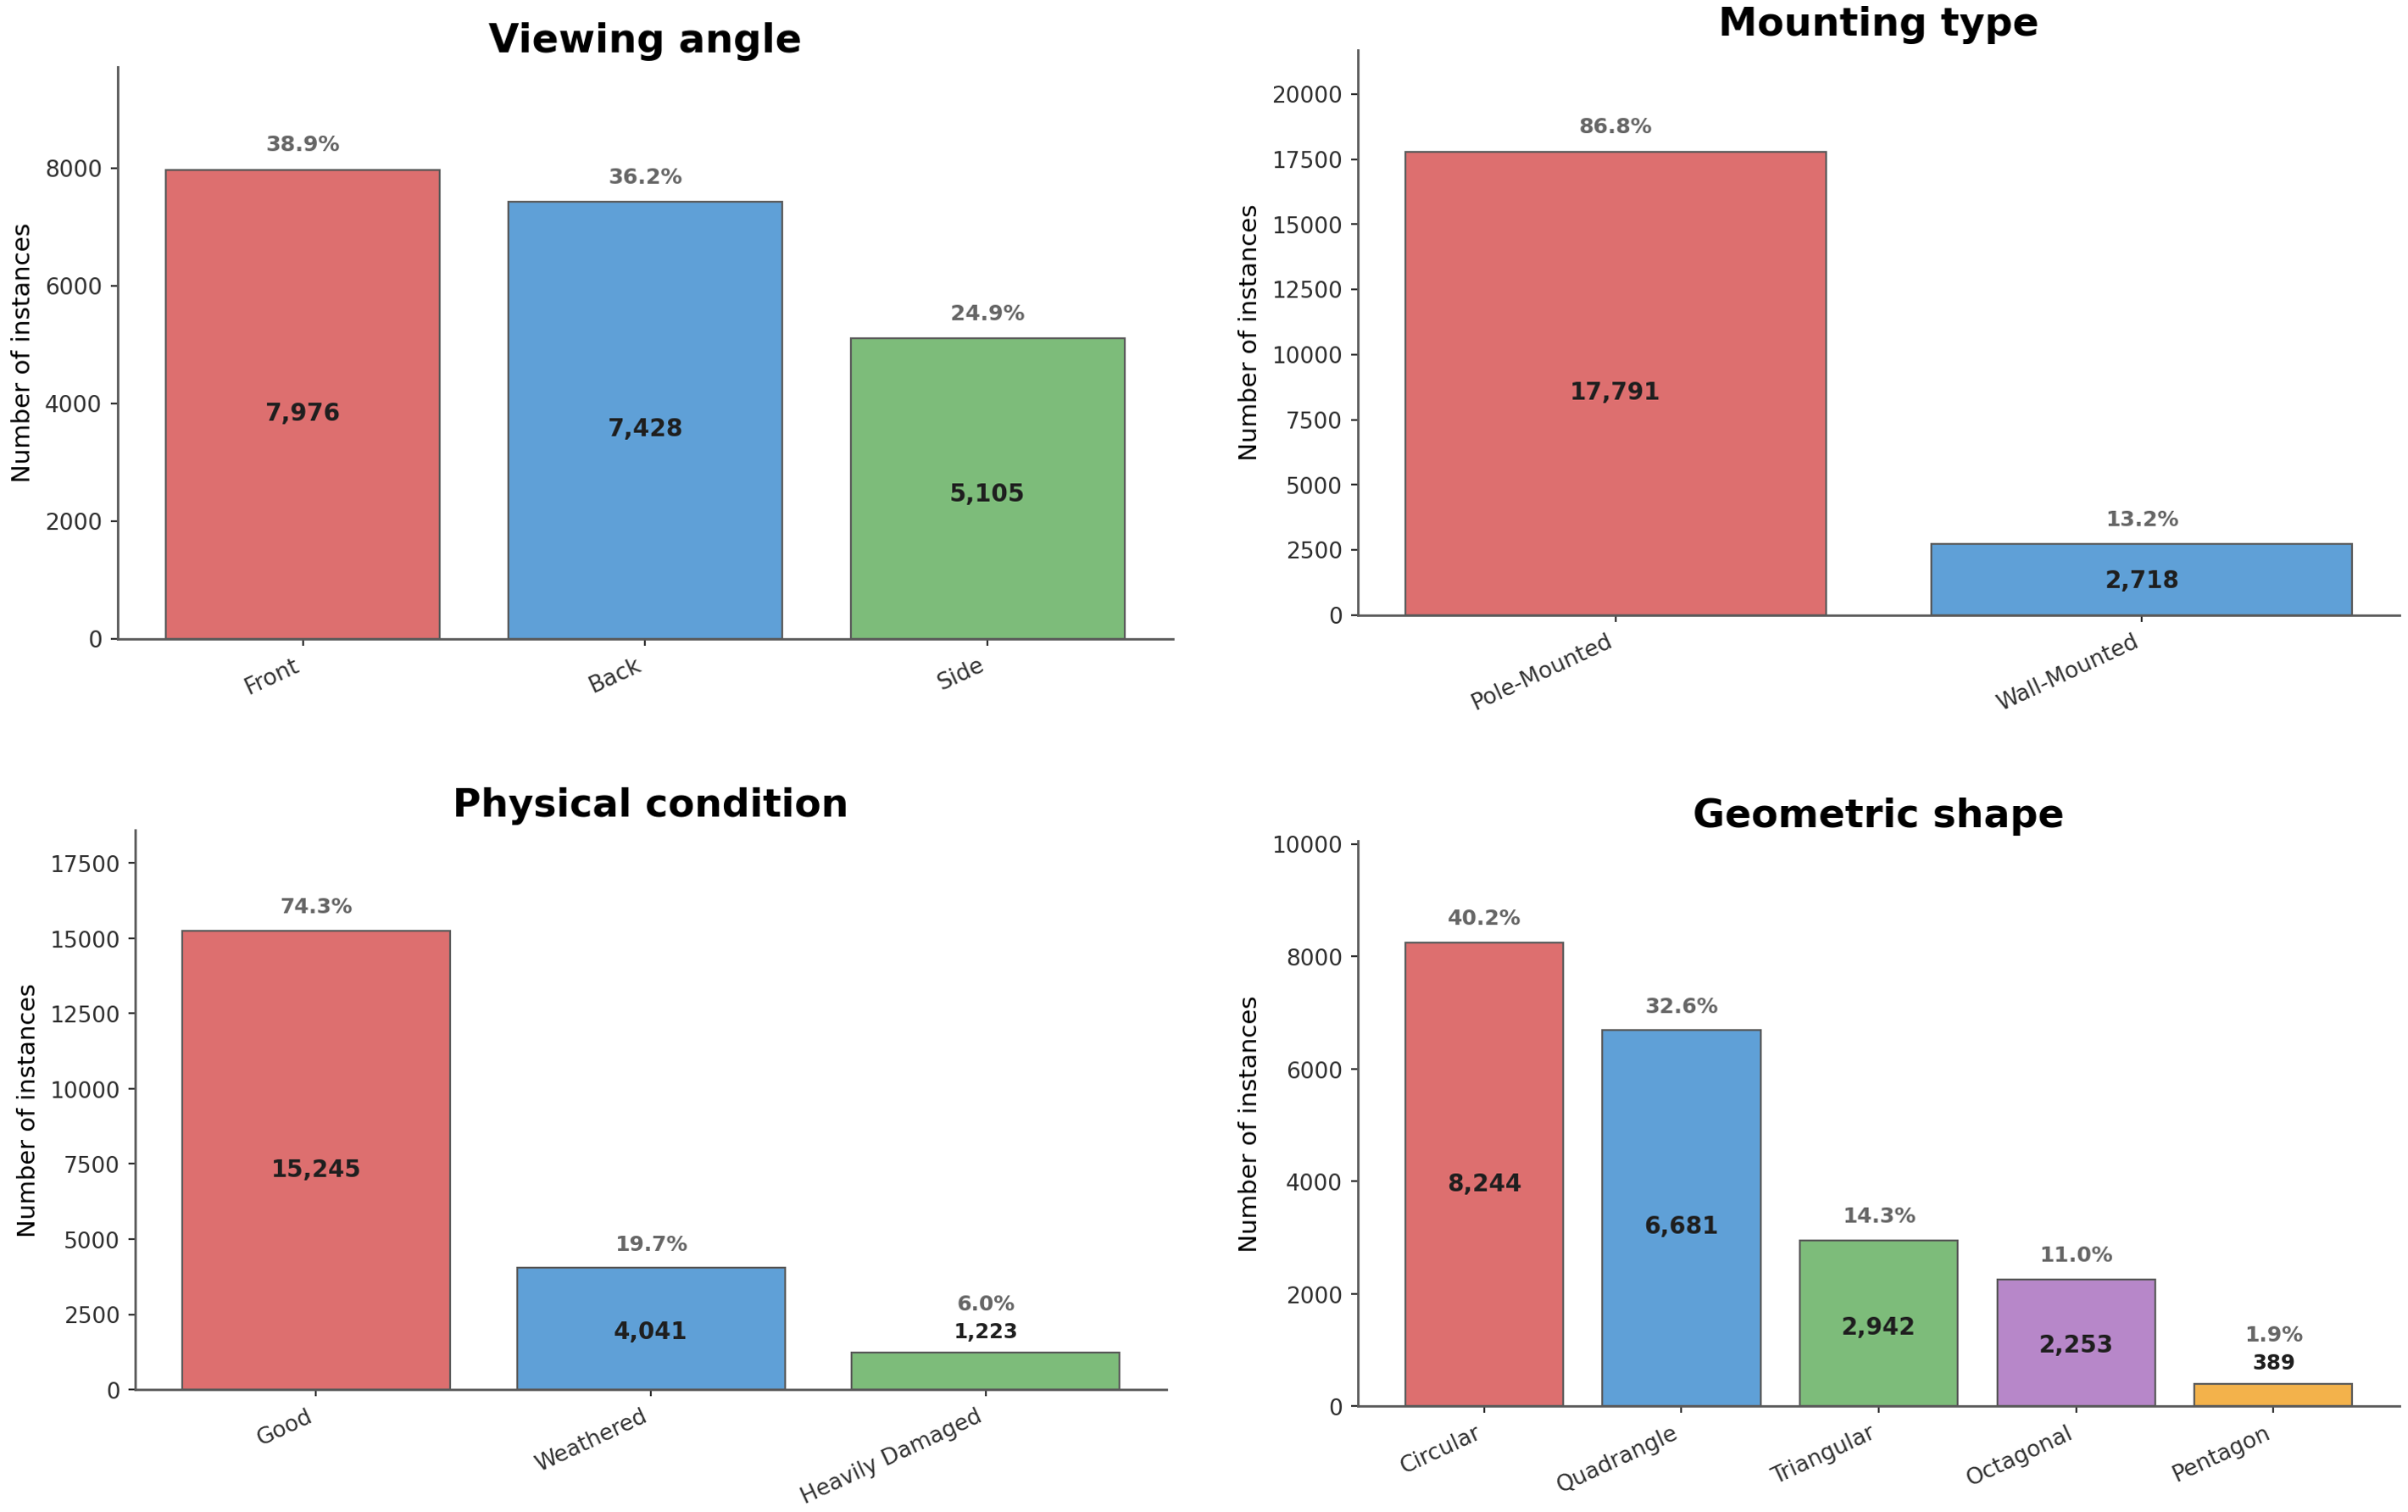
\includegraphics[width=\textwidth]{figures/MTSD_AttributeDistribution.png}
    \caption{Distribution of the four traffic-sign attributes across the 20,509 annotated instances.}
    \label{fig:mtsd-attribute-distribution}
\end{figure}

\noindent Associations between semantic object class and the four \gls{MTSD} attributes were quantified using Cramér's \(V\), which measures association between categorical variables from Pearson's \(\chi^2\) statistic~\cite{cramers}. For a contingency table with \(r\) rows, \(c\) columns and \(n\) observations,

\begin{equation}
\label{eq:cramers-v}
V = \sqrt{\frac{\chi^2}{n\,\min(r-1,c-1)}}.
\end{equation}

\noindent Values range from \(0\), indicating no association, towards \(1\) as association strengthens. Although conventional Cramér's \(V\) can exhibit positive finite-sample bias~\cite{bergsma}, this effect is expected to be limited given the size of the \gls{MTSD} relative to the contingency tables considered. The values are therefore interpreted primarily in terms of relative association strength. As shown in Table~\ref{tab:mtsd-class-attribute-association}, viewing angle and geometric shape exhibit the strongest associations with semantic class, with Cramér's \(V\) values of 0.67 and 0.62, respectively. This reflects the taxonomy, particularly the strong correspondence between \emph{Back-Unknown} and the \emph{Back} viewing-angle label, together with characteristic geometric forms associated with several sign classes. Mounting type shows a moderate association (\(V=0.49\)), driven particularly by the predominance of wall-mounted \emph{Street Sign} instances, while physical condition is only weakly associated with semantic class (\(V=0.14\)).

\begin{table}[H]
\centering
\caption{Association between \gls{MTSD} semantic object class and each object-level attribute, measured using Cramér's \(V\).}
\label{tab:mtsd-class-attribute-association}
\renewcommand{\arraystretch}{1.4}
\setlength{\tabcolsep}{6pt}
\begin{tabularx}{\textwidth}{
    @{}
    >{\raggedright\arraybackslash}p{3.2cm}
    @{\hspace{0.6cm}}
    >{\raggedright\arraybackslash}p{2.2cm}
    @{\hspace{0.6cm}}
    >{\raggedright\arraybackslash}X
    @{}
}
\toprule
\textbf{Attribute} & \textbf{Cramér's \(V\)} & \textbf{Principal association} \\
\midrule
Viewing angle      & 0.67 & \emph{Back-Unknown} strongly associated with \emph{Back} \\
Mounting type      & 0.49 & \emph{Street Sign} predominantly wall-mounted \\
Physical condition & 0.14 & Weak association with semantic class \\
Geometric shape    & 0.62 & Strong class-specific geometric structure \\
\bottomrule
\end{tabularx}
\end{table}

\noindent These relationships are relevant to the subsequent attribute-classification experiments, since some attributes may be predicted partly from cues associated with semantic identity, while physical condition depends more directly on the observed state of the individual asset. Attribute imbalance is therefore considered through overall accuracy, macro-averaged \(F_1\) and per-class measures.

\subsection{Experimental Data Preparation and Augmentation}
\label{sec:md-training-data-prep}
Following the source-image partitioning defined in Subsection~\ref{sec:md-partitioning}, data preparation was performed separately for each experimental track while preserving validation and test independence. Augmentation was restricted to the training data, with held-out images receiving only model-specific deterministic preprocessing. The \gls{MDWD} detection experiments used a fixed offline augmentation pipeline, whereas the \gls{MTSD} detection experiments compared three augmentation strategies. Attribute classification employed a separate crop-based pipeline with online training augmentation.

\subsubsection{\gls{MDWD} Detection Data Preparation and Augmentation}
\label{sec:md-augmentation-mdwd}
The \gls{MDWD} imagery was first normalised to a consistent orientation and subsequently resized to \(640 \times 640\) pixels using stretch-based resizing. Preliminary resolution trials produced only marginal differences in validation performance across the tested input sizes, indicating that the standard \(640 \times 640\) configuration provided an appropriate balance between predictive performance and computational cost. This resolution was therefore retained as the fixed reference input size for all \gls{MDWD} detector experiments, ensuring that all models were trained and evaluated under a common spatial configuration.

Stretch-based resizing was selected in preference to letterboxing to avoid introducing padding that could interact with the subsequent mosaic augmentation process. Because the source imagery is predominantly portrait-oriented, resizing directly to a square input alters the original aspect ratio and introduces anisotropic geometric distortion. However, this transformation was applied consistently across the complete \gls{MDWD} and was therefore treated as part of the standardised experimental representation rather than as a source of variation between detector configurations.

Offline augmentation was generated once using Roboflow and reused across all \gls{MDWD} detector experiments to ensure a consistent training corpus. Ten outputs were produced per source training image, consisting of the resized original and nine augmented derivatives, increasing the effective training set to 29,580 images. Generating the augmented corpus in advance ensured that each detector was exposed to the same transformed samples, supporting a fair comparison across architectures. All augmentation was restricted to the training partition, while validation and test imagery remained unchanged apart from the required deterministic preprocessing. The applied transformations and their respective configurations are summarised in Table~\ref{tab:mdwd-augmentation}.

\begin{table}[H]
  \caption{Offline augmentation configuration applied to the \gls{MDWD} training partition through Roboflow.}
  \label{tab:mdwd-augmentation}
  \centering
  \begin{tabular*}{\columnwidth}{@{\extracolsep{\fill}}lr@{}}
    \toprule
    \textbf{Augmentation} & \textbf{Configuration} \\
    \midrule
    Resize                & $640 \times 640$ (Stretch) \\
    Horizontal Flip       & 50\% probability \\
    Vertical Flip         & 50\% probability \\
    Hue Adjustment        & $\pm 19^{\circ}$ \\
    Saturation Adjustment & $\pm 29\%$ \\
    Brightness Adjustment & $\pm 17\%$ \\
    Exposure Adjustment   & $\pm 10\%$ \\
    Gaussian Blur         & Up to 1\,px \\
    Motion Blur           & Up to 40\,px \\
    Mosaic Augmentation   & Enabled ($2{\times}2$) \\
    \bottomrule
  \end{tabular*}
\end{table}

\noindent The selected transformations were chosen to reflect variation expected during street-level image acquisition, with representative augmented samples shown in Figure~\ref{fig:mdwd-augmentation-examples}. Photometric augmentation broadens variation in illumination, colour and image response, while Gaussian and motion blur simulate degradation associated with imperfect focus and camera or vehicle movement. Mosaic augmentation further increases diversity in surrounding context, apparent object scale and spatial arrangement by combining multiple training images into a single composite sample.

\begin{figure}[H]
    \centering
    \makebox[\textwidth][c]{%
        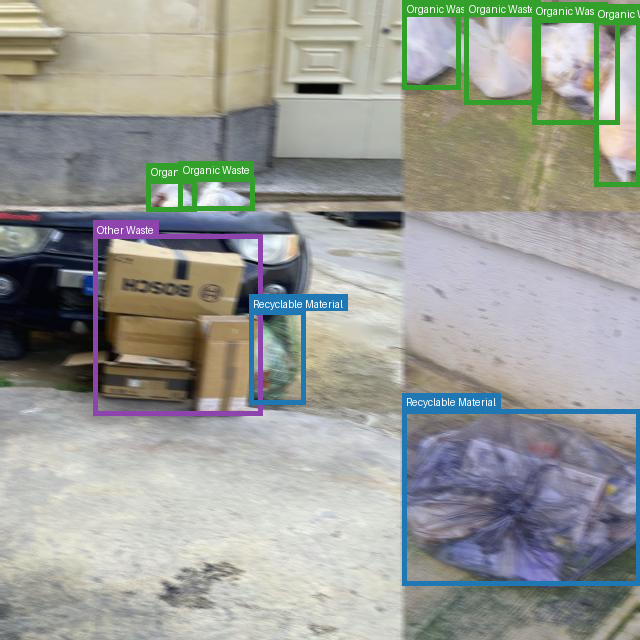
\includegraphics[width=0.5\textwidth]{figures/MDWD-Aug-1.jpg}%
        \hspace{0.02\textwidth}%
        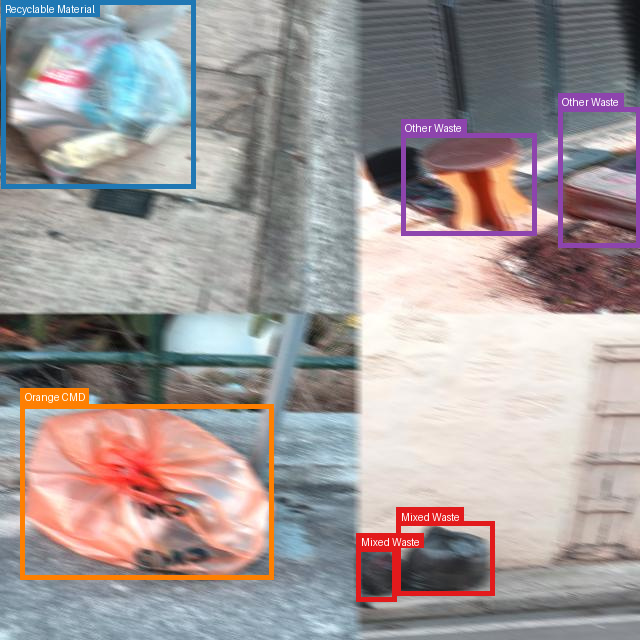
\includegraphics[width=0.5\textwidth]{figures/MDWD-Aug-2.jpg}%
    }
    \caption{Two representative examples of the final augmented \gls{MDWD} training images supplied to the detection models, illustrating the combined augmentation pipeline with overlaid bounding boxes denoting annotated \gls{MSW} instances.}
    \label{fig:mdwd-augmentation-examples}
\end{figure}

\newpage
\noindent Horizontal reflection was retained as a conventional augmentation for street-level imagery, while vertical reflection was included specifically for the \gls{MDWD} due to the less constrained orientation of deformable waste objects, which may topple, collapse or otherwise appear in irregular configurations. Motion blur of up to 40 pixels was also applied to reflect acquisition artefacts observed in imagery captured from slowly moving vehicles. Although comparatively aggressive, this transformation was retained because preliminary validation indicated improved generalisation.

\subsubsection{\gls{MTSD} Detection Augmentation Strategies}
\label{sec:md-augmentation-mtsd}
To examine the effect of training-data variation on \gls{MTSD} detection performance, three alternative augmentation strategies were defined: \emph{none}, \emph{mild} and \emph{strong}. All three operate from the same fixed source-image partitions, comprising 5,986 training, 749 validation and 747 test images, so that the experimental conditions differ in their training representations rather than their underlying data allocation. The \emph{none} strategy provides the unaugmented reference condition using the original \gls{QA}-approved imagery, while \emph{mild} and \emph{strong} each generate four outputs per source training image, consisting of the original and three augmented derivatives, expanding the training set from 5,986 to 23,944 images. The two strategies progressively increase the degree of visual variation presented during training, as illustrated comparatively in Figure~\ref{fig:mtsd-augmentation-examples}.

\begin{figure}[H]
    \centering
    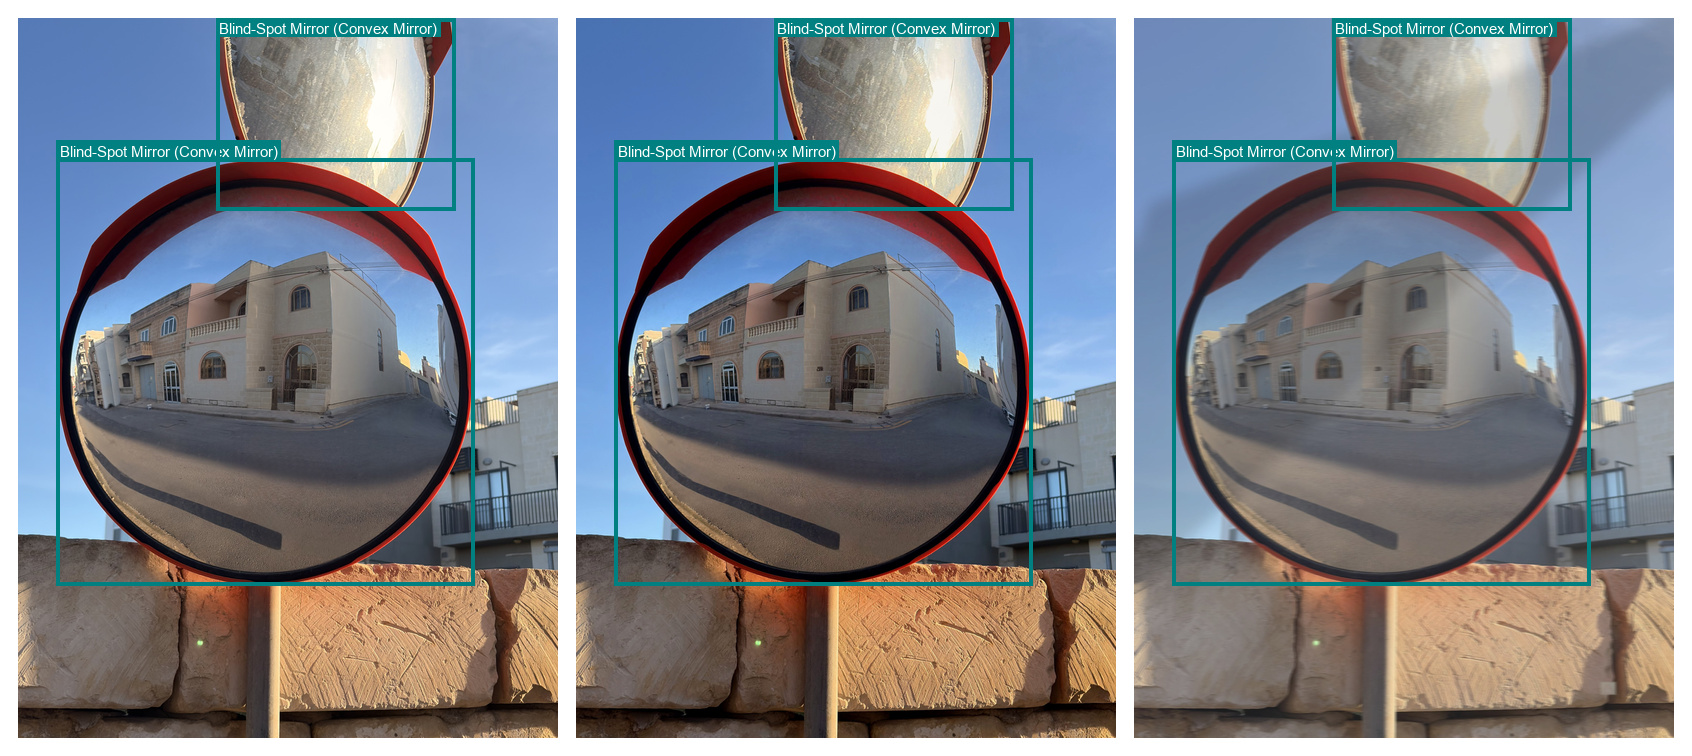
\includegraphics[width=\textwidth]{figures/MTSD-Aug-1.jpg}
    \caption{Representative \gls{MTSD} sample under the three augmentation strategies: \emph{none} (left), \emph{mild} (centre) and \emph{strong} (right), illustrating the progressively greater photometric and geometric variation introduced by each strategy.}
    \label{fig:mtsd-augmentation-examples}
\end{figure}

\newpage
\noindent The \emph{mild} strategy was designed to preserve object geometry and bounding-box coordinates while introducing limited photometric and acquisition-related variation. The transformation ranges reported in Table~\ref{tab:mtsd-augmentation} were therefore selected to produce modest departures from the source imagery, broadening visual appearance without substantially altering the spatial characteristics of the traffic signs.

By contrast, the \emph{strong} strategy introduces broader geometric and scene-level variation, including changes to object position, scale, orientation and perspective, together with more substantial modifications to illumination and scene composition. Where a transformation alters object geometry or visibility, the associated bounding boxes are recalculated, clipped to the visible image region and filtered according to the criteria in Table~\ref{tab:mtsd-augmentation}. The strategy was designed to expose detectors to a wider range of plausible viewing and acquisition conditions while preserving the semantic identity of the underlying traffic sign.

\begin{table}[h]
\centering
\caption{Offline augmentation configurations for the \emph{mild} and \emph{strong} \gls{MTSD} strategies.}
\label{tab:mtsd-augmentation}

\normalsize
\renewcommand{\arraystretch}{1.04}
\setlength{\tabcolsep}{4pt}

\begin{tabularx}{\textwidth}{
    @{}
    >{\raggedright\arraybackslash}p{3.4cm}
    >{\raggedright\arraybackslash}p{4.3cm}
    >{\raggedright\arraybackslash}X
    @{}
}
\toprule
\textbf{Transformation} & \textbf{Mild} & \textbf{Strong} \\
\midrule

Brightness
& \(0.80\)--\(1.20\)
& \(75\%\), \(0.65\)--\(1.35\) \\

Contrast
& \(0.85\)--\(1.15\)
& \(75\%\), \(0.70\)--\(1.30\) \\

Saturation
& \(0.90\)--\(1.10\)
& \(70\%\), \(0.80\)--\(1.20\) \\

Gamma
& \(0.90\)--\(1.10\)
& \(70\%\), \(0.70\)--\(1.35\) \\

\addlinespace[0.15em]

Gaussian blur
& \(50\%\), \(\sigma \leq 1.0\)
& \(50\%\), \(\sigma \leq 1.5\) \\

Gaussian noise
& \(30\%\), \(\sigma \leq 0.02\)
& \(50\%\), \(\sigma \leq 0.04\) \\

JPEG compression
& \(30\%\), quality \(70\)--\(92\)
& \(60\%\), quality \(45\)--\(90\) \\

Motion blur
& Horizontal \(9\)-px kernel, weight \(0.85\)
& \(35\%\), kernel \(\{7,9,11\}\) px \\

\addlinespace[0.15em]

Illumination effects
& --
& Shadow \(25\%\); gradient \(25\%\); local \(20\%\); haze \(15\%\) \\

Translation
& --
& Up to \(10\%\) width/height \\

Scale
& --
& \(0.75\)--\(1.30\) \\

Rotation
& --
& \(-5^{\circ}\) to \(+5^{\circ}\) \\

Shear
& --
& Up to \(2^{\circ}\) \\

Perspective
& --
& Distortion \(0.02\) \\

Random crop
& --
& \(35\%\); retained-box visibility \(\geq 85\%\) \\

\addlinespace[0.15em]

Mosaic
& --
& \(40\%\); \(1280 \times 1280\); centre \(40\%\)--\(60\%\) \\

Rare-class copy-paste
& --
& \(20\%\); up to 2 instances; scale \(0.80\)--\(1.25\); max.\ \gls{IoU} \(0.20\) \\

\addlinespace[0.15em]

Bounding-box handling
& Coordinates unchanged
& Recomputed and filtered: visibility \(\geq 35\%\), dimensions \(\geq 2\) px, area \(\geq 9\) px \\

\midrule

\textbf{Training-set size}
& \textbf{23,944 images}
& \textbf{23,944 images} \\

\bottomrule
\end{tabularx}
\end{table}

\newpage
\noindent To complement this broader augmentation strategy, rare-class copy-paste was applied to increase the representation of underrepresented modelled categories, particularly \emph{Roundabout Ahead} and \emph{No Through Road}. Up to two annotated instances were inserted subject to predefined scale and overlap constraints, with source identity, placement coordinates and resulting bounding boxes recorded in the augmentation manifest for reproducibility. Consequently, the \emph{strong} strategy modifies not only the visual diversity of the training data, but also its effective class distribution, as quantified in Table~\ref{tab:mtsd-augmentation-class-balance}.

\begin{table}[H]
\centering
\caption{Effective \gls{MTSD} training-instance counts under the three augmentation strategies.}
\label{tab:mtsd-augmentation-class-balance}
\small
\begin{tabularx}{\textwidth}{@{}Xrrr@{}}
\toprule
\textbf{Class} & \textbf{None} & \textbf{Mild} & \textbf{Strong} \\
\midrule
Pedestrian Crossing & 1,174 & 4,696 & 8,635 \\
Stop Sign & 1,071 & 4,284 & 7,998 \\
No Entry (One Way) & 1,789 & 7,156 & 13,048 \\
Roundabout Ahead & 648 & 2,592 & 6,519 \\
No Through Road (T-Junction) & 407 & 1,628 & 4,827 \\
Blind-Spot Mirror (Convex Mirror) & 1,328 & 5,312 & 9,863 \\
Street Sign & 813 & 3,252 & 5,823 \\
Directional Sign & 906 & 3,624 & 6,296 \\
Auxiliary Sign & 1,069 & 4,276 & 7,562 \\
Back-Unknown & 5,416 & 21,664 & 39,519 \\
Other-Unknown & 1,887 & 7,548 & 13,624 \\
\midrule
\textbf{Modelled total} & \textbf{16,508} & \textbf{66,032} & \textbf{123,714} \\
\bottomrule
\end{tabularx}
\end{table}

\noindent Across the 11 modelled classes, the majority-to-minority ratio remains unchanged at 13.31 under the \emph{none} and \emph{mild} strategies, but decreases to 8.19 under \emph{strong}. The corresponding coefficient of variation also falls from 0.87 to 0.83, indicating a modest reduction in overall class-frequency dispersion. Horizontal reflection was excluded because it may alter semantically meaningful sign orientation, while MixUp was omitted because translucent composites were considered unrepresentative of plausible street-level observations. All offline augmentation was generated deterministically from seed~42, source-image identity and derivative index, ensuring that the experiment-ready corpora can be reproduced consistently.

The three conditions are therefore treated as complete training-data strategies rather than as a single-factor augmentation ablation. They differ in both the extent of introduced variation and the resulting training exposure, with the \emph{strong} strategy additionally affecting object geometry, scene composition and class balance. Subsequent performance differences are consequently interpreted at the strategy level rather than attributed to individual transformations.

\subsubsection{Attribute-Crop Generation and Online Augmentation}
\label{sec:md-augmentation-attribute}
Attribute classification uses an object-centred representation derived directly from the \gls{GT} annotations of the \gls{MTSD}. Each annotated instance was extracted with a \(25\%\) contextual margin around its bounding box, retaining limited surrounding scene information that may support interpretation of attributes such as mounting type and viewing angle, and square-padded with neutral grey rather than geometrically stretched, preserving the sign's original proportions prior to model-specific resizing and normalisation. Figure~\ref{fig:mtsd-attribute-crop-preparation} illustrates this preparation process, from the annotated source image through contextual expansion to the resulting square-padded model input. A single crop was generated per annotated instance, with no offline augmentation applied during crop generation.

\begin{figure}[H]
    \centering
    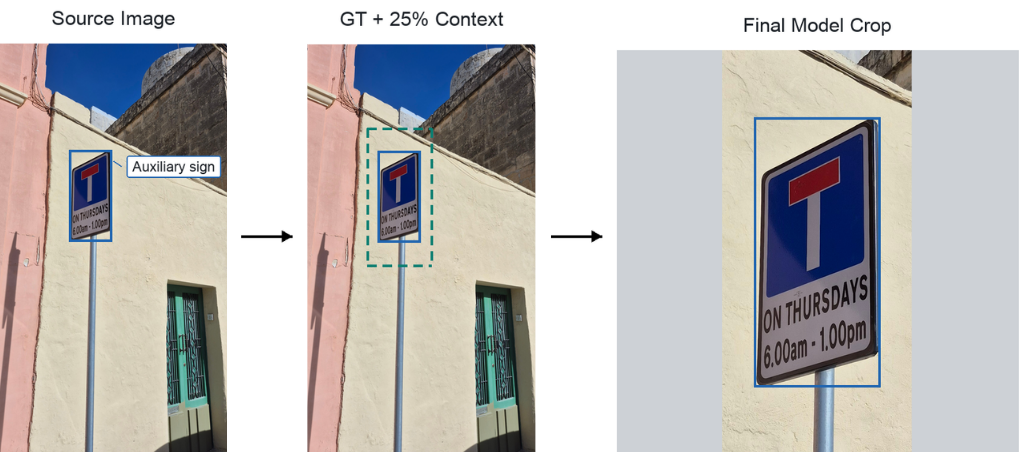
\includegraphics[width=\textwidth]{figures/MTSD-AttrCls.png}
    \caption{Attribute-crop preparation from the \gls{MTSD} source imagery, showing the \gls{GT} object localisation, \(25\%\) contextual expansion and square-padded model input.}
    \label{fig:mtsd-attribute-crop-preparation}
\end{figure}

\noindent Rather than generating additional crop variants offline, augmentation was applied dynamically to training crops only, while validation and test crops followed a fixed, deterministic pipeline. Training crops were first square-padded with the neutral-grey fill value \((114,114,114)\) and randomly rotated within \(\pm10^\circ\), with regions exposed by rotation filled with the same neutral grey. A \texttt{RandomResizedCrop} then sampled \(80\text{--}100\%\) of the padded area at an aspect ratio of \(0.90\text{--}1.11\), resizing the result to the backbone-specific resolution with antialiasing. Colour jitter was applied last, perturbing brightness and contrast by up to \(0.3\), saturation by up to \(0.2\), and hue by up to \(0.02\), before tensor conversion and ImageNet normalisation. Horizontal reflection was deliberately excluded, as it may alter orientation-dependent cues relevant to sign content and viewing angle, and no other transformations were applied. Validation and test crops, by contrast, underwent only square padding, antialiased resizing, tensor conversion and normalisation, with no rotation, cropping or colour perturbation, ensuring a consistent and reproducible evaluation input.

\newpage 
\section{Supervised Object Detection (\gls{OD})} 
\label{sec:supervised-detection-methodology}
The supervised detection study compares \gls{YOLO}11, \gls{YOLO}12, \gls{YOLO}26 and \gls{RF-DETR} across both the \gls{MDWD} and \gls{MTSD}, following the architectural rationale established in Section~\ref{sec:bg-supervised-od}. The methodology focuses on how detector family, model scale, training-data strategy and input resolution influence predictive performance and computational requirements under a common experimental framework. Each configuration was trained and evaluated using fixed dataset partitions, with task-specific weights learned independently for the two municipal domains. The following subsections define the model-scale comparisons, pretrained initialisation, shared training configuration and the additional augmentation and resolution experiments conducted on the \gls{MTSD}.

\subsection{Model-Scale Experiments}
\label{sec:supervised-model-ablation}
Each detector family was evaluated across multiple model scales to examine how increasing model capacity influences both predictive performance and computational demand. The principal comparison comprises the Nano (-N), Small (-S) and Medium (-M) variants of \gls{YOLO}11, \gls{YOLO}12, \gls{YOLO}26 and \gls{RF-DETR}, with the Large (-L) configuration additionally included for \gls{YOLO}26. Collectively, these variants form the 13 detector configurations summarised in Table~\ref{tab:model-matrix}.

Each configuration was trained independently on the \gls{MDWD} and \gls{MTSD}, with no transfer of task-specific weights between domains. Fixed dataset partitions were retained throughout so that within-dataset differences between model families and scales were assessed against an identical held-out test set.

\begin{table}[htbp]
\centering
\caption{Supervised detector families and model scales evaluated on the \gls{MDWD} and \gls{MTSD}. Parameter counts refer to the corresponding published pretrained detection checkpoints and are reported in millions of parameters.}
\label{tab:model-matrix}
\renewcommand{\arraystretch}{1.16}
\small
\begin{tabularx}{\textwidth}{
@{}
>{\raggedright\arraybackslash}p{2.1cm}
>{\raggedright\arraybackslash}X
>{\centering\arraybackslash}p{1.25cm}
>{\centering\arraybackslash}p{1.25cm}
>{\centering\arraybackslash}p{1.25cm}
>{\centering\arraybackslash}p{1.25cm}
@{}
}
\toprule
\textbf{Family} & \textbf{Architectural emphasis} & \textbf{N} & \textbf{S} & \textbf{M} & \textbf{L} \\
\midrule
\multicolumn{6}{@{}l}{\textit{\gls{YOLO}-based detectors}} \\
\addlinespace[0.2em]
    \gls{YOLO}11 & Efficiency-oriented \gls{YOLO} baseline & 2.6\,M & 9.4\,M & 20.1\,M & -- \\
    \gls{YOLO}12 & Attention-centric \gls{YOLO} & 2.6\,M & 9.3\,M & 20.2\,M & -- \\
    \gls{YOLO}26 & End-to-end, edge-oriented \gls{YOLO} & 2.4\,M & 9.5\,M & 20.4\,M & 24.8\,M \\
    \midrule
    \multicolumn{6}{@{}l}{\textit{Detection transformer}} \\
    \addlinespace[0.2em]
    \gls{RF-DETR} & \gls{DINO}v2-based detection transformer & 30.5\,M & 32.1\,M & 33.7\,M & -- \\
\bottomrule
\end{tabularx}
\end{table}

\newpage
\noindent Within each family, the -N variant represents the lowest-capacity configuration, while the -S and -M variants progressively increase model capacity at the cost of additional memory and computation. Comparing these scales therefore indicates whether increased capacity produces corresponding improvements in predictive performance or begins to yield diminishing returns. The \gls{YOLO}26-L configuration is not intended as a common scale across families, but is used specifically to examine whether this newest, deployment-oriented \gls{YOLO} architecture continues to benefit from increased capacity beyond -M.

The scale designations are interpreted within each detector family rather than as equivalent parameter budgets across architectures. For example, \gls{RF-DETR}-N contains substantially more parameters than the corresponding \gls{YOLO}-N models, while the increase in parameter count between its -N and -M variants is considerably smaller. The within-family comparisons therefore form the model-capacity analysis, while comparisons between detector families are treated as practical architecture-level comparisons rather than parameter-matched experiments.

\subsection{Pretrained Initialisation and Training Provenance}
\label{sec:supervised-pretraining-provenance}
All supervised detectors were fine-tuned from pretrained weights rather than trained from random initialisation. Checkpoint provenance is reported explicitly because differences in upstream pretraining form part of the conditions under which the resulting models are compared. Table~\ref{tab:detector-pretraining} summarises the initialisation checkpoint, pretraining provenance and training environment used for each configuration.

\begin{table}[htbp]
\centering
\caption{Pretrained initialisation and training provenance of the supervised detector configurations.}
\label{tab:detector-pretraining}
\renewcommand{\arraystretch}{1.25}
\small
\begin{tabularx}{\textwidth}{ @{}
>{\raggedright\arraybackslash}p{1.6cm}
>{\raggedright\arraybackslash}p{3.8cm}
>{\raggedright\arraybackslash}p{2.4cm}
>{\raggedright\arraybackslash}X
>{\raggedright\arraybackslash}p{2.4cm} @{} }
\toprule
\textbf{Family} & \textbf{Initialisation checkpoint} & \textbf{Checkpoint provenance} & \textbf{Dataset} & \textbf{Training} \\
\midrule
\gls{YOLO}11 & \texttt{yolo11\{n,s,m\}.pt} & \gls{COCO} & \gls{MDWD} and \gls{MTSD} & Local workstation \\
\gls{YOLO}12 & \texttt{yolo12\{n,s,m\}.pt} & \gls{COCO} & \gls{MDWD} and \gls{MTSD} & Local workstation \\
\gls{YOLO}26 & \texttt{yolo26\{n,s,m,l\}.pt} & Objects365 \& \gls{COCO}\textsuperscript{\dag} & \gls{MDWD} and \gls{MTSD} & Local workstation \\
\midrule
\gls{RF-DETR} & \texttt{rf-detr-\{n,s,m\}.pth} & Objects365 \& \gls{COCO}\textsuperscript{\dag} & \gls{MDWD} (-N) and \gls{MTSD} & Local workstation \\
\gls{RF-DETR} & Roboflow-hosted checkpoint & Objects365 \& \gls{COCO}\textsuperscript{*} & \gls{MDWD} (-S and -M) & Roboflow hosted \\
\bottomrule
\end{tabularx}
\vspace{0.4em}
\begin{minipage}{0.97\textwidth}
\footnotesize
\textsuperscript{\dag}Released checkpoints are pretrained on Objects365 and subsequently fine-tuned on \gls{COCO} \cite{hidayatullah2026yolo26, robinson2026rfdetrneuralarchitecturesearch}.\\
\textsuperscript{*}Objects365-pretrained checkpoint intialised from Roboflow platform.
\end{minipage}
\end{table}

\newpage
\noindent With the exception of the \gls{MDWD} \gls{RF-DETR}-S and -M configurations, all supervised detectors were trained locally on a workstation equipped with an AMD Ryzen~9 7900X3D processor, 128\,GB of \gls{DDR5} memory and a single NVIDIA RTX~4090 \gls{GPU} with 24\,GB of memory. Training runs were tracked using Weights~\&~Biases\footnote{\url{https://wandb.ai/}}. The local software environment comprised Python~3.12.13, Ultralytics~8.4.101, \gls{RF-DETR}~1.3.0 and Transformers~4.57.6, with PyTorch~2.10.0 (nightly build) and \gls{CUDA}~13.0. Framework-specific dependencies were isolated where required, while the same hardware and fixed dataset partitions were retained across all locally trained experiments.

The computational requirements of \gls{RF-DETR}-S and -M on the augmented \gls{MDWD} training corpus made local training impractical within the available timeframe, and these two configurations were instead trained on the Roboflow hosted platform. The same fixed \gls{MDWD} partitions and experiment-ready representation were retained throughout. The \gls{MDWD} \gls{RF-DETR} scale comparison therefore reflects a minor variation in initialisation and training environment alongside model capacity, whereas the \gls{MTSD} \gls{RF-DETR} comparison is unaffected, as all three scales used the same released checkpoints and local configuration.

\subsection{Shared Training Hyperparameters}
\label{sec:supervised-hyperparams}
A common training configuration was adopted for the locally trained supervised \glspl{OD} across both datasets. The hyperparameters summarised in Table~\ref{tab:hyperparams} were held constant wherever supported, providing a consistent optimisation basis for comparing detector configurations. The \gls{RF-DETR}-S and -M configurations trained through Roboflow followed the same training-duration and early-stopping criteria, while their remaining optimisation settings followed the platform defaults.

Input resolution was treated independently from the shared configuration. All \gls{MDWD} detectors used the fixed \(640 \times 640\)-pixel stretch-based representation established in Subsection~\ref{sec:md-augmentation-mdwd}, whereas resolution was retained as an experimental factor for the \gls{MTSD}, examined together with the augmentation strategies in Subsection~\ref{subsec:mtsd-augmentation-resolution}.

\begin{table}[H]
\caption{Shared training hyperparameters used for locally trained supervised detectors.}
\label{tab:hyperparams}
\centering
\begin{tabular*}{\columnwidth}{@{\extracolsep{\fill}}lr@{}}
\toprule
\textbf{Parameter} & \textbf{Value} \\
\midrule
    Epochs & 100 \\
    Patience \textit{(Early Stopping)} & 10 \\
    Effective Batch Size & 32 \\
    Optimiser & AdamW \\
    Initial Learning Rate & 0.001 \\
    Weight Decay & 0.0005 \\
    Momentum ($\beta_1$) & 0.937 \\
    Warmup Epochs & 3 \\
    Seed & 42 \\
\bottomrule
\end{tabular*}
\end{table}

\noindent Although common dataset partitions and training representations were maintained within each comparison, some implementation differences remained between model families, including pretrained initialisation, optimisation implementation and, for selected \gls{RF-DETR} configurations, training infrastructure. The resulting experiments are therefore interpreted as a practical comparison of the evaluated detector configurations rather than a strictly parameter-matched architectural ablation.

\subsection{\gls{MTSD} Augmentation and Input-Resolution Experiments}
\label{subsec:mtsd-augmentation-resolution}
Beyond the model-scale comparison, the supervised \gls{MTSD} experiments varied two further factors: the offline augmentation strategy applied to the training data and the input resolution at which the detectors were trained and evaluated. The \emph{none}, \emph{mild} and \emph{strong} strategies defined in Subsection~\ref{sec:md-augmentation-mtsd} introduce progressively greater variation into the training data, and were examined in combination with input resolution to establish how training-data diversity and retained spatial detail each influence traffic-sign detection.

The inclusion of input resolution as an experimental factor follows from the object-scale characteristics established in Subsection~\ref{sec:eda}, where a substantial proportion of \gls{MTSD} instances were shown to occupy a very small fraction of the source frame. When the high-resolution source imagery is downscaled to a detector's input size, such small or distant signs may be represented by only a few pixels, limiting the visual information available for localisation and classification. Higher input resolutions preserve more of this spatial detail, but at the cost of increased memory consumption and computation. The resolution experiments therefore assess whether this additional cost yields a meaningful improvement in detection performance.

\begin{table}[H]
\centering
\caption{Completed \gls{MTSD} supervised-detection experiments by model scale, offline-augmentation strategy and input resolution.}
\label{tab:mtsd-augmentation-resolution-matrix}
\small
\renewcommand{\arraystretch}{1.2}

\begin{tabular*}{\textwidth}{@{\extracolsep{\fill}}ll ccc ccc ccc @{}}
\toprule
& & \multicolumn{3}{c}{\textbf{None}} &
\multicolumn{3}{c}{\textbf{Mild}} &
\multicolumn{3}{c}{\textbf{Strong}} \\
\cmidrule(lr){3-5}
\cmidrule(lr){6-8}
\cmidrule(lr){9-11}
\textbf{Family} & \textbf{Scale}
& 640 & 960 & 1280
& 640 & 960 & 1280
& 640 & 960 & 1280 \\
\midrule

\multirow{3}{*}{\gls{YOLO}11}
& -N & -- & -- & -- & \checkmark & -- & -- & \checkmark & \checkmark & \checkmark \\
& -S & \checkmark & -- & -- & \checkmark & \checkmark & \checkmark & \checkmark & \checkmark & \checkmark \\
& -M & \checkmark & -- & -- & \checkmark & \checkmark & \checkmark & \checkmark & \checkmark & \checkmark \\

\addlinespace

\multirow{3}{*}{\gls{YOLO}12}
& -N & -- & -- & -- & \checkmark & -- & -- & \checkmark & \checkmark & \checkmark \\
& -S & \checkmark & -- & -- & \checkmark & -- & -- & \checkmark & \checkmark & -- \\
& -M & \checkmark & -- & -- & \checkmark & -- & -- & \checkmark & -- & -- \\

\addlinespace

\multirow{4}{*}{\gls{YOLO}26}
& -N & -- & -- & -- & \checkmark & -- & -- & \checkmark & \checkmark & \checkmark \\
& -S & \checkmark & \checkmark & \checkmark & \checkmark & -- & \checkmark & \checkmark & \checkmark & \checkmark \\
& -M & \checkmark & -- & -- & \checkmark & -- & -- & \checkmark & \checkmark & \checkmark \\
& -L & -- & -- & -- & \checkmark & -- & -- & -- & -- & -- \\

\bottomrule
\end{tabular*}

\vspace{5mm}

\begin{tabular*}{\textwidth}{@{\extracolsep{\fill}}ll cc cc cc @{}}
\toprule
& & \multicolumn{2}{c}{\textbf{None}}
& \multicolumn{2}{c}{\textbf{Mild}}
& \multicolumn{2}{c}{\textbf{Strong}} \\
\cmidrule(lr){3-4}
\cmidrule(lr){5-6}
\cmidrule(lr){7-8}
\textbf{Family} & \textbf{Scale}
& Native & Override
& Native & Override
& Native & Override \\
\midrule

\multirow{3}{*}{\gls{RF-DETR}}
& -N & -- & -- & \checkmark & -- & \checkmark & -- \\
& -S & -- & -- & \checkmark & -- & \checkmark & \checkmark \\
& -M & \checkmark & -- & \checkmark & -- & \checkmark & \checkmark \\

\bottomrule
\end{tabular*}

\vspace{2mm}

\begin{minipage}{0.98\linewidth}
\footnotesize
\textit{Notes:} \checkmark\ indicates a completed full training run; ``--'' indicates that no completed full run exists. The table contains 56 completed full runs. For \gls{RF-DETR}, native resolutions are 384, 512 and 576 pixels for -N, -S and -M, respectively. Override resolutions are 640 pixels for -S and 704 pixels for -M.
\end{minipage}
\end{table}

\noindent Table~\ref{tab:mtsd-augmentation-resolution-matrix} summarises the completed experiments across the augmentation and input-resolution factors. The principal \gls{YOLO} experiments used \(640 \times 640\)-pixel inputs, with selected configurations subsequently evaluated at \(960 \times 960\) and \(1280 \times 1280\) pixels. As resolution increased, the effective optimiser batch size was maintained by reducing the physical batch size and increasing gradient accumulation accordingly. \gls{RF-DETR} was initially evaluated at the native resolution associated with each model scale, namely \(384 \times 384\), \(512 \times 512\) and \(576 \times 576\) pixels for the -N, -S and -M variants, respectively. Additional higher-resolution experiments were conducted for \gls{RF-DETR}-S and \gls{RF-DETR}-M while retaining a physical batch size of 32 without gradient accumulation. The corresponding effects on detection performance are evaluated in Chapter~\ref{ch:evaluation}.

\newpage
\section{Prompt-Based and Open-Vocabulary Localisation}
\label{sec:prompt-methodology}
This section describes general-purpose \glspl{VFM} and \glspl{VLM} for zero-shot localisation across the two municipal domains. Rather than task-specific training, each model receives the source image together with a natural-language query describing the target concept, such as \emph{``black garbage bag''} for the \gls{MDWD} or \emph{``stop sign''} for the \gls{MTSD}, and returns candidate object locations directly. The methodology defines the prompt inventory and corresponding \gls{GT} mappings, establishes a common inference and post-processing protocol, and normalises heterogeneous model outputs for subsequent evaluation. A separate controlled experiment examines sensitivity to changes in prompt formulation.

\subsection{Models and Evaluation Protocol}
\label{sec:prompt-models-protocol}
The comparison comprises \gls{SAM}~3\footnote{\url{https://huggingface.co/facebook/sam3}},
\gls{SAM}~3.1\footnote{\url{https://huggingface.co/facebook/sam3.1}},
LocateAnything-3B\footnote{\url{https://huggingface.co/nvidia/LocateAnything-3B}},
Cosmos Reason2-2B\footnote{\url{https://huggingface.co/nvidia/Cosmos-Reason2-2B}},
and Cosmos Reason2-8B\footnote{\url{https://huggingface.co/nvidia/Cosmos-Reason2-8B}}.
Each model used its released pretrained checkpoint without task-specific fine-tuning or prompt-specific parameter optimisation: \gls{SAM}~3 and \gls{SAM}~3.1 were loaded through Meta's native \texttt{sam3} implementation using their corresponding Hugging Face checkpoints, while LocateAnything and Cosmos Reason2 used their respective Hugging Face model releases. This restriction was deliberate, preserving a zero-shot setting in which task adaptation was limited to the natural-language query supplied at inference time.

All experiments were run on the same workstation used for the supervised detector experiments. \gls{SAM}~3, \gls{SAM}~3.1 and Cosmos Reason2 shared a conda environment built on PyTorch~2.10.0, whilst LocateAnything-3B required a separate environment with PyTorch~2.11.0, its custom model implementation depending on Transformers~4.57.1; both environments ran Python~3.12.13 and \gls{CUDA}~12.8. \gls{SAM}~3 and~3.1 used \gls{BF16} autocasting, Cosmos Reason2 used \gls{FP16} weights, and LocateAnything-3B used \gls{BF16} weights. Against this shared computational backdrop, a common operating protocol was applied across model families wherever their outputs permitted equivalent treatment.

\newpage
\noindent The settings in Table~\ref{tab:prompt-fixed-settings} were held constant across models and prompts to establish a consistent operating point for prediction filtering and evaluation. The dataset-specific output caps were derived programmatically from the maximum annotated object count within the complete canonical test partition, rather than from the corpus-wide object densities reported in the \gls{EDA}. This yielded limits of 28 predictions per image for the \gls{MDWD} and 18 for the \gls{MTSD}, with each cap resolved once per dataset and applied consistently across all model--prompt combinations.

\begin{table}[H]
\centering
\caption{Common operating and evaluation settings used for prompt-based localisation.}
\label{tab:prompt-fixed-settings}
\renewcommand{\arraystretch}{1.15}
\setlength{\tabcolsep}{5pt}

\begin{tabularx}{\textwidth}{
    @{}
    >{\raggedright\arraybackslash}p{4.1cm}
    >{\centering\arraybackslash}p{2.7cm}
    >{\raggedright\arraybackslash}X
    @{}
}
\toprule
\textbf{Setting} & \textbf{Value} & \textbf{Purpose} \\
\midrule

\multicolumn{3}{@{}l}{\textit{Prediction filtering}} \\
\addlinespace[0.2em]

Confidence threshold
& \(0.30\)
& Removes low-confidence predictions where meaningful per-box scores are available. \\

Minimum box area
& \(100\) pixels$^2$
& Excludes degenerate or negligibly small predictions. \\

\gls{NMS} threshold
& \gls{IoU} \(=0.50\)
& Suppresses overlapping duplicate predictions before evaluation. \\

\midrule
\multicolumn{3}{@{}l}{\textit{Dataset-specific output limits}} \\
\addlinespace[0.2em]

\gls{MDWD} output cap
& 28 boxes/image
& Bounds the number of retained predictions per image. \\

\gls{MTSD} output cap
& 18 boxes/image
& Bounds the number of retained predictions per image. \\

\midrule
\multicolumn{3}{@{}l}{\textit{Evaluation criteria}} \\
\addlinespace[0.2em]

Matching threshold
& \gls{IoU} \(=0.50\)
& Defines a valid one-to-one match between a prediction and eligible \gls{GT}. \\

\gls{AP} \gls{IoU} range
& \(0.50{:}0.05{:}0.95\)
& Supports \gls{AP}@50 and \gls{mAP}@50--95 where confidence-ranked predictions are available. \\

\bottomrule
\end{tabularx}
\end{table}

\newpage
\subsection{Prompt Inventory and Ground-Truth Mapping}
\label{sec:prompt-inventory}
Prompt-based localisation requires an explicit, predetermined correspondence between each natural-language query and the dataset classes against which it is evaluated, fixed independently of model output so that every prompt retained a constant semantic scope throughout. Only annotations belonging to the mapped \gls{GT} class or classes were eligible for a \gls{TP} match, while detections against other annotated categories remained \glspl{FP}. This was necessary because the dataset taxonomies were designed for annotation and municipal monitoring rather than as natural-language vocabularies, so several class labels do not translate directly into suitable user-facing queries.

Candidate formulations were explored beforehand using a local, Gradio\footnote{\url{https://gradio.app/}}-based \gls{UI} developed for inspecting zero-shot, text-guided localisation across all five prompt-based models under study. The interface supported free-text prompt entry, model selection, adjustable display and filtering settings, alternative-prompt comparison, and visual inspection of predicted boxes, and masks where applicable, to assess failure cases qualitatively. Figure~\ref{fig:promptdetect-ui} illustrates the interface used during this preliminary process.

\begin{figure}[H]
    \centering
    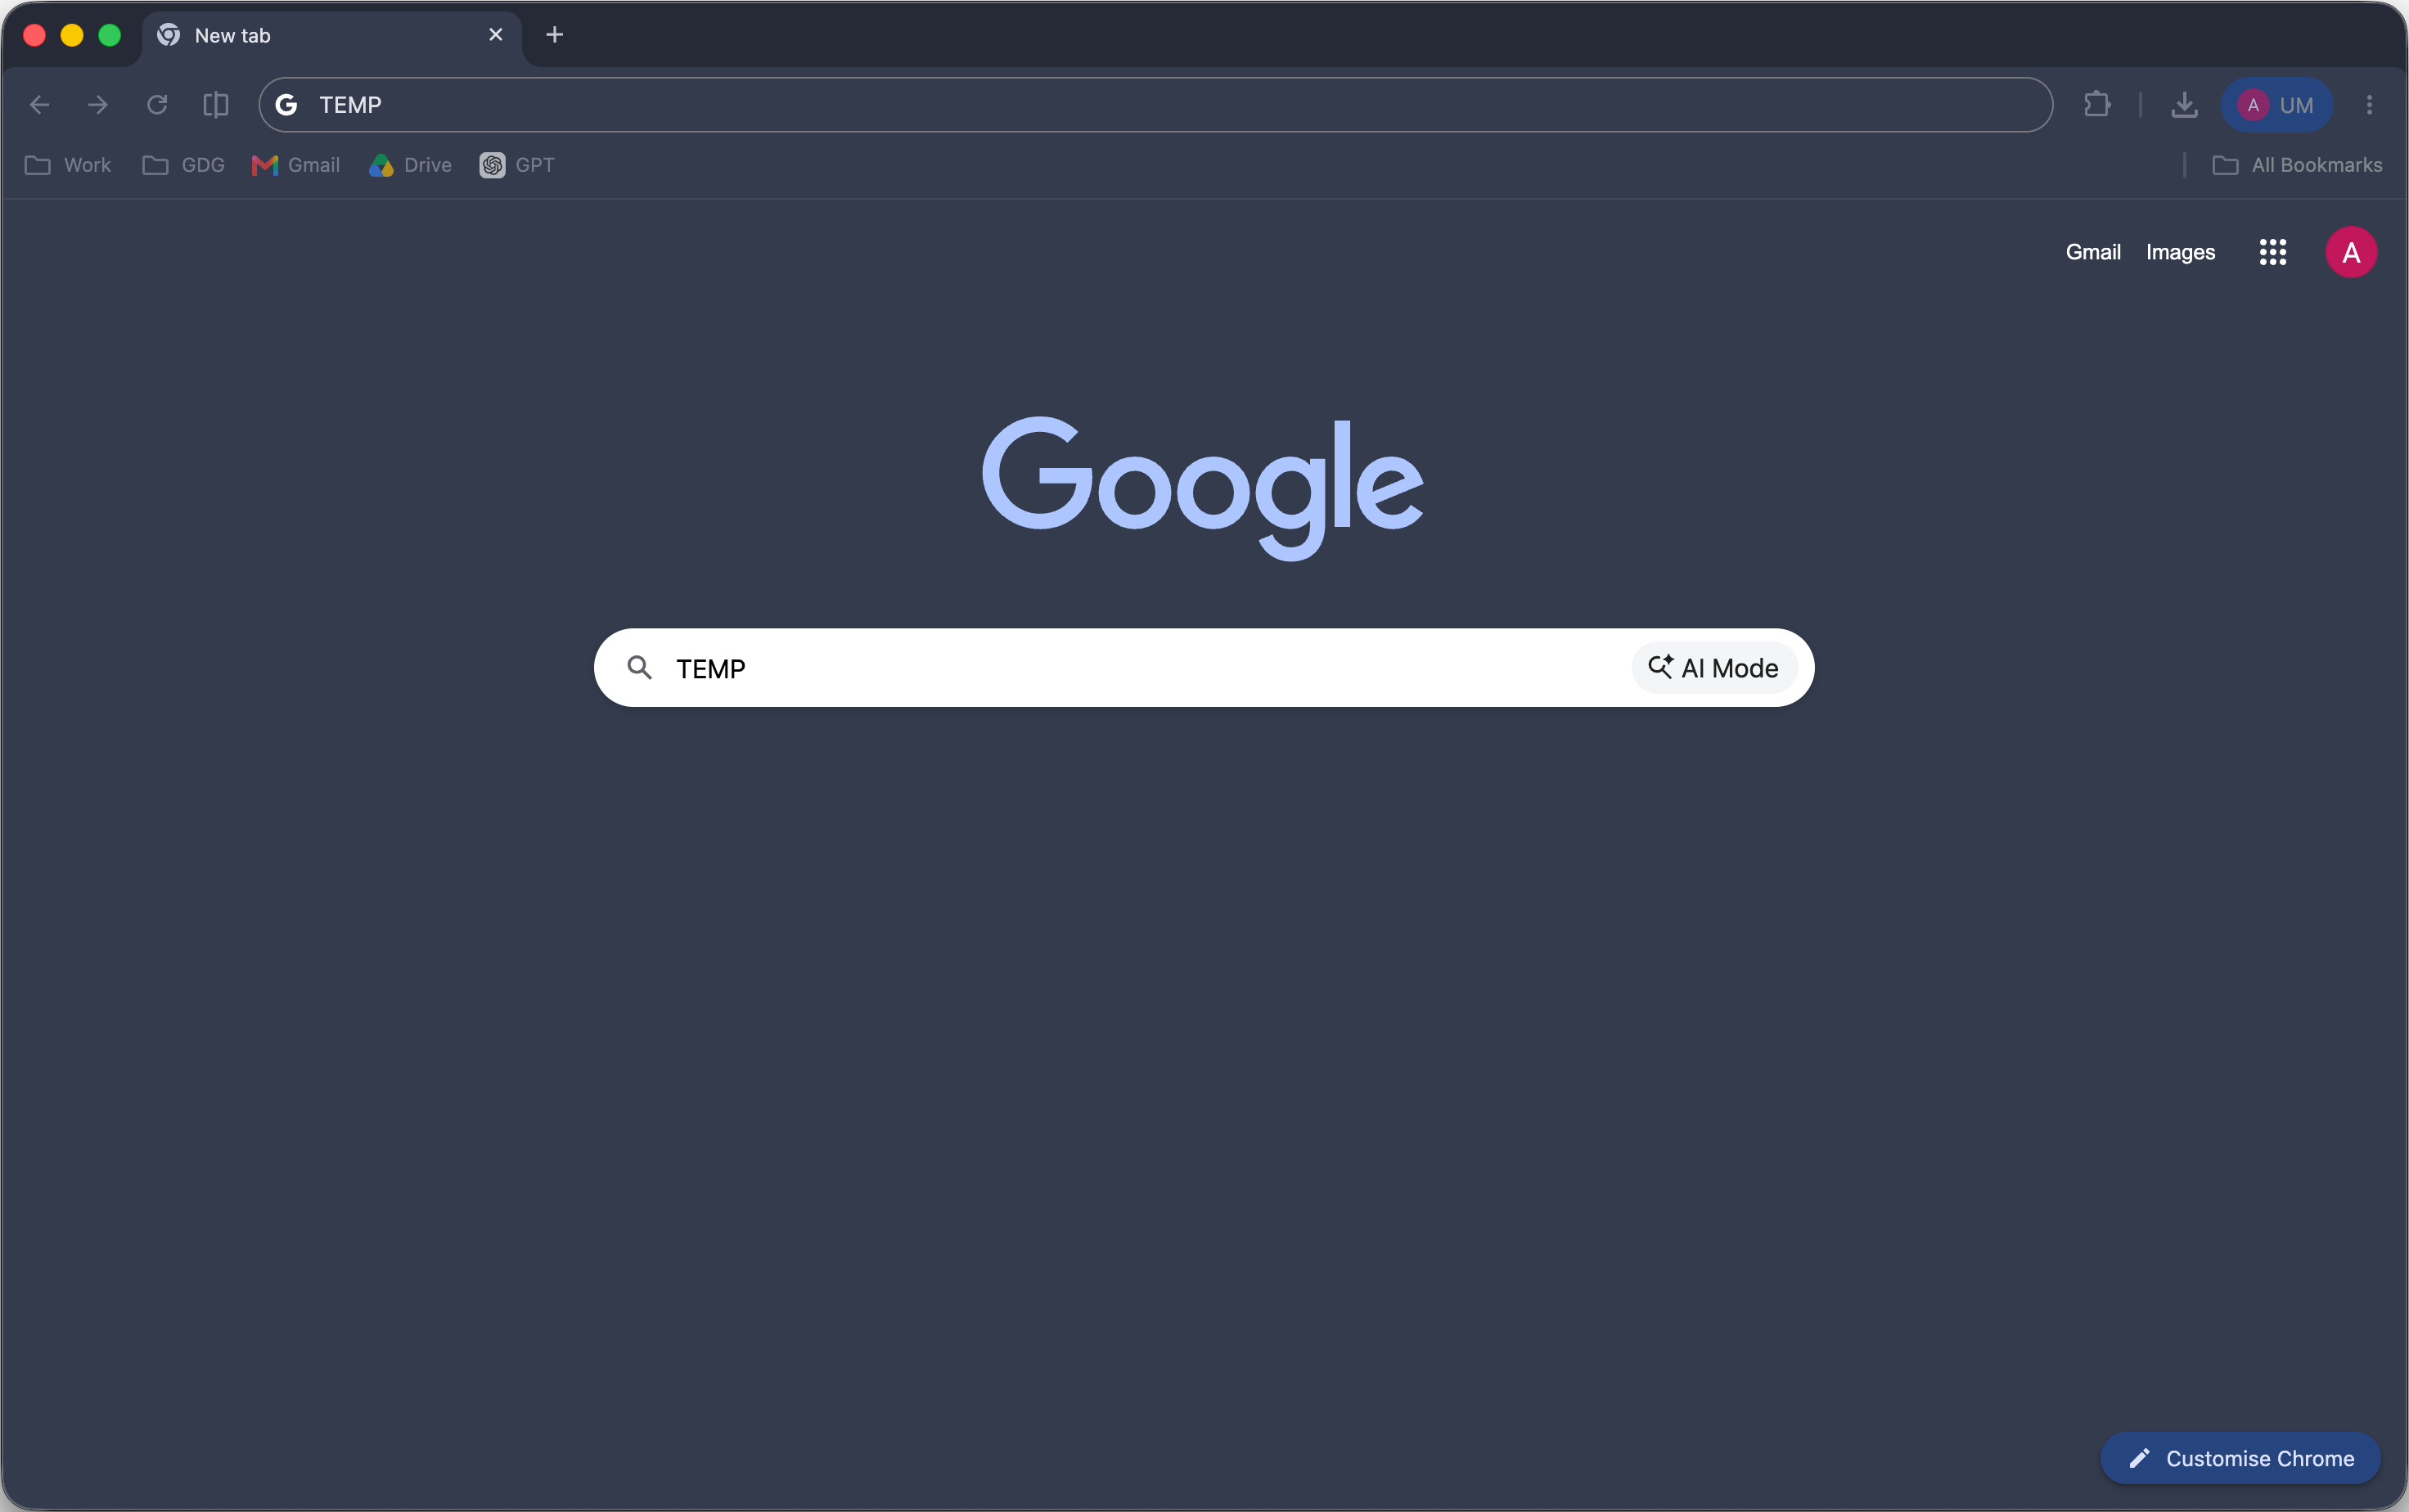
\includegraphics[width=\textwidth]{figures/PromptDetect-UI.png}
    \caption{\gls{UI} for exploratory prompt development, supporting free-text prompt entry, model selection, and visual inspection of predicted boxes and masks across the prompt-based models.}
    \label{fig:promptdetect-ui}
\end{figure}

\newpage
\noindent Within the \gls{MDWD}, the prompt inventory was structured to evaluate both category-specific and broader waste localisation, as summarised in Table~\ref{tab:primary-mdwd-prompts}. Four class-targeted prompts represent the principal colour-coded collection streams using terminology grou\-nded in their visible presentation, with bag colour retained because it provides an operational visual distinction between waste streams. The heterogeneous \textit{Other Waste} residual class was not assigned a dedicated class-targeted prompt because it does not represent a single visually or semantically coherent category. Two broader prompts instead map to the complete five-class \gls{MDWD} taxonomy, including \textit{Other Waste}, thereby extending the evaluation from individual waste streams to broader semantic localisation.

\begin{table}[H]
\centering
\small
\caption{\gls{MDWD} prompt inventory and corresponding positive \gls{GT} mappings.}
\label{tab:primary-mdwd-prompts}
\renewcommand{\arraystretch}{1.35}
\begin{tabularx}{\textwidth}{
    @{}
    >{\raggedright\arraybackslash}p{4.2cm}
    >{\raggedleft\arraybackslash}X
    @{}
}
\toprule
\textbf{Positive \gls{GT} class(es)} & \textbf{Prompt} \\
\midrule
\multicolumn{2}{@{}l}{\textbf{\textsc{Class-targeted prompts}}} \\
\cmidrule(lr){1-2}
Mixed Waste & \texttt{"Black garbage bag"} \\
Recyclable Material & \texttt{"Grey recycling bag"} \\
Organic Waste & \texttt{"White organic-waste bag"} \\
Orange \gls{CMD} & \texttt{"Orange garbage bag"} \\
\addlinespace[0.7em]
\multicolumn{2}{@{}l}{\textbf{\textsc{Broad prompts}}} \\
\cmidrule(lr){1-2}
All \gls{MDWD} classes & \texttt{"Domestic waste"} \\
All \gls{MDWD} classes & \texttt{"Garbage"} \\
\bottomrule
\end{tabularx}
\end{table}

\noindent The \gls{MTSD} required a broader prompt inventory because several categories admit multiple plausible natural-language descriptions. The inventory therefore distinguishes class-targeted, synonym-comparison and broad prompts, as shown in Table~\ref{tab:primary-mtsd-prompts}. Seven class-targeted prompts provide single-category localisation tasks using direct descriptions of the corresponding \gls{GT} classes. As with \emph{Other Waste} in the \gls{MDWD}, no class-targeted prompts were defined for \emph{Auxiliary Sign} or \emph{Other-Unknown}, since neither corresponds to a visually coherent concept describable by a natural-language query, though both remain eligible under the broad prompts. Four synonym-comparison prompts form two pairs that evaluate alternative terminology against the same target class. These are treated as terminology comparisons rather than controlled paraphrases because the expressions may differ in conventional meaning. The two broad prompts instead expand the semantic scope. \emph{Traffic sign} maps to the ten sign-related categories while excluding \textit{Blind-Spot Mirror (Convex Mirror)}, whereas \emph{roadside traffic-control object} encompasses the complete eleven-class \gls{MTSD} taxonomy.

\begin{longtable}{
    @{}
    >{\raggedright\arraybackslash}p{0.60\textwidth}
    >{\raggedleft\arraybackslash}p{0.34\textwidth}
    @{}
}
\caption{\gls{MTSD} prompt inventory and corresponding positive \gls{GT} mappings.}
\label{tab:primary-mtsd-prompts}\\
\toprule
\textbf{Positive \gls{GT} class(es)} & \textbf{Prompt} \\
\midrule
\endfirsthead
\toprule
\textbf{Positive \gls{GT} class(es)} & \textbf{Prompt} \\
\midrule
\endhead

\multicolumn{2}{@{}l}{\textbf{\textsc{Class-targeted prompts}}} \\
\cmidrule(lr){1-2}
Pedestrian Crossing & \texttt{"Pedestrian crossing sign"} \\
Stop Sign & \texttt{"Stop sign"} \\
Roundabout Ahead & \texttt{"Roundabout ahead sign"} \\
Blind-Spot Mirror (Convex Mirror) & \texttt{"Blind-spot convex mirror"} \\
Street Sign & \texttt{"Street sign"} \\
Directional Sign & \texttt{"Directional sign"} \\
Back-Unknown & \texttt{"Back of a traffic sign"} \\
\addlinespace[0.7em]

\multicolumn{2}{@{}l}{\textbf{\textsc{Synonym-comparison prompts}}} \\
\cmidrule(lr){1-2}
No Entry (One Way) & \texttt{"No entry sign"} \\
No Entry (One Way) & \texttt{"One way sign"} \\
No Through Road (T-Junction) & \texttt{"No through road sign"} \\
No Through Road (T-Junction) & \texttt{"T-junction sign"} \\
\addlinespace[0.7em]

\multicolumn{2}{@{}l}{\textbf{\textsc{Broad prompts}}} \\
\cmidrule(lr){1-2}
All \gls{MTSD} classes, excluding Blind-Spot Mirror (Convex Mirror)
& \texttt{"Traffic sign"} \\
All \gls{MTSD} classes, including Blind-Spot Mirror (Convex Mirror)
& \texttt{"Roadside traffic-control object"} \\
\bottomrule
\end{longtable}

\noindent The principal cross-model comparison is calculated as a prompt-level macro-average across class-targeted and synonym-comparison prompts. Each query maps to a single \gls{GT} category and therefore represents a comparable category-level localisation task. Synonym variants are retained as separate observations to assess whether alternative terminology affects localisation performance for the same target class. Broad prompts are evaluated separately because they span multiple \gls{GT} categories, increasing the number and diversity of eligible targets. Including them in the aggregate would therefore confound prompt specificity with model performance.

\newpage 
\subsection{Prediction Normalisation and Post-Processing}
\label{sec:prediction-normalisation}
For each prompt condition, the same semantic query was presented to all models, with only the formatting required by each architecture differing. \gls{SAM}~3 and 3.1 accept the query directly and natively return bounding boxes, confidence scores and segmentation masks. The masks were retained for inspection in the interactive \gls{UI} but excluded from quantitative evaluation since neither dataset provides instance-mask \gls{GT}. Cosmos Reason2 and LocateAnything instead require textual localisation outputs, with Cosmos Reason2 instructed to return a \gls{JSON} list of \texttt{bbox\_2d} coordinates and labels and LocateAnything returning four-coordinate \texttt{<box>} tokens through its native multi-instance grounding formulation. Decoding was deterministic, with generation length bounded by the permitted prediction count, and both parsers discarded malformed box records while tolerating surrounding generated text. The resulting predictions from all models were then converted to source-image pixel coordinates in \((x_0, y_0, x_1, \\y_1)\) format, with the \(0\)--\(1000\) coordinates produced by Cosmos Reason2 and LocateAnything rescaled accordingly, before being clipped to valid image bounds and evaluated in the same coordinate system.

\begin{figure}[H]
\centering
    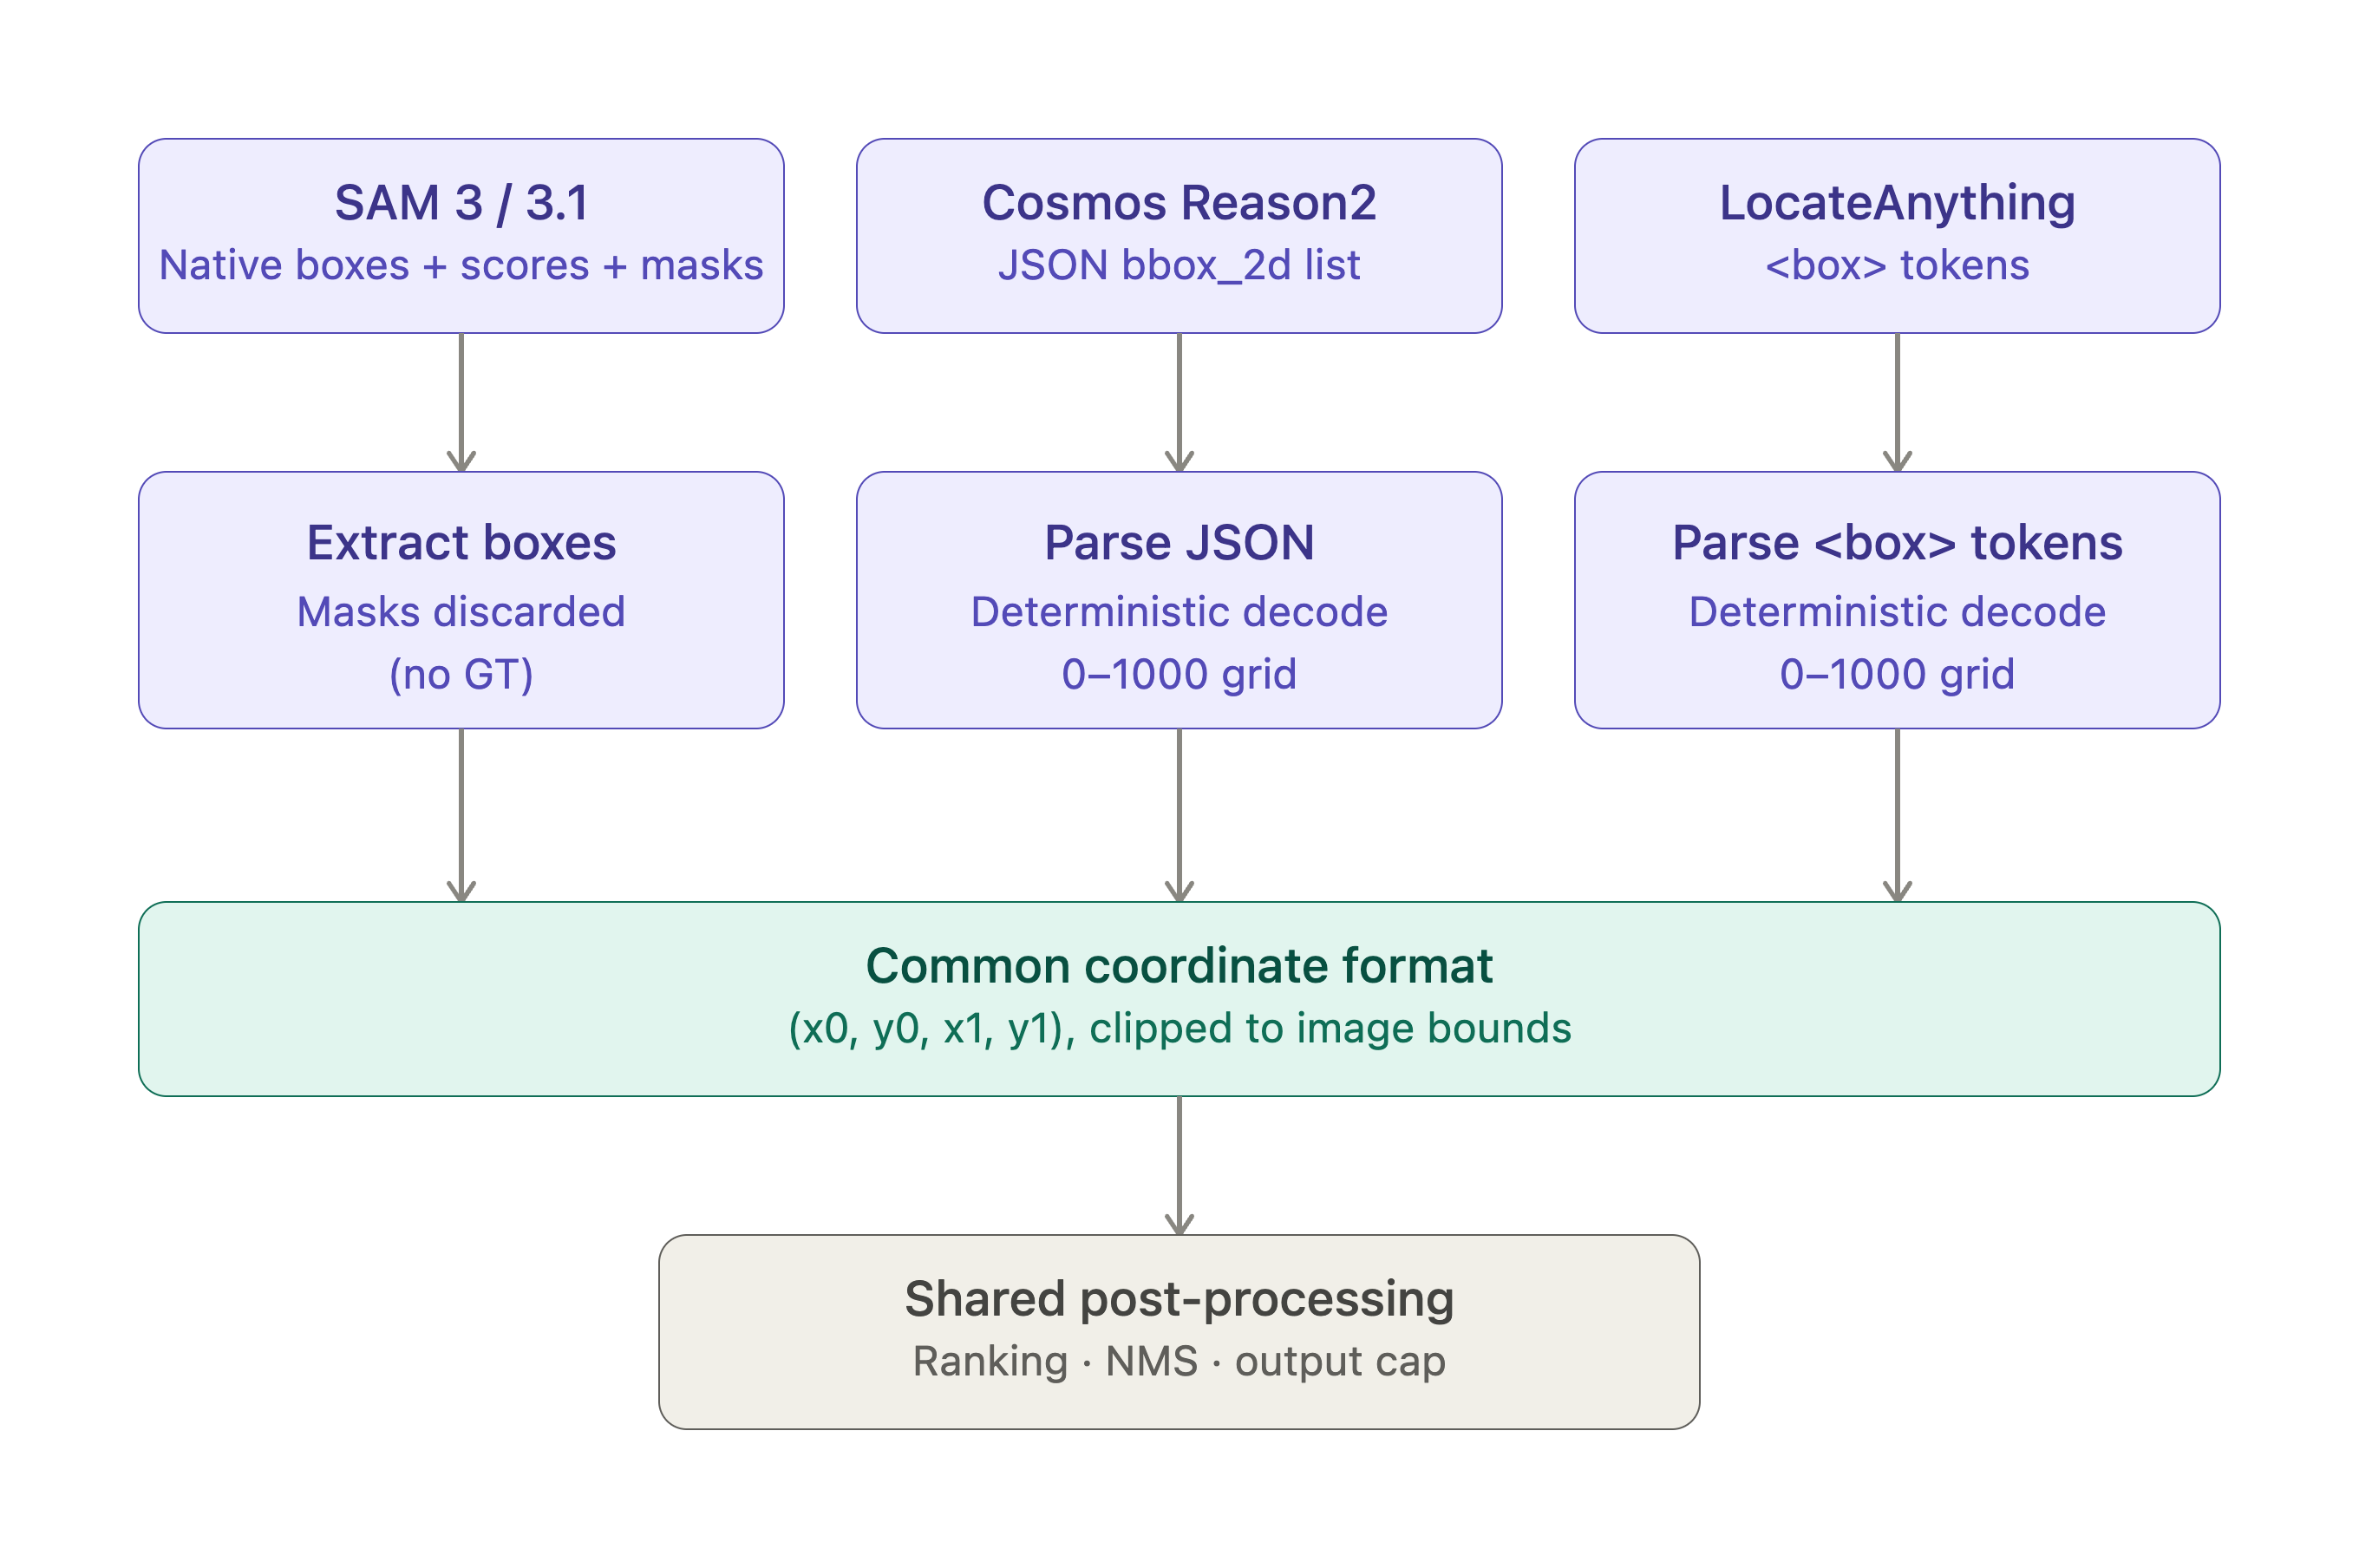
\includegraphics[width=\textwidth]{figures/prediction-normalisation-pipeline.png}
    \caption{Normalisation of model-specific outputs to a common coordinate format.}
    \label{fig:prediction-normalisation-pipeline}
\end{figure}

\newpage
\noindent Each inference call constituted a single semantic query, so \gls{NMS} was applied class-agnost\-ically, ranking predictions by confidence where available prior to suppression and output limiting. As LocateAnything and Cosmos Reason2 provide no per-box confidence, their predictions received a uniform score of \(1.0\), with stable sorting preserving generation order, leaving confidence-ranked \gls{AP} directly interpretable only for \gls{SAM}~3 and 3.1 and cross-model comparison reliant instead on the fixed-operating-point measures defined in Chapter~\ref{ch:evaluation}.

\subsection{Inference Execution and Runtime Measurement}
\label{sec:inference-execution}
Inference was process-isolated to bound memory use and provide a reliable recovery boundary between runs. Each \gls{SAM} model--prompt combination was executed in a fresh worker process over the complete evaluated image set. LocateAnything-3B used fresh workers for successive chunks of up to 64 images, whereas Cosmos Reason2 used smaller eight-image chunks to constrain \gls{RAM} and \gls{VRAM} growth. Each worker loaded the required model, persisted its predictions and completion status, and then terminated, making process exit the principal memory-cleanup boundary.

Model-specific input resizing was applied only where required by the inference architecture. LocateAnything images with a longest side exceeding 1536 pixels were downscaled before inference. Cosmos Reason2 used checkpoint-specific maximum sides of 2560 pixels for the 2B model and 1536 pixels for the 8B model. Source images remained unchanged, with localisation outputs mapped to their original image dimensions for evaluation.

Completed chunks and model--prompt combinations were reused only when their stored experimental fingerprint matched the active configuration, including the protocol and dataset hashes, model, prompt text, target classes, split, detection limits and evaluation thresholds. Incompatible stored results were rejected, allowing interrupted evaluations to resume without mixing predictions generated under different experimental settings.

Reported localisation latency was measured per image around the complete prediction call after source-image loading. Model initialisation, worker creation, image loading and result persistence were therefore excluded. The measurement included model-specific preprocessing, prompt preparation, inference or generation, output parsing, coordinate conversion, prediction filtering and \gls{NMS}. Reported latency consequently represents end-to-end prediction-pipeline latency rather than neural-network forward-pass time alone.

\newpage
\subsection{Taxonomy-Aware Ground-Truth Mapping}
\label{sec:prompt-matching}

The semantic mappings introduced in Subsection~\ref{sec:prompt-inventory} were formalised so that each query was evaluated only against the classes it was intended to retrieve. For prompt \(q\), let \(\mathcal{C}_q\) denote its predefined set of eligible classes. For image \(i\), the corresponding target \gls{GT} set was defined as:

\begin{equation}
G_i^{(q)} =
\left\{
g \in G_i :
\mathrm{class}(g) \in \mathcal{C}_q
\right\}.
\end{equation}

\noindent Annotations outside \(\mathcal{C}_q\) remained present as non-target objects, while images containing no eligible targets were retained so that erroneous predictions in target-absent scenes remained measurable. Unmatched predictions overlapping a non-target annotated object at \(\mathrm{IoU} \geq 0.50\) remained \glspl{FP}, but were recorded separately by non-target class to distinguish semantic confusion from predictions occurring on background or unannotated regions. 

\subsection{Controlled Prompt-Sensitivity Experiment}
\label{sec:prompt-sensitivity}
A controlled experiment examined the sensitivity of prompt-based localisation to changes in linguistic formulation. Unlike the broader and synonym-comparison queries used in the primary evaluation, all prompts within a sensitivity family shared the same target \gls{GT} set, with only their wording varied. Differences in localisation performance within a family could therefore be attributed more directly to prompt formulation rather than to changes in target-class scope.

Nine target families were evaluated: four from the \gls{MDWD}, corresponding to \emph{Mixed Waste}, \emph{Recyclable Material}, \emph{Organic Waste} and \emph{Orange \gls{CMD}}, and five from the \gls{MTSD}, corresponding to \emph{Pedestrian Crossing}, \emph{Stop Sign}, \emph{Roundabout Ahead}, \emph{No Entry (One Way)} and \emph{Blind-Spot Mirror(Convex Mirror)}. Each family contained four formulations designed to vary the linguistic expression of the query while preserving the same underlying target concept. The formulation types and their intended distinction are summarised in Table~\ref{tab:prompt-sensitivity-types} using \emph{Mixed Waste} as an illustrative example.

Within each family, all four formulations shared an identical target-class set and were evaluated on the same canonical test split. The protocol additionally verified identical positive-image, negative-image and target-box counts across variants, ensuring that observed differences reflected changes in prompt wording rather than changes in evaluation scope. The complete prompt inventory is provided in Appendix~\ref{app:prompt-sensitivity-prompts}.

The heterogeneous \emph{Other Waste} category was excluded because it represents a residual class for which a coherent set of semantically equivalent prompts could not be defined. Similarly, \emph{one way sign} was retained only within the synonym-comparison analysis because it is not a controlled paraphrase of \emph{no entry sign}.

\begin{table}[H]
\centering
\small
\caption{Prompt formulation types used in the prompt-sensitivity experiment.}
\label{tab:prompt-sensitivity-types}
\renewcommand{\arraystretch}{1.25}
\begin{tabularx}{\textwidth}{
    @{}
    >{\raggedright\arraybackslash}p{3.2cm}
    >{\raggedright\arraybackslash}X
    >{\raggedright\arraybackslash}p{5.0cm}
    @{}
}
\toprule
\textbf{Variant} & \textbf{Purpose} & \textbf{Example: Mixed Waste} \\
\midrule

Canonical
& Concise noun phrase used in the primary prompt inventory.
& \texttt{"Black garbage bag"} \\

Lexical paraphrase
& Rephrases the concept using alternative but semantically related terminology.
& \texttt{"Black refuse bag"} \\

Descriptive paraphrase
& Expresses the target through a fuller visual or semantic description.
& \texttt{"Black bag containing mixed household waste"} \\

Instruction
& Reformulates the same target as an explicit localisation request.
& \texttt{"Find all black mixed-waste bags"} \\

\bottomrule
\end{tabularx}
\end{table}

\noindent For each model and target family, precision, recall, \(F_1\) and mean matched-box \gls{IoU} were calculated independently for all four formulations. Prompt sensitivity was characterised using the mean, population standard deviation, minimum, maximum and range of each metric across the four variants. Absolute \(F_1\) variation was defined as:

\begin{equation}
\Delta F_1 =
\max(F_1) - \min(F_1),
\end{equation}

\noindent with relative degradation defined as:

\begin{equation}
\Delta F_{1,\mathrm{rel}} =
\frac{\max(F_1)-\min(F_1)}
{\max(F_1)}.
\end{equation}

\noindent Where all four formulations produced \(F_1=0\), relative degradation was set to zero for numerical completeness and interpreted as consistent failure rather than prompt robustness. The analysis additionally retained the best- and worst-performing formulations, the canonical and instruction-style \(F_1\) scores, and each non-canonical variant's deviation from the canonical \(F_1\).

Prompt stability was assessed independently of \gls{GT} through all six pairwise comparisons among the four prediction sets within each family. Predicted boxes were greedily matched at \(\mathrm{IoU}=0.50\). For two prediction sets containing \(N_A\) and \(N_B\) boxes, with \(M\) matched pairs, pairwise agreement was defined as:

\begin{equation}
F_{1,\mathrm{pair}} =
\frac{2M}{N_A+N_B},
\qquad
J_{\mathrm{pair}} =
\frac{M}{N_A+N_B-M}.
\end{equation}

\noindent Mean \gls{IoU} across matched prediction pairs and unmatched-box counts were also retained. Two empty prediction sets were treated as fully consistent, with \(F_{1,\mathrm{pair}}=J_{\mathrm{pair}}=1\). These consistency measures quantify stability in model output rather than localisation correctness and are therefore interpreted alongside the corresponding \gls{GT}-based performance measures.

\section{Multi-Attribute Traffic-Sign Classification}
\label{sec:attr-cls}
The third experimental track evaluates the transferability of pretrained visual representations to the four object-level attributes defined for the \gls{MTSD}, formulated as a multi-task classification problem in which each \gls{GT} traffic-sign crop is encoded once by a shared visual backbone and passed to four independent classification heads. Each head performs single-label classification within its respective attribute space, avoiding the sparse combinatorial label space that would result from treating every attribute combination as a separate class, while allowing the shared representation to support related visual cues across tasks.

Attribute classification uses the final \gls{QA}-approved \gls{MTSD} annotations, partitioned and cropped as described in Subsections~\ref{sec:md-partitioning} and~\ref{sec:md-augmentation-attribute}. Instances whose original \gls{GT} bounding box measured fewer than 20 pixels along either dimension were excluded because the available visual information was considered insufficient for reliable attribute recognition. This removed 1,256 of the 20,509 annotated instances, producing a fixed experiment-ready manifest of 19,253 crops: 15,465 for training, 1,898 for validation and 1,890 for testing. All retained crops contain valid supervision for the four modelled attributes, and the same manifest was used throughout the representation and adaptation experiments.

\subsection{Visual Representations and Experimental Design}
\label{sec:attribute-backbones}
Four pretrained visual-representation families were selected to span different architectural and pre-training paradigms. \gls{DINO}v3, \gls{VJEPA}~2.1 and LingBot-Vision use \gls{VIT}-based architectures, whereas ConvNeXt provides a convolutional counterpart pretrained through supervised ImageNet-1K classification. Base (-B) and Large (-L) configurations were evaluated for each family, allowing model capacity to be considered alongside representation type and adaptation strategy, as summarised in Table~\ref{tab:attribute-backbone-matrix}.

The experimental matrix comprises 18 principal configurations, comprising frozen linear probing and \gls{LoRA} adaptation for both capacities of all four families, together with full \gls{FT} for ConvNeXt-B and ConvNeXt-L. Full \gls{FT} was not evaluated for the \gls{VIT}-based families, as the memory requirements of end-to-end adaptation exceeded the practical limits of the available training hardware. The experiment therefore compares feasible representation--adaptation combinations rather than a fully crossed architecture-by-adaptation factorial design.

\begin{table}[H]
\centering
\caption{Representation families and adaptation strategies for multi-attribute traffic-sign classification.}
\label{tab:attribute-backbone-matrix}
\renewcommand{\arraystretch}{1.3}
\small
\begin{tabularx}{\textwidth}{
    @{}
    >{\raggedright\arraybackslash}p{2.6cm}
    >{\centering\arraybackslash}p{2.1cm}
    >{\centering\arraybackslash}p{2.1cm}
    >{\centering\arraybackslash}p{1.5cm}
    >{\centering\arraybackslash}p{1.5cm}
    >{\centering\arraybackslash}p{1.8cm}
    >{\centering\arraybackslash}p{1.8cm}
    @{}
}
\toprule
& \multicolumn{2}{c}{\textbf{Capacity}} & \multicolumn{3}{c}{\textbf{Adaptation Strategy}} & \\
\cmidrule(lr){2-3}\cmidrule(lr){4-6}
\textbf{Family} & \textbf{Base} & \textbf{Large} & \textbf{Frozen} & \textbf{\gls{LoRA}} & \textbf{Full \gls{FT}} & \textbf{Input Size} \\
\midrule
\gls{DINO}v3
& \gls{VIT}-B/16 & \gls{VIT}-L/16
& \checkmark & \checkmark & --
& \(224\times224\) \\
\gls{VJEPA}~2.1
& \gls{VIT}-B/16 & \gls{VIT}-L/16
& \checkmark & \checkmark & --
& \(384\times384\) \\
ConvNeXt
& Base & Large
& \checkmark & \checkmark & \checkmark
& \(224\times224\) \\
LingBot-Vision
& \gls{VIT}-B/16 & \gls{VIT}-L/16
& \checkmark & \checkmark & --
& \(224\times224\) \\
\bottomrule
\end{tabularx}
\end{table}

\subsubsection{Model Initialisation and Feature Extraction}
\label{sec:attrcls-initialisation}
All backbones were initialised from publicly released pretrained weights rather than trained from random initialisation. \gls{DINO}v3\footnote{\url{https://github.com/facebookresearch/dinov3}} was loaded through Hugging Face \texttt{transfo\-rmers} using the corresponding \texttt{facebook/dinov3-*-pretrain-lvd1689m} checkpoints. Its pooled CLS representation---\texttt{pooler\_output} where provided by the implementation,
otherwise the first output token---was used as the crop-level feature vector. \gls{VJEPA}~2.1\footnote{\url{https://github.com/facebookresearch/vjepa2}} was loaded through Meta's official \texttt{torch.hub} entry points and released \gls{VJEPA}~2.1 checkpoints, with fallback to \gls{VJEPA}~2.0 explicitly disabled; its encoder output tokens were mean-pooled to obtain a single crop-level representation. LingBot-Vision\footnote{\url{https://github.com/robbyant/lingbot-vision}} was loaded through the official \texttt{lingbot\_vision} interface, with normalised patch-token representations mean-pooled.  ConvNeXt-B and ConvNeXt-L\footnote{\url{https://pytorch.org/vision/stable/models/convnext.html}} were initialised directly thro\-ugh torchvision's corresponding model implementations with \texttt{IMAGENET1K\_V1} pretrained weights, applying global average pooling to the final spatial feature map.

As \gls{VJEPA}~2.1 is pretrained for video input, each static \gls{MTSD} crop was repeated along the temporal dimension to form a two-frame pseudo-clip matching the model's tubelet size. This satisfies the expected temporal input structure without introducing synthetic motion or additional visual information, allowing the video-pretrained representation to be evaluated within the same static-image classification framework as the image-based backbones. In every case, the resulting crop-level representation was supplied to the four attribute-specific classification heads, with model identifiers, loader backends, feature dimensions and parameter counts retained throughout for reproducibility.

\subsection{Adaptation Strategies}
\label{sec:attribute-adaptation}
Three adaptation regimes were implemented to vary the extent to which the pretrained representation was modified during transfer. In the frozen setting, all backbone parameters remained fixed and the backbone was retained in evaluation mode throughout training, such that optimisation was restricted to the four newly initialised classification heads. This provides a direct assessment of the separability of the target attributes using the pretrained representation without altering its underlying feature space.

Under \gls{LoRA} adaptation, the original backbone weights likewise remained frozen, while low-rank adapters and the classification heads were jointly optimised. All \gls{LoRA} configurations used rank \(r=8\), scaling factor \(\alpha=16\), dropout of 0.05 and \texttt{bias="none"}, ensuring that no pretrained backbone bias terms were updated. Adapter placement followed the internal structure of each backbone: \gls{DINO}v3 targeted the separate attention \texttt{q\_proj} and \texttt{v\_proj} transformations, whereas \gls{VJEPA}~2.1 and LingBot-Vision targeted their fused \texttt{qkv} projections. For ConvNeXt, adapters were inserted into the two pointwise linear layers of each block (\texttt{block.3} and \texttt{block.5} in the torchvision implementation), with target specifications applied to all matching modules in the loaded backbone and verified before optimisation to confirm correct insertion.

Full \gls{FT} was applied only to ConvNeXt-B and -L, for which both the pretrained backbone and the four classification heads were updated during optimisation. For every configuration, the parameter audit reported total and trainable parameters, while further separating trainable head and adapter parameters and recording the trainable proportion of the complete model. This enables the extent of task-specific adaptation to be considered alongside predictive performance.

\begin{figure}[H]
\centering
    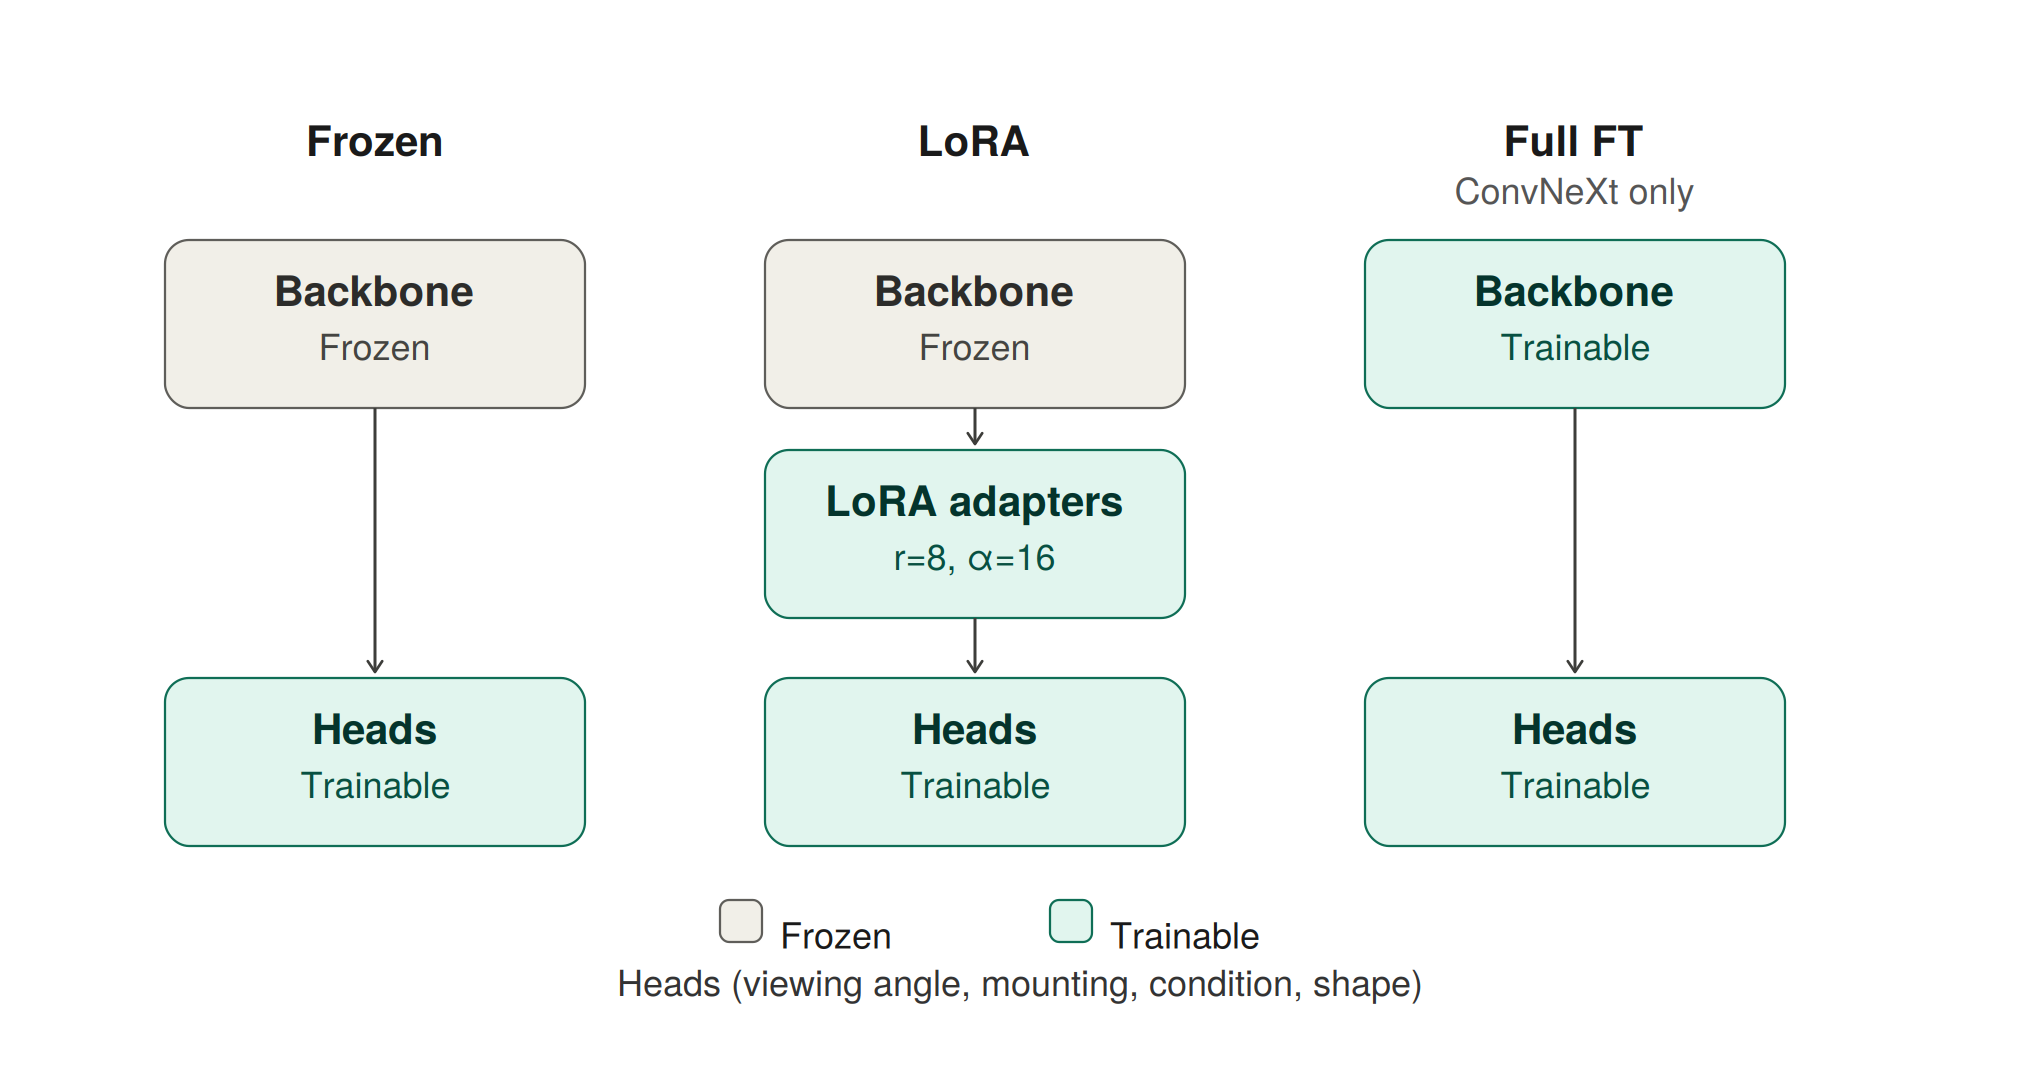
\includegraphics[width=0.95\textwidth]{figures/adaptation-strategies.png}
    \caption{Comparison of the three adaptation strategies evaluated for multi-attribute traffic-sign classification.}
    \label{fig:adaptation-strategies}
\end{figure}

\newpage
\subsection{Shared Multi-Head Architecture and Optimisation}
\label{sec:attribute-training}
Irrespective of backbone or adaptation strategy, the same downstream classification formulation was retained. For an input crop \(x\), the selected backbone \(f_{\theta}\) produces a pooled visual representation: 

\begin{equation}
\mathbf{z}=f_{\theta}(x),
\end{equation}

\noindent each attribute \(a\) is then predicted independently through a linear classification head,

\begin{equation}
\mathbf{o}_{a}
=
\mathbf{W}_{a}\mathbf{z}
+
\mathbf{b}_{a},
\end{equation}

\noindent where \(\mathbf{o}_{a}\) contains the logits for the classes belonging to attribute \(a\). The four heads share the backbone representation but contain no parameters in common with one another. This avoids four independent feature-extraction passes while retaining attribute-specific output spaces and loss functions. Class imbalance was addressed using weighted cross-entropy independently for each head. For class \(c\) within attribute \(a\), the class weight was calculated from the training partition as:

\begin{equation}
\label{eq:attr-class-weight}
w_{a,c}
=
\frac{N_a}{C_a n_{a,c}},
\end{equation}

\noindent where \(N_a\) denotes the number of training instances for attribute \(a\), \(C_a\) its number of classes and \(n_{a,c}\) the number of training instances belonging to class \(c\). This inverse-frequency formulation increases the contribution of less frequently represented classes while maintaining a frequency-weighted mean class weight of one within each task. For an instance with reference class \(y_a\), the loss for attribute \(a\) is:

\begin{equation}
\mathcal{L}_{a}
=
-w_{a,y_a}
\log p_{a,y_a},
\end{equation}

\noindent where \(p_{a,y_a}\) denotes the predicted probability assigned to the reference class. The overall optimisation objective is the unweighted sum of the four attribute losses, each term corresponding to its respective sign attribute:

\begin{equation}
\mathcal{L}_{\mathrm{joint}}
=
\mathcal{L}_{\mathrm{angle}}
+
\mathcal{L}_{\mathrm{mounting}}
+
\mathcal{L}_{\mathrm{condition}}
+
\mathcal{L}_{\mathrm{shape}}.
\end{equation}

\noindent Equal task weighting was retained so that no attribute received greater importance a priori, with class imbalance addressed independently within each head and no label smoothing applied. Per-head masking of missing labels was implemented as a defensive measure but never exercised, since the final manifest contains valid supervision for all four attributes.

\subsection{Training Procedure}
\label{sec:trainingprod}
A common optimisation protocol was applied across the 18 principal configurations to minimise procedural variation between representation families, model capacities and adaptation strategies. Shared settings and model- or adaptation-specific exceptions are summarised in Table~\ref{tab:attribute-training-config}.

\begin{table}[H]
\centering
\caption{Training configuration used for the multi-attribute classification experiments. Values are shared unless a model- or adaptation-specific exception is indicated.}
\label{tab:attribute-training-config}
\renewcommand{\arraystretch}{1.18}
\small
\begin{tabularx}{\textwidth}{
    @{}
    >{\raggedright\arraybackslash}p{5.0cm}
    >{\raggedleft\arraybackslash}X
    @{}
}
\toprule
\textbf{Setting} & \textbf{Configuration} \\
\midrule

Random seed
& 42 \\

Maximum epochs
& 150 \\

Optimiser
& AdamW \\

Weight decay
& 0.05 \\

Learning-rate schedule
& 5-epoch linear warm-up followed by cosine decay to zero \\

\addlinespace[0.35em]

Head learning rate
& \(1\times10^{-3}\) (frozen/\gls{LoRA}); \(4\times10^{-4}\) (full \gls{FT}) \\

\gls{LoRA} learning rate
& \(2\times10^{-4}\) \\

Fine-tuned backbone learning rate
& \(5\times10^{-5}\) \\

\addlinespace[0.35em]

DataLoader workers
& 4 \\

Effective batch size
& 32 \\

Physical batch size and accumulation
& \(32\times1\), or \(16\times2\) for variants requiring reduced physical batches \\

Gradient clipping
& Global norm \(=1.0\) \\

Mixed precision
& \gls{BF16} autocasting where supported \\

\addlinespace[0.35em]

Loss
& Class-weighted cross-entropy \\

Class weighting
& Per-attribute inverse-frequency weights calculated from the training split (Eq.~\ref{eq:attr-class-weight}) \\

Task weighting
& Equal weighting across all four heads \\

Missing labels
& Masked independently for the affected attribute head \\

\addlinespace[0.35em]

Early-stopping patience
& 10 epochs \\

Minimum improvement
& \(0.001\) validation mean macro-\(F_1\) \\

\bottomrule
\end{tabularx}
\end{table}

\newpage
\noindent Separate learning rates were assigned to the classification heads, \gls{LoRA} adapters and fully \gls{FT} backbone parameters to reflect their different initialisation states. Newly initialised heads therefore received larger updates, while pretrained backbone parameters were adapted more conservatively. Where the standard physical batch size exceeded available \gls{GPU} memory, gradient accumulation preserved an effective batch size of 32. Automatic batch-size reduction was disabled so that memory constraints could not silently alter the experimental configuration.

Checkpoint selection used validation mean macro-\(F_1\), calculated as the unweight\-ed mean of the four attribute-level macro-\(F_1\) scores. Early stopping was triggered after 10 consecutive epochs without an improvement exceeding \(0.001\), whereas checkpoint selection remained independent of this threshold, with any strict improvement updating the best checkpoint. Following training, only the checkpoint with the highest validation mean macro-\(F_1\) was evaluated on the held-out test partition.

These experiments were run on the same workstation used for the supervised \glspl{OD} and prompt-based localisation experiments. Python~3.11.15, PyTorch~2.11.0, \gls{CUDA} 12.8 and \gls{CUDNN}~9.19 were used, together with torchvision~0.26.0, Transformers~5.12.1, \gls{PEFT}~0.19.1, timm~1.0.27 and lingbot-vision~0.1.0. Python, NumPy and PyTorch \gls{CPU} and \gls{CUDA} random-number generators were seeded at 42. Configuration snapshots, dataset manifests, included group and split counts, class weights, checkpoints, evaluation outputs and the corresponding Git commit were retained for each run. Exact bitwise replication is not claimed, as \gls{CUDNN} autotuning, parallel data loading and mixed-precision operations were not constrained to fully deterministic execution.

\noindent\rule{\linewidth}{0.3pt}
% Draft grounded in repository exports; methodology.tex is authoritative.
% Audit trail: evaluation_sources.md in this directory. No figures generated.
\chapter{Evaluation \& Results}
\label{ch:evaluation}
This chapter evaluates the three experimental tracks defined in Chapter~\ref{ch:methodology}: supervised \gls{OD}, zero-shot prompt-based localisation, and multi-attribute traffic-sign classification. The analysis considers predictive performance alongside model capacity, sensitivity to the experimental configuration and computational requirements. Results are interpreted within the two Maltese street-level domains, with particular attention to small-object localisation, semantic ambiguity and the recognition of physical condition.

The chapter draws on the retained test summaries, prediction exports and evaluation records. Where these records differ from the protocol established in Chapter~\ref{ch:methodology}, the discrepancy is identified rather than treating the available measurement as an exact implementation of that protocol. Validation-only evaluations, earlier attribute experiments and prompt-localisation pilots are not substituted for final test results. All predictive measures in the tables are expressed as percentages unless otherwise stated; differences between them are expressed in percentage points.

\section{Evaluation Framework and Performance Measures}
\label{sec:ev-framework}
\subsection{Evaluation Protocol and Ground-Truth Matching}
\label{sec:ev-protocol}
The held-out localisation sets comprise 369 \gls{MDWD} images and 747 \gls{MTSD} images. Attribute classification instead uses the 1,890 eligible test crops inherited from the source-image partitions, following the minimum-size restriction in Section~\ref{sec:attr-cls}. The classification results therefore quantify characterisation of annotated objects with known bounding boxes, rather than the performance of a complete detection-and-characterisation pipeline.

For localisation, a prediction constitutes a \gls{TP} when it is assigned to an eligible \gls{GT} box at \(\mathrm{IoU}\geq0.50\), subject to one-to-one assignment. Unmatched predictions constitute \glspl{FP}, while unmatched eligible annotations constitute \glspl{FN}. Supervised evaluation additionally requires agreement with the annotated category. In prompt-based evaluation, eligibility is determined by the query-specific target-class mapping in Section~\ref{sec:prompt-matching}. Images containing no eligible targets remain in the evaluation, so a model cannot obtain high precision merely by being assessed on scenes known to contain the requested object.

The retained prompt evaluator processes predictions in descending score order and assigns each prediction to its highest-overlap target. A further prediction whose highest-overlap target has already been assigned is counted as a duplicate and a \gls{FP}; the implementation does not seek a second-best unassigned target in that case. This detail is relevant in crowded scenes and distinguishes the stored implementation from an optimal global assignment. Predictions from LocateAnything and Cosmos Reason2 have uniform scores, preserving generation order. The confidence threshold of 0.30, minimum box area of 100 pixels$^2$, \gls{NMS} threshold of 0.50 and dataset-specific output limits follow Table~\ref{tab:prompt-fixed-settings}.

Training and validation remain distinct from test evaluation. In particular, the attribute checkpoint is selected by validation mean macro-\(F_1\), and only the selected checkpoint is assessed on test crops. For \gls{MDWD}, the native summaries contain separate validation and test fields; only the explicitly identified test fields are used in the principal detector table. Their precision and recall retain the framework's native reporting convention, and the stored summary \(F_1\) is retained without treating it as a pooled object-level count statistic.

A further distinction is necessary for the unified \gls{MTSD} exports. Their precision, recall and standard \(F_1\) are calculated from pooled \gls{TP}, \gls{FP} and \gls{FN} counts using Equation~\ref{eq:ev-prf}, at the confidence value maximising \(F_1\) on the evaluated partition. The test tables report this ordinary harmonic-mean \(F_1\) without a separate starred notation. Because the operating threshold is selected on the same test partition, however, the reported value describes the best stored test-set precision--recall trade-off and is not an unbiased deployment estimate. Confidence-ranked \gls{AP} remains the principal measure for supervised configuration comparisons. The unified YOLO export retains predictions down to confidence 0.001, with \gls{NMS} at 0.70 and a maximum of 100 detections, so its prediction-generation settings also differ from the prompt pipeline.

\paragraph{MTSD taxonomy and implementation limitation.}
Methodology excludes \emph{Tourist Sign} from the experiment-ready localisation taxonomy and specifies that its boxes remain as ignore regions. The available unified exports evaluate 11 categories, containing 1,975 target boxes across the 747 test images. However, the retained supervised evaluator removes the excluded category's annotations and predictions by category identifier, without suppressing otherwise eligible predictions that overlap its boxes. The retained prompt matching code likewise contains no explicit Tourist Sign overlap-ignore operation. Moreover, some supervised run records explicitly retain the training taxonomy while excluding Tourist Sign only during evaluation. The stored measurements therefore cannot be described as fully implementing the specified exclusion-and-ignore protocol. The \gls{MTSD} localisation tables below report these available exports with this qualification; no numerical correction is inferred from the three excluded test instances. Their effect on precision or ranking remains unquantified.

\subsection{Object Detection and Localisation Metrics}
\label{sec:ev-detection-metrics}
Bounding-box overlap is measured by \gls{IoU}, as defined in Equation~\ref{eq:kappa-iou}. At the stated matching and confidence thresholds, precision, recall and \(F_1\) are defined as:
\begin{equation}
\label{eq:ev-prf}
P=\frac{\mathrm{TP}}{\mathrm{TP}+\mathrm{FP}},\qquad
R=\frac{\mathrm{TP}}{\mathrm{TP}+\mathrm{FN}},\qquad
F_1=\frac{2PR}{P+R}.
\end{equation}
\noindent Precision describes the reliability of reported objects, while recall measures annotation coverage. Their harmonic mean penalises configurations for which one is high and the other low. These quantities are calculated from pooled counts in the unified detector evaluator, whereas prompt results are first calculated independently for each query and then macro-averaged over the eligible prompt inventory. The macro-average of prompt \(F_1\) is not, in general, the harmonic mean of macro-averaged precision and recall.

\gls{AP}@50 summarises the confidence-ranked precision--recall curve at \(\mathrm{IoU}=0.50\). Averaging category-level values gives \gls{mAP}@50, while \gls{mAP}@50--95 additionally averages across the ten overlap thresholds from 0.50 to 0.95 in increments of 0.05. The latter measure places greater emphasis on accurate box extent. The unified evaluator also retains \gls{AP}@75 and size-stratified \gls{AP} and average recall (AR). The small, medium and large area ranges use the conventional boundaries of \(32^2\) and \(96^2\) pixels$^2$ in the annotation coordinate system. They must not be confused with the relative-area statistics of the source corpora or with size bins calculated after resizing to 640 pixels.

For cross-model prompt localisation, precision, recall, \(F_1\), mean matched-box \gls{IoU} and runtime are the common measures. Confidence-ranked \gls{AP} is not used as a universal headline metric because LocateAnything and Cosmos Reason2 do not provide meaningful per-box confidence scores. Mean matched-box \gls{IoU} is conditional on successful matching: a model may tightly localise a small subset of objects while missing most eligible instances. It is therefore interpreted jointly with recall rather than as a measure of overall localisation quality.

\subsection{Attribute-Classification Metrics}
\label{sec:ev-attribute-metrics}
Each attribute head is evaluated using accuracy, macro-\(F_1\), per-class \(F_1\) and a confusion matrix. Accuracy is the fraction of test crops assigned the correct attribute label. For attribute \(a\), macro-\(F_1\) gives equal weight to its \(C_a\) classes:
\begin{equation}
F_{1,a}^{\mathrm{macro}}=\frac{1}{C_a}\sum_{c=1}^{C_a}F_{1,a,c},\qquad
\overline{F_1}^{\mathrm{macro}}=\frac{1}{4}\sum_{a=1}^{4}F_{1,a}^{\mathrm{macro}}.
\end{equation}
\noindent The second quantity is the principal representation-comparison measure and gives equal weight to viewing angle, mounting type, physical condition and geometric shape. This avoids allowing the most frequent labels or the attribute with the largest class inventory to dominate the overall assessment. Macro-averaging is particularly relevant for physical condition, where \emph{Good} signs substantially outnumber \emph{Heavily Damaged} signs. Confusion matrices retain the direction of errors, distinguishing, for example, a damaged sign assigned a less severe state from a good sign incorrectly flagged for deterioration.

\subsection{Computational-Efficiency Measures}
\label{sec:ev-efficiency-measures}
Model capacity is described through total parameters and, where an explicit audit exists, trainable parameters. Serialized checkpoint size is reported separately because it depends on numerical precision and saved content as well as architecture. The MDWD parameter counts retain the run-specific audits and need not equal the rounded pretrained-checkpoint counts in Table~\ref{tab:model-matrix}. A corresponding complete run-specific parameter and file-size audit was not located for the MTSD detector exports, so the pretrained capacity table supplies architectural context rather than substituted measurements. A small trainable fraction reduces the parameters updated during adaptation but does not remove the frozen backbone from inference.

Latency and throughput retain the boundaries of the corresponding measurement. Native \gls{MDWD} test timings, the \gls{MTSD} unified prediction loop, prompt prediction-pipeline latency and batched attribute evaluation do not time identical operations. Prompt latency follows Section~\ref{sec:inference-execution} and applies to one image--prompt pair. The \gls{MTSD} unified detector loop includes image loading, prediction and conversion of detections into export records. Attribute timing distinguishes the model forward pass from end-to-end crop evaluation, with three timing repetitions after five warm-up batches. Where FPS is obtained from latency, \(\mathrm{FPS}=1000/t_{\mathrm{ms}}\); such a reciprocal is not a measured multi-query or complete municipal-system throughput. Training durations are reported where retained, while missing model-size or memory audits are not replaced with theoretical estimates.

\subsection{Statistical Uncertainty}
\label{sec:ev-uncertainty}
The retained uncertainty analyses use percentile bootstrap intervals with 2,000 resamples and seed 42. Table~\ref{tab:ev-mdwd-ci} reports an image-level bootstrap for the stored YOLO26-L \gls{MDWD} test predictions at confidence 0.25. Images, rather than individual boxes, form the resampling unit, preserving the dependence among objects within a scene. These intervals apply to the audited operating point and must not be attached to the different native summary scores.

% SOURCE: Documents/Final-Reports/Statistical-Uncertainty/20260908-105836/bootstrap_results.csv and bootstrap_config.json; yolo26l@YOLO26-EUVIP test only.
\begin{table}[htbp]
\centering
\small
\caption{Stored image-bootstrap intervals for YOLO26-L on the 369-image \gls{MDWD} test split at confidence 0.25. Values are percentages; 2,000 resamples, seed 42.}
\label{tab:ev-mdwd-ci}
\renewcommand{\arraystretch}{1.15}
\begin{tabularx}{\textwidth}{@{}>{\raggedright\arraybackslash}Xrr@{}}
\toprule
Measure & Estimate & 95\% interval \\
\midrule
Precision & 94.54 & [92.53, 96.28] \\
Recall & 87.61 & [84.17, 90.73] \\
$F_1$ & 90.94 & [88.46, 93.01] \\
Matched IoU & 92.15 & [91.51, 92.78] \\
\bottomrule
\end{tabularx}
\end{table}


The refreshed uncertainty export also provides 95\% intervals for the retained 1,890-crop attribute snapshot and image-level intervals for the final full-split PromptDetect runs on both datasets. Attribute resampling reconstructs test-crop outcomes from the stored confusion matrices and therefore retains an independent-crop approximation; it does not cluster different crops from a common source image. PromptDetect resampling uses the image as the unit and preserves all prompt-specific outcomes for that image. These analyses quantify sampling uncertainty in the retained predictions, but they do not capture variation across training seeds or establish geographic generalisation.

No paired comparison of the leading current attribute configurations was located. Small differences between those models are therefore reported descriptively, without claims of statistical significance; overlapping marginal intervals alone are not a paired test. The PromptDetect intervals similarly quantify each retained model--prompt result and do not remove the systematic effects of prompt selection, output post-processing or model-specific inference settings.

\clearpage
\section{Supervised Object Detection Results}
\label{sec:ev-supervised}
\subsection{MDWD Cross-Architecture and Model-Scale Results}
\label{sec:ev-mdwd-supervised}
Table~\ref{tab:ev-mdwd-benchmark} compares the retained YOLO and RF-DETR configurations on the held-out \gls{MDWD} test set. The RF-DETR-N run is supported by the retained local training artefacts, while the RF-DETR-S and RF-DETR-M measurements were exported from the completed Roboflow training runs and supplied in the final cross-architecture results table. All rows report the standard precision, recall and harmonic-mean \(F_1\) defined in Equation~\ref{eq:ev-prf}.

% SOURCE: Results/MDWD-Results/{YOLO11,YOLO12,YOLO26}/Model-Size-Comparison/*_summary.csv, explicit test_ columns; final MDWD cross-architecture Table IV supplied by the researcher for RF-DETR-N/S/M Roboflow results.
\begin{table}[htbp]
\centering
\small
\caption{\gls{MDWD} held-out test results from the final cross-architecture benchmark. Parameters are in millions and checkpoint size in MB; predictive measures are percentages.}
\label{tab:ev-mdwd-benchmark}
\renewcommand{\arraystretch}{1.15}
\begin{tabularx}{\textwidth}{@{}>{\raggedright\arraybackslash}Xrrrrrrr@{}}
\toprule
Model & Params. & MB & \gls{mAP}@50 & \gls{mAP}@50--95 & $P$ & $R$ & $F_1$ \\
\midrule
YOLO11-N & 2.59 & 5.22 & 85.71 & 67.13 & 92.56 & 78.08 & 84.71 \\
YOLO11-S & 9.43 & 18.29 & 90.06 & 73.34 & 94.24 & 85.14 & 89.46 \\
YOLO11-M & 20.06 & 38.64 & 89.72 & 74.77 & 94.19 & 85.68 & 89.73 \\
YOLO12-N & 2.57 & 5.26 & 88.01 & 70.29 & 94.02 & 80.39 & 86.67 \\
YOLO12-S & 9.26 & 18.06 & 90.00 & 74.41 & 95.72 & 85.13 & 90.11 \\
YOLO12-M & 20.14 & 38.88 & 90.30 & 75.84 & 95.72 & 85.73 & 90.45 \\
YOLO26-N & 2.51 & 5.14 & 86.59 & 68.86 & 93.62 & 79.06 & 85.73 \\
YOLO26-S & 9.95 & 19.38 & 90.14 & 75.27 & 94.89 & 86.19 & 90.33 \\
YOLO26-M & 21.78 & 42.00 & 89.51 & 75.97 & 93.07 & 86.25 & 89.53 \\
YOLO26-L & 26.18 & 50.54 & 89.76 & 78.20 & 97.18 & 86.98 & 91.80 \\
RF-DETR-N & 30.16 & 115.24 & 90.21 & 70.88 & 95.17 & 85.53 & 90.10 \\
RF-DETR-S & 31.81 & 121.52 & 92.61 & 76.17 & 96.39 & 89.24 & 92.68 \\
RF-DETR-M & 33.38 & 127.54 & 94.49 & 78.21 & 96.63 & 90.69 & 93.56 \\
\bottomrule
\end{tabularx}
\end{table}


RF-DETR-M achieves the strongest overall MDWD result, with test \gls{mAP}@50 of 94.49\%, recall of 90.69\% and \(F_1\) of 93.56\%. Its \gls{mAP}@50--95 of 78.21\% is effectively tied with YOLO26-L at 78.20\%, while YOLO26-L retains the highest precision at 97.18\%. RF-DETR-S is also the strongest medium-sized configuration by \(F_1\), reaching 92.68\% compared with 90.45\% for YOLO12-M, 89.73\% for YOLO11-M and 89.53\% for YOLO26-M. The cross-architecture result therefore favours RF-DETR for balanced retrieval, while the largest YOLO configuration remains competitive for strict box localisation and offers a substantially smaller checkpoint.

Increasing model scale generally improves \gls{mAP}@50--95, although the gains are not proportional to parameter count. YOLO26-S reaches 75.27\% with 9.95 million parameters, whereas YOLO26-M reaches 75.97\% with 21.78 million. The 0.70-point improvement therefore accompanies more than twice as many parameters. YOLO12-S and YOLO12-M improve from 74.41\% to 75.84\%, while YOLO11-S and YOLO11-M improve from 73.34\% to 74.77\%. The larger configurations may be justified where tighter localisation is valuable, but the small models already recover much of the available performance.

The RF-DETR scale trend is clearer in the standard \(F_1\) measure: RF-DETR-N, -S and -M increase from 90.10\% to 92.68\% and 93.56\%, respectively. This improvement comes with comparatively large serialized checkpoints, ranging from 115.24 to 127.54\,MB. RF-DETR-M has 33.38 million parameters and a 127.54\,MB checkpoint, compared with 26.18 million and 50.54\,MB for YOLO26-L, so its higher recall and \(F_1\) require a larger storage footprint.

The class-level audit in Table~\ref{tab:ev-mdwd-classes} clarifies what the aggregate scores conceal. At confidence 0.25, YOLO26-L achieves its highest class \(F_1\) on \emph{Organic Waste}, followed by \emph{Recyclable Material} and \emph{Mixed Waste}. \emph{Other Waste} has lower precision and recall, consistent with the heterogeneous visual scope of this residual category. \emph{Orange CMD} retains high precision but lower recall despite its distinctive appearance. Its comparatively small support and object scale provide plausible contributing factors, although the aggregate class metrics do not isolate their individual effects.

% SOURCE: Documents/Final-Reports/Robustness-Slices/20260908-103240/robustness_slice_results.csv; YOLO26-EUVIP, test, class slices.
\begin{table}[htbp]
\centering
\small
\caption{Class-level \gls{MDWD} results for YOLO26-L, recomputed in the stored audit at confidence 0.25 and matching \gls{IoU} 0.50. Measures are percentages; this operating point differs from Table~\ref{tab:ev-mdwd-benchmark}.}
\label{tab:ev-mdwd-classes}
\renewcommand{\arraystretch}{1.15}
\begin{tabularx}{\textwidth}{@{}>{\raggedright\arraybackslash}Xrrrrr@{}}
\toprule
Class & Support & $P$ & $R$ & $F_1$ & Matched \gls{IoU} \\
\midrule
Mixed Waste & 334 & 95.82 & 89.22 & 92.40 & 91.83 \\
Orange CMD & 78 & 93.85 & 78.21 & 85.31 & 94.09 \\
Organic Waste & 178 & 97.13 & 94.94 & 96.02 & 93.31 \\
Other Waste & 278 & 91.63 & 78.78 & 84.72 & 89.88 \\
Recyclable Material & 238 & 94.07 & 93.28 & 93.67 & 93.40 \\
\bottomrule
\end{tabularx}
\end{table}


% FIGURE PLACEHOLDER: Plot MDWD test F1 and mAP@50--95 against parameter count for the ten retained YOLO variants and three RF-DETR variants. Distinguish the locally retained YOLO summaries from the researcher-supplied Roboflow RF-DETR exports.

\subsection{MTSD Cross-Architecture and Model-Scale Results}
\label{sec:ev-mtsd-supervised}
The complete 13-configuration unified export provides the broadest available \gls{MTSD} scale comparison under the mild training-data strategy. Table~\ref{tab:ev-mtsd-benchmark} preserves this common block, rather than mixing the highest-scoring configuration of each family across different augmentation strategies and resolutions. RF-DETR uses its scale-specific native input resolutions, so its scale comparison includes changes in spatial input as well as capacity. The evaluation and training-taxonomy qualifications in Section~\ref{sec:ev-protocol} apply throughout this subsection.

% SOURCE: Results/MTSD-Results/Unified-Evaluation-NoTourist/20260722-all13/*/{metrics_summary,evaluation_record}.json.
\begin{table}[htbp]
\centering
\small
\caption{\gls{MTSD} mild-augmentation scale comparison on 747 test images and 11 evaluated categories, from the 22 July unified export. All measures except input size are percentages. $P$, $R$ and standard $F_1$ are reported at each run's best test-set confidence; the Tourist Sign ignore-region discrepancy described in Section~\ref{sec:ev-protocol} applies.}
\label{tab:ev-mtsd-benchmark}
\renewcommand{\arraystretch}{1.15}
\begin{tabularx}{\textwidth}{@{}>{\raggedright\arraybackslash}Xrrrrrr@{}}
\toprule
Model & Input & \gls{mAP}@50 & \gls{mAP}@50--95 & $P$ & $R$ & $F_1$ \\
\midrule
YOLO11-N & 640 & 60.16 & 54.38 & 88.34 & 54.84 & 67.67 \\
YOLO11-S & 640 & 63.44 & 57.54 & 89.95 & 57.97 & 70.50 \\
YOLO11-M & 640 & 65.86 & 60.14 & 91.61 & 59.75 & 72.33 \\
YOLO12-N & 640 & 60.07 & 54.66 & 90.28 & 54.53 & 67.99 \\
YOLO12-S & 640 & 63.79 & 57.80 & 88.74 & 58.28 & 70.35 \\
YOLO12-M & 640 & 63.55 & 57.79 & 85.51 & 58.89 & 69.75 \\
YOLO26-N & 640 & 60.19 & 54.38 & 87.48 & 53.42 & 66.33 \\
YOLO26-S & 640 & 65.88 & 58.98 & 86.70 & 59.39 & 70.49 \\
YOLO26-M & 640 & 67.17 & 61.26 & 88.55 & 61.11 & 72.32 \\
YOLO26-L & 640 & 68.63 & 62.01 & 85.34 & 63.09 & 72.55 \\
RF-DETR-N & 384 & 71.46 & 62.29 & 90.61 & 65.47 & 76.01 \\
RF-DETR-S & 512 & 77.28 & 66.84 & 93.02 & 68.20 & 78.70 \\
RF-DETR-M & 576 & 78.42 & 68.59 & 92.55 & 70.43 & 79.99 \\
\bottomrule
\end{tabularx}
\end{table}


RF-DETR-M leads this baseline block with \gls{mAP}@50--95 of 68.59\%, followed by RF-DETR-S at 66.84\% and RF-DETR-N at 62.29\%. The highest YOLO baseline is YOLO26-L at 62.01\%. The 6.58-point difference between RF-DETR-M and YOLO26-L is substantial descriptively, but it compares the complete trained configurations, including their pretrained initialisation, model-specific preprocessing and training procedures. It does not isolate architecture as the sole cause.

Within the YOLO families, the nano configurations are closely grouped near 54--55\% \gls{mAP}@50--95. Scaling improves YOLO11 and YOLO26, whereas YOLO12-S and -M are effectively tied at approximately 57.8\%. Additional capacity alone therefore does not consistently resolve traffic-sign detection difficulty at 640 pixels. The standard \(F_1\) results make the precision--recall imbalance explicit: even at each run's best test confidence, precision remains much higher than recall, showing that a substantial fraction of annotated signs is not recovered.

% SOURCE: Results/MTSD-Results/Unified-Evaluation-NoTourist/20260818-084730-pending-yolo-test/*/metrics_summary.json; Strong-640 entries only.
\begin{table}[htbp]
\centering
\small
\caption{Available strong-augmentation test exports at 640 pixels. Percentages; $F_1$ is the standard harmonic mean at the best test-set confidence. The same evaluation limitation as Table~\ref{tab:ev-mtsd-benchmark} applies.}
\label{tab:ev-mtsd-strong}
\renewcommand{\arraystretch}{1.15}
\begin{tabularx}{\textwidth}{@{}>{\raggedright\arraybackslash}Xrrrrr@{}}
\toprule
Model & \gls{mAP}@50 & \gls{mAP}@50--95 & $P$ & $R$ & $F_1$ \\
\midrule
YOLO11-N & 66.12 & 59.24 & 88.91 & 60.10 & 71.72 \\
YOLO11-S & 70.42 & 62.83 & 89.66 & 63.65 & 74.44 \\
YOLO11-M & 72.63 & 65.36 & 89.23 & 67.95 & 77.15 \\
YOLO26-N & 68.04 & 59.66 & 84.02 & 61.77 & 71.20 \\
YOLO26-S & 72.17 & 64.21 & 90.09 & 63.49 & 74.49 \\
YOLO26-M & 75.65 & 67.99 & 86.53 & 69.62 & 77.16 \\
\bottomrule
\end{tabularx}
\end{table}


The newer strong-augmentation exports alter the picture. At 640 pixels, YOLO26-M reaches 67.99\% \gls{mAP}@50--95, already approaching the mild RF-DETR-M baseline, while YOLO11-M reaches 65.36\%. These gains show why the baseline architectural ranking should not be treated as invariant to data preparation. The available strong test block is incomplete: several YOLO12 configurations and native-resolution RF-DETR-S/M strong configurations have validation exports without equivalent retained unified test outputs. A completed training run or a validation-only result is not counted as a final test measurement.

% SOURCE: Results/MTSD-Results/Unified-Evaluation-NoTourist/20260722-all13/rfdetr-m/metrics_summary.json; Results/MTSD-Runs/YOLO26-MTSD/strongaug-wandb-followup-yolo26m-img1280-s42/unified_evaluation/metrics_summary.json; per_class fields.
\begin{table}[htbp]
\centering
\small
\caption{Per-class \gls{MTSD} test \gls{AP}@50--95 (\%) for the strongest mild baseline and the highest-scoring available strong configuration. Different training strategies and input sizes preclude attributing the difference solely to architecture.}
\label{tab:ev-mtsd-classes}
\renewcommand{\arraystretch}{1.15}
\begin{tabularx}{\textwidth}{@{}>{\raggedright\arraybackslash}Xrrr@{}}
\toprule
Class & Support & RF-DETR-M & YOLO26-M \\
\midrule
Pedestrian Crossing & 143 & 71.65 & 85.04 \\
Stop Sign & 130 & 86.71 & 89.62 \\
No Entry & 211 & 82.78 & 87.93 \\
Roundabout Ahead & 67 & 76.96 & 85.16 \\
No Through Road & 61 & 92.58 & 92.77 \\
Blind-Spot Mirror & 160 & 83.62 & 88.05 \\
Street Sign & 94 & 63.59 & 68.44 \\
Directional Sign & 108 & 48.23 & 57.85 \\
Auxiliary Sign & 120 & 34.73 & 48.83 \\
Back-Unknown & 661 & 62.69 & 70.96 \\
Other-Unknown & 220 & 50.92 & 67.59 \\
\bottomrule
\end{tabularx}
\end{table}


The class-level comparison in Table~\ref{tab:ev-mtsd-classes} contrasts the mild RF-DETR-M baseline with the highest-scoring available strong configuration, YOLO26-M at 1280 pixels. \emph{No Through Road} exceeds 92\% \gls{AP}@50--95 in both cases, while \emph{Auxiliary Sign}, \emph{Directional Sign} and \emph{Other-Unknown} remain much weaker. Auxiliary Sign improves from 34.73\% to 48.83\%, yet remains the least accurately detected category in the latter configuration. Class frequency alone does not explain this ordering: the 61 No Through Road instances are detected more accurately than the 120 Auxiliary Sign instances. Visual scale, semantic variability and the available discriminative detail are therefore important alongside support.

% SOURCE: Results/MTSD-Results/Unified-Evaluation-NoTourist/20260722-all13/rfdetr-m/metrics_summary.json; 20260818-084730-pending-yolo-test/YOLO26M-Strong-{640,960}/metrics_summary.json; Results/MTSD-Runs/YOLO26-MTSD/strongaug-wandb-followup-yolo26m-img1280-s42/unified_evaluation/metrics_summary.json.
\begin{table}[htbp]
\centering
\small
\caption{\gls{MTSD} size-stratified \gls{AP} and AR (\%) over \gls{IoU} 0.50--0.95. AR permits up to 100 detections; size bins use the annotation coordinate system, not resized detector pixels.}
\label{tab:ev-size-ap}
\renewcommand{\arraystretch}{1.15}
\begin{tabularx}{\textwidth}{@{}>{\raggedright\arraybackslash}Xrrrrrr@{}}
\toprule
Configuration & $AP_S$ & $AP_M$ & $AP_L$ & $AR_S$ & $AR_M$ & $AR_L$ \\
\midrule
RF-DETR-M, mild, 576 & 13.76 & 39.10 & 87.36 & 22.09 & 51.02 & 92.45 \\
YOLO26-M, strong, 640 & 12.19 & 44.25 & 83.07 & 19.38 & 56.15 & 86.84 \\
YOLO26-M, strong, 960 & 21.03 & 55.64 & 86.21 & 33.39 & 66.07 & 89.07 \\
YOLO26-M, strong, 1280 & 33.41 & 64.04 & 86.52 & 49.95 & 73.35 & 90.98 \\
\bottomrule
\end{tabularx}
\end{table}


Size-stratified results in Table~\ref{tab:ev-size-ap} provide direct evidence of the small-sign limitation. For strong YOLO26-M, small-object \gls{AP} increases from 12.19\% at 640 pixels to 33.41\% at 1280 pixels, whereas large-object \gls{AP} increases from 83.07\% to 86.52\%. The much larger gain for small objects supports the interpretation that additional spatial detail is particularly valuable for distant signs. Nevertheless, small-object AR remains below 50\% even at 1280 pixels, indicating that the highest aggregate score does not imply reliable coverage of the smallest eligible signs.

\subsection{Effect of MTSD Training-Data Augmentation}
\label{sec:ev-augmentation}
The none, mild and strong training-data strategies are compared in Table~\ref{tab:ev-augmentation}, retaining a common 640-pixel input wherever test results are available. The strong strategy improves all available comparisons against mild augmentation. YOLO26-M increases from 61.26\% to 67.99\% \gls{mAP}@50--95, while YOLO11-M increases from 60.14\% to 65.36\%. For the small variants, YOLO11-S and YOLO26-S gain 5.29 and 5.22 points respectively over their mild baselines.

% SOURCE: Results/MTSD-Results/Unified-Evaluation-NoTourist/{20260722-all13,20260818-084730-pending-yolo-test}/*/metrics_summary.json; Results/MTSD-Runs/*/*noaug_img640*/unified_evaluation/metrics_summary.json.
\begin{table}[htbp]
\centering
\small
\caption{Available \gls{MTSD} test \gls{mAP}@50--95 (\%) at 640 pixels by training-data strategy. These are configuration comparisons: some earlier runs differ in effective batch size, so the table does not establish an isolated causal augmentation effect.}
\label{tab:ev-augmentation}
\renewcommand{\arraystretch}{1.15}
\begin{tabularx}{\textwidth}{@{}>{\raggedright\arraybackslash}Xrrr@{}}
\toprule
Model & None & Mild & Strong \\
\midrule
YOLO11-M & 59.16 & 60.14 & 65.36 \\
YOLO12-M & 57.25 & 57.79 & -- \\
YOLO26-M & 61.57 & 61.26 & 67.99 \\
YOLO11-S & 57.01 & 57.54 & 62.83 \\
YOLO26-S & 58.34 & 58.98 & 64.21 \\
\bottomrule
\end{tabularx}
\end{table}


Mild augmentation is not uniformly better than no offline augmentation. YOLO26-M records 61.57\% without augmentation and 61.26\% with mild augmentation, whereas YOLO11-M improves from 59.16\% to 60.14\%. This pattern argues against treating augmentation intensity as a monotonic performance control. The strong strategy produces the clearer improvements in the available records, but the comparison should be interpreted at configuration level: the historical and later YOLO runs do not all share the same effective optimiser batch size. RF-DETR run records additionally flag uncontrolled online augmentation, preventing an isolated attribution of its differences to offline augmentation.

The missing strong YOLO12-M test entry is retained as a gap. Its validation export and the short probe run in an older generated report are not substitutes. No interpolation across architectures or augmentation strategies is used to complete the table.

\subsection{Effect of MTSD Input Resolution}
\label{sec:ev-resolution}
Table~\ref{tab:ev-resolution} compares the available strong-augmentation test results at 640, 960 and 1280 pixels. Unlike an inference-only resizing experiment, these entries correspond to separately trained configurations at the stated resolution. Effective optimiser batch size is preserved in the controlled higher-resolution YOLO runs through reduced physical batches and gradient accumulation, as described in Subsection~\ref{subsec:mtsd-augmentation-resolution}.

% SOURCE: Results/MTSD-Results/Unified-Evaluation-NoTourist/20260818-084730-pending-yolo-test/*/metrics_summary.json; Results/MTSD-Runs/*/strongaug-*/unified_evaluation/metrics_summary.json.
\begin{table}[htbp]
\centering
\small
\caption{Available strong-augmentation \gls{MTSD} test \gls{mAP}@50--95 (\%) by input resolution. Dashes indicate that a corresponding unified test result was not located, even where a validation result exists.}
\label{tab:ev-resolution}
\renewcommand{\arraystretch}{1.15}
\begin{tabularx}{\textwidth}{@{}>{\raggedright\arraybackslash}Xrrr@{}}
\toprule
Model & 640 & 960 & 1280 \\
\midrule
YOLO11-N & 59.24 & 64.67 & -- \\
YOLO11-S & 62.83 & 68.45 & 72.24 \\
YOLO11-M & 65.36 & 72.15 & 75.34 \\
YOLO12-N & -- & 64.61 & 69.99 \\
YOLO12-S & -- & 67.45 & -- \\
YOLO26-N & 59.66 & 65.53 & -- \\
YOLO26-S & 64.21 & 71.52 & 75.27 \\
YOLO26-M & 67.99 & 73.75 & 76.57 \\
\bottomrule
\end{tabularx}
\end{table}


For YOLO26-M, increasing resolution from 640 to 960 pixels improves \gls{mAP}@50--95 from 67.99\% to 73.75\%, followed by a further improvement to 76.57\% at 1280 pixels. YOLO11-M follows the same pattern, increasing from 65.36\% to 72.15\% and then 75.34\%. These gains exceed the small-to-medium model-scale increments observed on the mild 640-pixel baselines, suggesting that retaining spatial information is at least as important as adding parameters within this experimental setting.

The gains diminish at the highest resolution, while computational cost continues to increase. For YOLO26-M, the stored prediction-loop latency rises from 94.98 to 112.97 and 131.98\,ms/image. The final resolution increment therefore adds 2.82 points of \gls{mAP}@50--95 for approximately 19\,ms/image. YOLO26-S at 1280 pixels reaches 75.27\%, only 1.30 points below YOLO26-M at that resolution, while requiring 115.07\,ms/image in the same evaluator. The operational choice consequently depends on the value assigned to additional small-sign coverage and the available processing budget.

% SOURCE: Results/MTSD-Results/Unified-Evaluation-NoTourist/20260722-all13/*/metrics_summary.json; Results/MTSD-Runs/*/*mtsdqa1aug_img*/unified_evaluation/metrics_summary.json.
\begin{table}[htbp]
\centering
\small
\caption{Available mild-augmentation MTSD test \gls{mAP}@50--95 (\%) by input resolution. The 640-pixel baseline and higher-resolution runs differ in recorded effective batch settings, so gains are descriptive configuration differences.}
\label{tab:ev-resolution-mild}
\renewcommand{\arraystretch}{1.15}
\begin{tabularx}{\textwidth}{@{}>{\raggedright\arraybackslash}Xrrr@{}}
\toprule
Model & 640 & 960 & 1280 \\
\midrule
YOLO11-S & 57.54 & 63.51 & 66.31 \\
YOLO11-M & 60.14 & 65.63 & 68.42 \\
YOLO26-S & 58.98 & -- & 68.15 \\
\bottomrule
\end{tabularx}
\end{table}


The retained mild-augmentation resolution runs show the same broad direction: YOLO11-M increases from 60.14\% at 640 pixels to 65.63\% at 960 and 68.42\% at 1280 pixels, while YOLO26-S increases from 58.98\% to 68.15\% between 640 and 1280 pixels. The earlier 640-pixel runs and these higher-resolution records differ in effective batch settings, so this corroborates the practical value of the higher-resolution configurations without isolating resolution as the only changed factor. For the no-augmentation YOLO26-S experiments at 960 and 1280 pixels, only validation exports were located; they are not inserted into the test comparison.

Higher-resolution RF-DETR-S and -M strong runs record 71.17\% at 640 pixels and 72.66\% at 704 pixels respectively. Their native-resolution strong counterparts lack matching test exports, so these values cannot establish a complete within-strategy RF-DETR resolution curve. The repository's tiled evaluation is outside the principal full-image protocol in Methodology and is not added to the resolution comparison.

% FIGURE PLACEHOLDER: Plot strong-augmentation test mAP@50--95 against 640/960/1280 input resolution for each available YOLO series. Leave gaps for missing test exports. Add a second panel showing matched unified-evaluator latency; do not mix validation or tiled results.

\clearpage
\section{Zero-Shot Prompt-Based Localisation Results}
\label{sec:ev-prompt}
\subsection{MDWD Zero-Shot Localisation}
\label{sec:ev-mdwd-prompt}
Table~\ref{tab:ev-mdwd-prompt-macro} compares the five retained prompt-localisation models over the four class-targeted \gls{MDWD} concepts. The values are taken from the canonical formulations in the completed bounded sensitivity run, which retains the model-specific Cosmos resizing and eight-image worker settings described in Methodology. This avoids using the earlier MDWD Cosmos runtime measurements from a different execution configuration. The corresponding per-prompt \(F_1\) values are reported in Table~\ref{tab:ev-mdwd-prompt-detail}.

% SOURCE: Results/PromptDetect/BatchEvaluation/MDWD/20260821-170445-optimized-v2-bounded-sensitivity/per_prompt_metrics.csv; canonical rows only; arithmetic mean of four exported prompt metrics.
\begin{table}[htbp]
\centering
\small
\caption{Prompt-macro localisation results on the full \gls{MDWD} test split. Predictive measures are percentages; latency is ms per image--prompt pair. Four canonical prompts from the final bounded sensitivity run.}
\label{tab:ev-mdwd-prompt-macro}
\renewcommand{\arraystretch}{1.15}
\begin{tabularx}{\textwidth}{@{}>{\raggedright\arraybackslash}Xrrrrr@{}}
\toprule
Model & $P$ & $R$ & $F_1$ & Matched \gls{IoU} & ms/query \\
\midrule
SAM 3 & 58.43 & 63.80 & 56.76 & 89.64 & 112.3 \\
SAM 3.1 & 58.49 & 64.64 & 56.48 & 89.69 & 111.6 \\
LocateAnything-3B & 23.86 & 77.84 & 33.94 & 88.83 & 1942.6 \\
Cosmos R2-2B & 20.21 & 21.99 & 19.94 & 84.42 & 1478.9 \\
Cosmos R2-8B & 27.87 & 60.54 & 37.07 & 85.08 & 2442.5 \\
\bottomrule
\end{tabularx}
\end{table}


SAM~3 and SAM~3.1 achieve the strongest macro-\(F_1\), at 56.76\% and 56.48\% respectively. Their very small difference provides no clear basis for preferring one checkpoint solely on predictive performance. LocateAnything has the highest macro-recall, at 77.84\%, but its precision of 23.86\% yields a much lower \(F_1\). It therefore retrieves many eligible instances while also producing substantial numbers of non-target predictions. Cosmos Reason2-8B improves considerably over the 2B variant, but remains below SAM in macro-\(F_1\).

% SOURCE: Results/PromptDetect/BatchEvaluation/MDWD/20260821-170445-optimized-v2-bounded-sensitivity/per_prompt_metrics.csv; canonical rows only; arithmetic mean of four exported prompt metrics.
\begin{table}[htbp]
\centering
\small
\caption{Per-prompt $F_1$ (\%) for \gls{MDWD}. LA denotes LocateAnything-3B; C2 and C8 denote Cosmos Reason2-2B and -8B.}
\label{tab:ev-mdwd-prompt-detail}
\renewcommand{\arraystretch}{1.15}
\begin{tabularx}{\textwidth}{@{}>{\raggedright\arraybackslash}Xrrrrr@{}}
\toprule
Prompt & SAM 3 & SAM 3.1 & LA & C2 & C8 \\
\midrule
black garbage bag & 85.16 & 84.12 & 59.22 & 29.82 & 52.22 \\
orange garbage bag & 83.12 & 83.12 & 21.71 & 11.95 & 19.86 \\
white organic-waste bag & 52.69 & 49.82 & 27.31 & 17.93 & 41.42 \\
grey recycling bag & 6.06 & 8.86 & 27.52 & 20.05 & 34.76 \\
\bottomrule
\end{tabularx}
\end{table}


The per-prompt results reveal a strong dependence on the target concept. SAM localises \emph{black garbage bag} and \emph{orange garbage bag} effectively, with \(F_1\) exceeding 83\%, while \emph{grey recycling bag} produces only 6.06\% for SAM~3 and 8.86\% for SAM~3.1. The aggregate weakness therefore does not arise from uniformly poor bounding-box placement. Instead, the correspondence between a generic linguistic concept and the locally annotated collection category is uneven. The recycling query is particularly important because supervised detection of Recyclable Material is comparatively strong, showing that the visual category is learnable even where this wording is ineffective for a pretrained prompt model.

\emph{Other Waste} has no class-targeted entry, consistent with its exclusion from the controlled prompt-family experiment. Broad queries such as \emph{domestic waste} and \emph{garbage} are not included in the headline macro-average. Earlier broad-prompt MDWD exports exist, but a complete bounded-protocol broad block for all five models was not located; their measurements are not inserted into this final comparison.

\subsection{MTSD Zero-Shot Localisation}
\label{sec:ev-mtsd-prompt}
The completed \gls{MTSD} export contains eleven class-targeted and synonym-comparison queries for each model. These queries form the headline macro-average in Table~\ref{tab:ev-mtsd-prompt-macro}; each retains all 747 images, including target-absent scenes. The result is a measure of query-conditioned retrieval, rather than the accuracy of identifying an object already known to be present.

% SOURCE: Results/PromptDetect/BatchEvaluation/MTSD/20260818-134723-optimized-v2/per_prompt_metrics.csv; class-targeted and synonym-comparison macro; broad group separately.
\begin{table}[htbp]
\centering
\small
\caption{Prompt-macro localisation results on the full \gls{MTSD} test split. Predictive measures are percentages; latency is ms per image--prompt pair. Eleven class-targeted and synonym prompts; broad prompts are excluded.}
\label{tab:ev-mtsd-prompt-macro}
\renewcommand{\arraystretch}{1.15}
\begin{tabularx}{\textwidth}{@{}>{\raggedright\arraybackslash}Xrrrrr@{}}
\toprule
Model & $P$ & $R$ & $F_1$ & Matched \gls{IoU} & ms/query \\
\midrule
SAM 3 & 22.71 & 58.04 & 25.74 & 85.51 & 184.3 \\
SAM 3.1 & 22.24 & 58.18 & 25.50 & 85.45 & 189.4 \\
LocateAnything-3B & 5.37 & 56.84 & 9.44 & 94.80 & 6871.3 \\
Cosmos R2-2B & 10.23 & 45.93 & 15.42 & 90.38 & 2602.3 \\
Cosmos R2-8B & 14.63 & 59.07 & 21.78 & 92.01 & 2331.8 \\
\bottomrule
\end{tabularx}
\end{table}


SAM again achieves the highest macro-\(F_1\), although the values of 25.74\% and 25.50\% are substantially below those for waste localisation. The principal limitation is precision: all five models have macro-precision below 23\%. LocateAnything is the clearest example of why matched-box \gls{IoU} alone is insufficient. Its mean matched \gls{IoU} is 94.80\%, but precision is only 5.37\% and \(F_1\) is 9.44\%. The model can place accurate boxes on some eligible signs while failing to restrict its output reliably to the requested semantic category.

% SOURCE: Results/PromptDetect/BatchEvaluation/MTSD/20260818-134723-optimized-v2/per_prompt_metrics.csv; class-targeted and synonym-comparison macro; broad group separately.
\begin{table}[htbp]
\centering
\small
\caption{Per-prompt $F_1$ (\%) for \gls{MTSD}. LA denotes LocateAnything-3B; C2 and C8 denote Cosmos Reason2-2B and -8B.}
\label{tab:ev-mtsd-prompt-detail}
\renewcommand{\arraystretch}{1.15}
\begin{tabularx}{\textwidth}{@{}>{\raggedright\arraybackslash}Xrrrrr@{}}
\toprule
Prompt & SAM 3 & SAM 3.1 & LA & C2 & C8 \\
\midrule
pedestrian crossing sign & 62.22 & 60.74 & 17.67 & 18.16 & 24.32 \\
directional sign & 7.23 & 7.02 & 5.45 & 4.83 & 7.19 \\
back of a traffic sign & 34.89 & 35.40 & 15.50 & 18.75 & 35.25 \\
stop sign & 40.60 & 40.67 & 12.41 & 21.78 & 27.81 \\
no entry sign & 29.20 & 28.50 & 14.19 & 24.89 & 36.96 \\
one way sign & 26.58 & 26.04 & 10.65 & 21.57 & 27.95 \\
roundabout ahead sign & 12.48 & 11.47 & 3.48 & 7.53 & 15.31 \\
no through road sign & 10.94 & 10.65 & 3.75 & 10.64 & 15.63 \\
T-junction sign & 0.00 & 0.00 & 5.89 & 11.33 & 13.39 \\
blind-spot convex mirror & 54.76 & 55.81 & 13.64 & 24.91 & 30.83 \\
street sign & 4.27 & 4.21 & 1.21 & 5.26 & 4.92 \\
\bottomrule
\end{tabularx}
\end{table}


The strongest SAM query is \emph{pedestrian crossing sign}, followed by \emph{blind-spot convex mirror}. Queries for street and directional signs are weak across the model families. The synonym-comparison results also expose semantic limitations: SAM returns \(F_1=0\) for \emph{T-junction sign}, while \emph{no through road sign} produces a non-zero but low score against the mapped category. As established in Methodology, the stored synonym comparisons reflect alternative terminology and should not all be treated as strictly equivalent lexical paraphrases. In particular, \emph{one way sign} is not part of the controlled no-entry paraphrase family.

% SOURCE: Results/PromptDetect/BatchEvaluation/MTSD/20260818-134723-optimized-v2/per_prompt_metrics.csv; class-targeted and synonym-comparison macro; broad group separately.
\begin{table}[htbp]
\centering
\small
\caption{Broad \gls{MTSD} prompts: $F_1$ (\%), reported separately from the headline macro-average.}
\label{tab:ev-mtsd-broad}
\renewcommand{\arraystretch}{1.15}
\begin{tabularx}{\textwidth}{@{}>{\raggedright\arraybackslash}Xrrrrr@{}}
\toprule
Prompt & SAM 3 & SAM 3.1 & LA & C2 & C8 \\
\midrule
traffic sign & 63.82 & 63.42 & 30.07 & 40.23 & 56.88 \\
roadside traffic-control object & 21.31 & 20.70 & 27.96 & 22.91 & 29.59 \\
\bottomrule
\end{tabularx}
\end{table}


Broad retrieval is easier for some models because predictions on several semantic categories become eligible. SAM~3 reaches 63.82\% \(F_1\) for \emph{traffic sign}, compared with its 25.74\% class-targeted and synonym macro-average. This difference supports a distinction between locating sign-like assets and retrieving a specific annotated sign category. It does not represent an improvement on the same task. The much lower result for \emph{roadside traffic-control object} further shows that broader wording is not automatically more effective.

\subsection{Prompt-Sensitivity Analysis}
\label{sec:ev-sensitivity}
The controlled sensitivity experiment retains four formulations for each of four \gls{MDWD} and five \gls{MTSD} target families. Canonical, lexical-paraphrase, descriptive-paraphrase and instruction variants share target mappings and test imagery. Tables~\ref{tab:ev-mdwd-sensitivity} and~\ref{tab:ev-mtsd-sensitivity} summarise within-family variability and prediction consistency rather than comparing unrelated prompts.

% SOURCE: Results/PromptDetect/BatchEvaluation/MDWD/20260821-170445-optimized-v2-bounded-sensitivity/{prompt_sensitivity_per_model,prompt_consistency_per_model}.csv.
\begin{table}[htbp]
\centering
\small
\caption{Controlled MDWD prompt sensitivity. Entries are percentages: mean within-family population standard deviation and range of $F_1$, canonical and instruction $F_1$, matched-\gls{IoU} variability, and prediction-pair agreement.}
\label{tab:ev-mdwd-sensitivity}
\renewcommand{\arraystretch}{1.15}
\begin{tabularx}{\textwidth}{@{}>{\raggedright\arraybackslash}Xrrrrrr@{}}
\toprule
Model & $\sigma_{F_1}$ & $\Delta F_1$ & Canon. & Instr. & $\sigma_{IoU}$ & $F_{1,\mathrm{pair}}$ \\
\midrule
Cosmos R2-2B & 7.35 & 20.37 & 19.94 & 32.58 & 1.59 & 55.15 \\
Cosmos R2-8B & 2.74 & 7.13 & 37.07 & 35.76 & 0.31 & 81.55 \\
LocateAnything-3B & 5.10 & 12.45 & 33.94 & 24.69 & 0.50 & 69.06 \\
SAM 3 & 12.35 & 29.27 & 56.76 & 36.52 & 10.29 & 79.93 \\
SAM 3.1 & 12.04 & 29.42 & 56.48 & 38.11 & 0.69 & 79.12 \\
\bottomrule
\end{tabularx}
\end{table}


On \gls{MDWD}, SAM~3 has a mean within-family \(F_1\) range of 29.27 points and a mean population standard deviation of 12.35 points. Its mean instruction score is 36.52\%, compared with 56.76\% for canonical wording. SAM~3.1 behaves similarly. Cosmos Reason2-2B instead improves from 19.94\% for canonical prompts to 32.58\% for instructions. Thus, a single prompt-writing strategy does not transfer uniformly between a segmentation-based interface and a generative localisation interface. Cosmos Reason2-8B has a smaller mean range, at 7.13 points, although this greater stability accompanies lower localisation accuracy than SAM's strongest formulations.

The stored SAM~3 matched-\gls{IoU} variability on MDWD is unusually large, at 10.29 points, compared with 0.69 for SAM~3.1. This statistic includes the evaluator's zero value when a formulation produces no successful match; it must not be interpreted solely as movement of boxes that remain correctly detected. More generally, both low variability caused by repeated failure and high prediction agreement between empty outputs require interpretation alongside retrieval performance.

% SOURCE: Results/PromptDetect/BatchEvaluation/MTSD/20260822-102455-optimized-v2-bounded-sensitivity/{prompt_sensitivity_per_model,prompt_consistency_per_model}.csv.
\begin{table}[htbp]
\centering
\small
\caption{Controlled MTSD prompt sensitivity. Entries are percentages: mean within-family population standard deviation and range of $F_1$, canonical and instruction $F_1$, matched-\gls{IoU} variability, and prediction-pair agreement.}
\label{tab:ev-mtsd-sensitivity}
\renewcommand{\arraystretch}{1.15}
\begin{tabularx}{\textwidth}{@{}>{\raggedright\arraybackslash}Xrrrrrr@{}}
\toprule
Model & $\sigma_{F_1}$ & $\Delta F_1$ & Canon. & Instr. & $\sigma_{IoU}$ & $F_{1,\mathrm{pair}}$ \\
\midrule
Cosmos R2-2B & 2.96 & 7.42 & 19.45 & 21.60 & 0.86 & 64.39 \\
Cosmos R2-8B & 3.67 & 9.80 & 27.05 & 30.49 & 0.89 & 69.35 \\
LocateAnything-3B & 2.44 & 6.28 & 12.28 & 8.28 & 0.96 & 55.15 \\
SAM 3 & 10.45 & 27.36 & 39.85 & 23.59 & 1.18 & 61.64 \\
SAM 3.1 & 10.49 & 27.32 & 39.44 & 22.74 & 1.23 & 61.17 \\
\bottomrule
\end{tabularx}
\end{table}


On \gls{MTSD}, SAM's canonical formulations perform considerably better than the average over all four formulations. SAM~3 has canonical macro-\(F_1\) of 39.85\% across the five controlled families, but its mean within-family range is 27.36 points. This canonical score differs from the 25.74\% headline result because the controlled study covers five families rather than the eleven-query main inventory. The two quantities should therefore not be interpreted as repeated estimates of the same aggregate.

Prediction consistency provides a complementary assessment. Cosmos Reason2-8B has mean pairwise box \(F_1\) of 81.55\% on MDWD but only 69.35\% on MTSD, while SAM~3 records 79.93\% and 61.64\% respectively. These measures compare output sets without reference to annotation correctness. High agreement may indicate stable localisation, stable semantic confusion or repeated empty predictions. The results therefore favour retaining a documented prompt inventory for reproducibility rather than assuming that fluent reformulation leaves model behaviour unchanged.

% FIGURE PLACEHOLDER: For each controlled target family, show four F1 points (canonical, lexical, descriptive, instruction), grouped by model. Add matched-IoU and pairwise-consistency panels, marking zero-match cases explicitly. Source: final bounded prompt_sensitivity and prompt_consistency CSVs.

\subsection{Supervised Detection versus Zero-Shot Localisation}
\label{sec:ev-paradigms}
The strongest evidence for a paradigm difference is the reliability of semantic targeting. On \gls{MDWD}, supervised YOLO26-L achieves class \(F_1\) of 92.40\% for Mixed Waste and 93.67\% for Recyclable Material in the confidence-0.25 audit. The corresponding SAM~3 canonical queries achieve 85.16\% and 6.06\% at the prompt operating point of 0.30. The second contrast is particularly large, although the different thresholds, output processing and reporting conventions prevent interpreting these differences as a fully harmonised effect size. Orange CMD provides a more favourable case for prompting: its SAM~3 \(F_1\) of 83.12\% is close descriptively to the supervised class score of 85.31\%.

For \gls{MTSD}, the low class-targeted prompt precision contrasts with the high precision available along the supervised confidence curves. Both tracks report standard harmonic-mean \(F_1\), but the detector table uses pooled object counts at the best test-set confidence, whereas the prompt table reports query-macro \(F_1\) at a fixed threshold, with synonym queries receiving separate weight. Subtracting these headline scores would still conflate averaging, target inventory and operating-point differences. A final numerical cross-paradigm ranking on a common target inventory and independently fixed detector threshold is not available in the retained comparison tables. The Tourist Sign ignore-region discrepancy must also be resolved before such a comparison can be described as fully conforming to Methodology.

Within these limits, the evidence supports supervised detection for repeated monitoring of the defined taxonomies, where category-specific training yields reliable retrieval and all classes are predicted in one pass. Prompt-based localisation offers the flexibility to express a target without updating model parameters, and broad traffic-sign retrieval is more successful than specific sign-category queries. That flexibility is accompanied by query-dependent errors and repeated inference cost. It is therefore more immediately suited to exploratory retrieval or analyst-assisted inspection than to replacing the trained detector in the principal benchmark.

\clearpage
\section{Traffic-Sign Attribute Classification Results}
\label{sec:ev-attributes}
\subsection{Overall Representation and Transfer-Strategy Comparison}
\label{sec:ev-attribute-overall}
All 18 principal configurations have retained test metrics for the same 1,890-crop manifest. Table~\ref{tab:ev-attributes} compares their mean macro-\(F_1\), bootstrap intervals and parameter audits. The older six-model results in the July consolidated tables use a different dataset scope and, in some cases, different backbone configurations. They are not combined with the current representation study.

% SOURCE: Scripts/MTSD-Scripts/AttributeClassification/outputs/metrics/*/test_metrics.json; 18 non-smoke configurations, n_images=1890. Numerical confusion matrices used directly.
\begin{table}[htbp]
\centering
\small
\caption{All 18 principal attribute configurations on 1,890 test crops. Mean macro-$F_1$ and its stored 95\% percentile interval are percentages; total and trainable parameter counts are in millions.}
\label{tab:ev-attributes}
\renewcommand{\arraystretch}{1.15}
\begin{tabularx}{\textwidth}{@{}>{\raggedright\arraybackslash}Xlrrrr@{}}
\toprule
Representation & Adaptation & Mean $F_1$ & 95\% CI & Total & Trainable \\
\midrule
DINOv3-B & Frozen & 80.68 & [79.49, 81.88] & 85.67 & 0.010 \\
DINOv3-L & Frozen & 81.62 & [80.50, 82.69] & 303.14 & 0.013 \\
V-JEPA 2.1-B & Frozen & 78.88 & [77.63, 80.03] & 86.84 & 0.010 \\
V-JEPA 2.1-L & Frozen & 80.85 & [79.69, 82.01] & 304.69 & 0.013 \\
ConvNeXt-B & Frozen & 78.16 & [77.07, 79.24] & 87.58 & 0.013 \\
ConvNeXt-L & Frozen & 78.73 & [77.52, 79.91] & 196.25 & 0.020 \\
LingBot-Vision-B & Frozen & 80.15 & [79.00, 81.22] & 85.68 & 0.010 \\
LingBot-Vision-L & Frozen & 81.18 & [80.02, 82.28] & 303.17 & 0.013 \\
DINOv3-B & LoRA & 88.35 & [87.25, 89.30] & 85.97 & 0.305 \\
DINOv3-L & LoRA & 89.59 & [88.60, 90.51] & 303.93 & 0.800 \\
V-JEPA 2.1-B & LoRA & 88.44 & [87.36, 89.46] & 87.14 & 0.305 \\
V-JEPA 2.1-L & LoRA & 90.06 & [89.12, 90.95] & 305.48 & 0.800 \\
ConvNeXt-B & Full FT & 86.84 & [85.70, 87.89] & 87.58 & 87.578 \\
ConvNeXt-L & Full FT & 87.70 & [86.66, 88.65] & 196.25 & 196.247 \\
LingBot-Vision-B & LoRA & 88.54 & [87.46, 89.48] & 85.97 & 0.305 \\
LingBot-Vision-L & LoRA & 89.21 & [88.21, 90.16] & 303.95 & 0.800 \\
ConvNeXt-B & LoRA & 87.97 & [86.84, 88.98] & 89.02 & 1.457 \\
ConvNeXt-L & LoRA & 87.48 & [86.38, 88.44] & 198.41 & 2.186 \\
\bottomrule
\end{tabularx}
\end{table}


V-JEPA~2.1-L with \gls{LoRA} achieves the highest mean macro-\(F_1\), at 90.06\%, followed by DINOv3-L with \gls{LoRA} at 89.59\% and LingBot-Vision-L with \gls{LoRA} at 89.21\%. The 0.47-point lead over DINOv3-L is small relative to the widths of their marginal bootstrap intervals. Since a paired final comparison is unavailable, this is an ordering of observed point estimates rather than evidence that one representation is consistently superior under resampling or retraining.

The more substantial result is the improvement from adapting the representation. Frozen configurations range from 78.16\% to 81.62\%, while \gls{LoRA} configurations range from 87.48\% to 90.06\%. DINOv3-L is the strongest frozen representation, but V-JEPA~2.1-L becomes the highest-scoring adapted configuration. The ordering therefore depends on the transfer strategy and cannot be inferred solely from linear-probe performance.

Increasing capacity is beneficial for the adapted transformer families but not universally. DINOv3, V-JEPA~2.1 and LingBot-Vision all improve from Base to Large with \gls{LoRA}. ConvNeXt instead records 87.97\% for Base and 87.48\% for Large under \gls{LoRA}. Full \gls{FT} reaches 86.84\% and 87.70\% respectively. This non-monotonic pattern reinforces the need to evaluate feasible representation--adaptation combinations rather than assume that larger models or more trainable parameters must improve transfer.

\subsection{Attribute-Level Performance}
\label{sec:ev-attribute-heads}
Table~\ref{tab:ev-attribute-heads} separates the four attribute heads for every configuration. Physical condition is consistently the weakest attribute, while mounting type and geometric shape are learned much more accurately after adaptation. The difference is therefore a stable property of this experiment rather than a failure restricted to one backbone family.

% SOURCE: Scripts/MTSD-Scripts/AttributeClassification/outputs/metrics/*/test_metrics.json; 18 non-smoke configurations, n_images=1890. Numerical confusion matrices used directly.
\begin{table}[htbp]
\centering
\small
\caption{Attribute-level macro-$F_1$ (\%) for the principal test configurations. Each head receives equal weight in the mean reported in Table~\ref{tab:ev-attributes}.}
\label{tab:ev-attribute-heads}
\renewcommand{\arraystretch}{1.15}
\begin{tabularx}{\textwidth}{@{}>{\raggedright\arraybackslash}Xlrrrr@{}}
\toprule
Representation & Adaptation & Angle & Mounting & Condition & Shape \\
\midrule
DINOv3-B & Frozen & 86.86 & 89.85 & 57.67 & 88.34 \\
DINOv3-L & Frozen & 85.91 & 91.27 & 58.35 & 90.95 \\
V-JEPA 2.1-B & Frozen & 85.23 & 86.14 & 55.68 & 88.46 \\
V-JEPA 2.1-L & Frozen & 88.12 & 88.87 & 56.01 & 90.40 \\
ConvNeXt-B & Frozen & 83.70 & 86.51 & 53.39 & 89.03 \\
ConvNeXt-L & Frozen & 83.70 & 88.19 & 55.38 & 87.65 \\
LingBot-Vision-B & Frozen & 87.90 & 89.61 & 53.06 & 90.01 \\
LingBot-Vision-L & Frozen & 87.44 & 89.99 & 55.78 & 91.51 \\
DINOv3-B & LoRA & 92.19 & 95.19 & 69.24 & 96.76 \\
DINOv3-L & LoRA & 92.48 & 95.35 & 72.82 & 97.74 \\
V-JEPA 2.1-B & LoRA & 92.69 & 94.29 & 71.26 & 95.51 \\
V-JEPA 2.1-L & LoRA & 92.97 & 95.26 & 74.70 & 97.32 \\
ConvNeXt-B & Full FT & 91.81 & 93.92 & 65.02 & 96.60 \\
ConvNeXt-L & Full FT & 91.73 & 93.11 & 69.55 & 96.40 \\
LingBot-Vision-B & LoRA & 91.65 & 94.15 & 71.01 & 97.35 \\
LingBot-Vision-L & LoRA & 92.97 & 95.69 & 70.55 & 97.65 \\
ConvNeXt-B & LoRA & 91.90 & 93.28 & 70.22 & 96.47 \\
ConvNeXt-L & LoRA & 91.80 & 92.63 & 68.91 & 96.59 \\
\bottomrule
\end{tabularx}
\end{table}


Viewing-angle macro-\(F_1\) reaches approximately 93\% for the strongest adapted Large models, while mounting type reaches 95.69\% for LingBot-Vision-L with \gls{LoRA}. DINOv3-L obtains 97.74\% for geometric shape, slightly above the other principal contenders. V-JEPA~2.1-L's overall lead is instead associated with physical condition, where it achieves 74.70\%, compared with 72.82\% for DINOv3-L and 70.55\% for LingBot-Vision-L. Equal head weighting ensures that this more difficult task contributes meaningfully to the overall comparison.

% SOURCE: Scripts/MTSD-Scripts/AttributeClassification/outputs/metrics/*/test_metrics.json; 18 non-smoke configurations, n_images=1890. Numerical confusion matrices used directly.
\begin{table}[htbp]
\centering
\small
\caption{Attribute accuracy (\%) for selected adapted representations. Class imbalance makes these values complementary to macro-$F_1$.}
\label{tab:ev-attribute-accuracy}
\renewcommand{\arraystretch}{1.15}
\begin{tabularx}{\textwidth}{@{}>{\raggedright\arraybackslash}Xrrrr@{}}
\toprule
Representation & Angle & Mounting & Condition & Shape \\
\midrule
DINOv3-L & 93.28 & 97.78 & 84.34 & 97.83 \\
V-JEPA 2.1-L & 93.70 & 97.67 & 84.87 & 97.67 \\
LingBot-Vision-L & 93.65 & 97.94 & 80.74 & 97.88 \\
ConvNeXt-B & 92.65 & 96.88 & 84.02 & 96.51 \\
\bottomrule
\end{tabularx}
\end{table}


Accuracy would give a more favourable impression of physical-condition recognition. For V-JEPA~2.1-L with \gls{LoRA}, condition accuracy is 84.87\%, but macro-\(F_1\) is 74.70\%. The discrepancy reflects the dominance of Good signs and the lower performance on minority condition states. Conversely, shape accuracy and macro-\(F_1\) are relatively close for the strongest models, indicating more even performance across that head's labels. These findings support the use of mean macro-\(F_1\) as the primary selection and reporting measure.

\subsection{Per-Class Performance and Confusion Analysis}
\label{sec:ev-attribute-confusion}
Table~\ref{tab:ev-attribute-classes} compares the two highest-scoring representations with \gls{LoRA}. Side views are less accurately recognised than front or back views, while Wall-Mounted signs remain more difficult than Pole-Mounted signs. The latter distinction occurs alongside a large support imbalance: the test set contains 261 wall-mounted crops and 1,629 pole-mounted crops. Such differences remain visible under macro-averaging even when overall accuracy is high.

% SOURCE: Scripts/MTSD-Scripts/AttributeClassification/outputs/metrics/*/test_metrics.json; 18 non-smoke configurations, n_images=1890. Numerical confusion matrices used directly.
\begin{table}[htbp]
\centering
\small
\caption{Per-class test $F_1$ (\%) for V-JEPA~2.1-L and DINOv3-L with LoRA. Support is shared across representations.}
\label{tab:ev-attribute-classes}
\renewcommand{\arraystretch}{1.15}
\begin{tabularx}{\textwidth}{@{}>{\raggedright\arraybackslash}X>{\raggedright\arraybackslash}Xrrr@{}}
\toprule
Attribute & Class & Support & V-JEPA-L & DINOv3-L \\
\midrule
Viewing angle & Front & 699 & 93.15 & 92.71 \\
Viewing angle & Back & 738 & 97.55 & 97.29 \\
Viewing angle & Side & 453 & 88.21 & 87.44 \\
Mounting type & Pole-Mounted & 1629 & 98.64 & 98.71 \\
Mounting type & Wall-Mounted & 261 & 91.88 & 91.98 \\
Physical condition & Good & 1388 & 91.62 & 91.48 \\
Physical condition & Weathered & 392 & 67.00 & 67.45 \\
Physical condition & Heavily Damaged & 110 & 65.49 & 59.51 \\
Geometric shape & Circular & 746 & 98.33 & 98.33 \\
Geometric shape & Quadrangle & 615 & 97.57 & 98.37 \\
Geometric shape & Triangular & 281 & 97.30 & 97.86 \\
Geometric shape & Octagonal & 212 & 96.19 & 94.12 \\
Geometric shape & Pentagon & 36 & 97.22 & 100.00 \\
\bottomrule
\end{tabularx}
\end{table}


Physical condition shows the clearest separation between frequent and infrequent states. Both models achieve approximately 91.5\% \(F_1\) for Good signs, around 67\% for Weathered signs, and lower performance for Heavily Damaged signs. V-JEPA~2.1-L improves the latter class from DINOv3-L's 59.51\% to 65.49\%. Its mean condition advantage therefore reflects, in part, better recognition of severe deterioration rather than an improvement confined to the majority class.

% SOURCE: Scripts/MTSD-Scripts/AttributeClassification/outputs/metrics/*/test_metrics.json; 18 non-smoke configurations, n_images=1890. Numerical confusion matrices used directly.
\begin{table}[htbp]
\centering
\small
\caption{Physical-condition confusion counts for V-JEPA 2.1-L with LoRA. Rows denote \gls{GT}; columns denote predictions.}
\label{tab:ev-condition-vjepa}
\renewcommand{\arraystretch}{1.15}
\begin{tabularx}{\textwidth}{@{}>{\raggedright\arraybackslash}Xrrr@{}}
\toprule
GT / prediction & Good & Weathered & Heavily Damaged \\
\midrule
Good & 1263 & 115 & 10 \\
Weathered & 93 & 267 & 32 \\
Heavily Damaged & 13 & 23 & 74 \\
\bottomrule
\end{tabularx}
\end{table}


% SOURCE: Scripts/MTSD-Scripts/AttributeClassification/outputs/metrics/*/test_metrics.json; 18 non-smoke configurations, n_images=1890. Numerical confusion matrices used directly.
\begin{table}[htbp]
\centering
\small
\caption{Physical-condition confusion counts for DINOv3-L with LoRA. Rows denote \gls{GT}; columns denote predictions.}
\label{tab:ev-condition-dino}
\renewcommand{\arraystretch}{1.15}
\begin{tabularx}{\textwidth}{@{}>{\raggedright\arraybackslash}Xrrr@{}}
\toprule
GT / prediction & Good & Weathered & Heavily Damaged \\
\midrule
Good & 1246 & 133 & 9 \\
Weathered & 80 & 287 & 25 \\
Heavily Damaged & 10 & 39 & 61 \\
\bottomrule
\end{tabularx}
\end{table}


The confusion counts show the operational consequence. V-JEPA~2.1-L correctly recognises 74 of the 110 Heavily Damaged crops, assigning 23 to Weathered and 13 to Good. DINOv3-L correctly recognises 61, assigning 39 to Weathered and ten to Good. Neither model is sufficiently reliable for severe-condition predictions to be interpreted without review. Errors also occur in the opposite direction: V-JEPA~2.1-L assigns 125 Good signs to a deteriorated state, predominantly Weathered. A maintenance workflow must therefore accommodate both missed severe deterioration and unnecessary inspection alerts.

The comparatively low physical-condition annotation stability in Table~\ref{tab:mtsd-annotation-agreement}, with \(\kappa=0.74\), provides relevant context. The model errors are consistent with a task whose severity boundaries require greater interpretation, but annotation agreement is not a model-performance ceiling and does not prove that an individual prediction is correct when it disagrees with the reviewed label. The reviewed annotations remain the evaluation reference.

Geometric shape is more reliable, although support still matters. DINOv3-L correctly classifies all 36 Pentagon examples, yielding a point estimate of 100\% for that class. This small test support does not establish error-free recognition in future imagery. Octagonal signs are more frequently confused, with DINOv3-L's stored matrix showing eight assigned to Circular and four to Quadrangle. Similarly, its viewing-angle matrix contains 55 Side crops assigned to Front, compared with 32 Front crops assigned to Side, indicating an asymmetric boundary between these views.

% FIGURE PLACEHOLDER: Draw row-normalised test confusion matrices for the four heads of V-JEPA 2.1-L LoRA and DINOv3-L LoRA from their numerical test_metrics.json matrices. Annotate counts and class support; retain a common colour scale for matching heads. Do not use the archived 503-crop matrices.

\subsection{Transfer-Strategy Trade-offs}
\label{sec:ev-transfer}
The gains from \gls{LoRA} are large relative to the number of updated parameters. DINOv3-B improves from 80.68\% to 88.35\% mean macro-\(F_1\), while trainable parameters increase from 9,997 head parameters to 304,909 head-and-adapter parameters. V-JEPA~2.1-L improves from 80.85\% to 90.06\% with 799,757 trainable parameters, only 0.2618\% of the adapted model. These results demonstrate effective task-specific adaptation without updating the full representation.

ConvNeXt provides the direct comparison with full \gls{FT}. Its Base \gls{LoRA} configuration attains 87.97\%, compared with 86.84\% for full \gls{FT}, while updating 1.46 million rather than 87.58 million parameters. For Large, full \gls{FT} is slightly higher at 87.70\%, compared with 87.48\% for \gls{LoRA}. Neither difference supports a general claim that full \gls{FT} is the preferred strategy. Moreover, fewer trainable parameters do not guarantee shorter training: ConvNeXt-B \gls{LoRA} records 6,738.4 seconds, compared with 3,877.8 seconds for full \gls{FT}, reflecting different stopping epochs and computation.

The transformer full-\gls{FT} combinations were not evaluated, as stated in Methodology. Their absence is a hardware-feasibility restriction, not evidence that full adaptation would perform worse. Similarly, frozen inference still requires the complete backbone; its very small trainable head is not the size of a deployable stand-alone classifier.

\clearpage
\section{Robustness and Failure Analysis}
\label{sec:ev-robustness}
\subsection{Quantitative Robustness Analysis}
\label{sec:ev-robustness-quantitative}
The retained robustness-slice analysis provides detailed \gls{MDWD} measurements for selected YOLO checkpoints. Table~\ref{tab:ev-robustness} reports YOLO26-L at confidence 0.25 across the seven investigated dimensions. Brightness, contrast and sharpness are divided into empirical terciles of the test imagery; the sharpness measure is an image-level blur proxy rather than an experimental blur intervention. Object-size bins in this audit use the resized 640-pixel coordinate system, unlike the native-coordinate MTSD size analysis.

Image-level slices report pooled \(F_1\), while object-level size, position and frequency slices report recall. Object-level false-positive attribution is not uniquely defined, so these recall values are not converted into invented slice \(F_1\) scores. The audit's minimum support is 15, and the reported slices exceed this requirement. Density groups contain one, two to four, or at least five objects per image. Central objects have box centres within the middle half of both image dimensions; the remaining objects form the near-edge group. Common classes are those with test support at or above the median class count; the complementary group is labelled rare.

% SOURCE: Documents/Final-Reports/Robustness-Slices/20260908-103240/robustness_slice_results.csv and robustness_slice_config.json; yolo26l@YOLO26-EUVIP test only.
\begin{table}[htbp]
\centering
\small
\caption{YOLO26-L \gls{MDWD} robustness slices at confidence 0.25. Support counts images for image-level $F_1$ and objects for object-level recall. Measures are percentages.}
\label{tab:ev-robustness}
\renewcommand{\arraystretch}{1.15}
\begin{tabularx}{\textwidth}{@{}>{\raggedright\arraybackslash}X>{\raggedright\arraybackslash}Xrlr@{}}
\toprule
Dimension & Slice & Support & Measure & Value \\
\midrule
Brightness & high & 123 & $F_1$ & 91.54 \\
Brightness & low & 123 & $F_1$ & 90.53 \\
Brightness & medium & 123 & $F_1$ & 90.86 \\
Contrast & high & 123 & $F_1$ & 88.89 \\
Contrast & low & 123 & $F_1$ & 94.72 \\
Contrast & medium & 123 & $F_1$ & 89.99 \\
Sharpness & blurred & 123 & $F_1$ & 91.98 \\
Sharpness & intermediate & 123 & $F_1$ & 93.69 \\
Sharpness & sharp & 123 & $F_1$ & 87.78 \\
Object density & high clutter & 68 & $F_1$ & 87.72 \\
Object density & low clutter & 159 & $F_1$ & 93.63 \\
Object density & single object & 142 & $F_1$ & 94.81 \\
Object size & large & 594 & Recall & 95.45 \\
Object size & medium & 409 & Recall & 87.78 \\
Object size & small & 103 & Recall & 41.75 \\
Object position & central & 821 & Recall & 93.67 \\
Object position & near edge & 285 & Recall & 70.18 \\
Class frequency & common & 850 & Recall & 86.94 \\
Class frequency & rare & 256 & Recall & 89.84 \\
\bottomrule
\end{tabularx}
\end{table}


The strongest degradation concerns small objects. Recall is 41.75\% for small instances, compared with 87.78\% for medium and 95.45\% for large instances. Near-edge recall is likewise lower than central recall, at 70.18\% versus 93.67\%. Image density also matters: high-clutter scenes have \(F_1=87.72\%\), compared with 94.81\% for single-object scenes. Together, these associations identify limited scale, peripheral position and dense grouping as important conditions for further inspection.

Brightness produces comparatively little separation, with \(F_1\) between 90.53\% and 91.54\%. Contrast and sharpness show a less intuitive pattern: the high-contrast and sharpest terciles perform worse than the low-contrast and least-sharp terciles. These are observational slices, whose scene content and object sizes differ, rather than controlled image degradations. The result does not imply that adding blur or reducing contrast would improve detection. Similarly, the rare-class group has higher recall than the common-class group because it combines Organic Waste with Orange CMD; the aggregate depends on class composition and does not establish that rarity is beneficial.

No corresponding final full-split MTSD image-condition slice report was located. The MTSD size-stratified detector results and current attribute per-class results provide narrower robustness evidence, while the July attribute-slice report and ten-image prompt pilot are historical. They are not presented as quantitative robustness results for the current models.

% FIGURE PLACEHOLDER: Show MDWD YOLO26-L recall by object size and position, and image-level F1 by density, brightness, contrast and sharpness. Include support counts, confidence 0.25, and the coordinate system. Keep object recall and image F1 in separate panels.

\subsection{MDWD Supervised-Detection Failure Cases}
\label{sec:ev-mdwd-failures}
The class and slice results indicate where representative failures should be sought: small peripheral bags, dense overlapping groups and heterogeneous Other Waste instances. High matched-box \gls{IoU} among recovered objects does not offset these misses. Other Waste combines lower precision with lower recall, whereas Orange CMD is more strongly limited by recall, suggesting that a single confidence adjustment will not resolve every class's failure pattern equally.

The numerical evidence supports these priorities but does not establish the visual cause of each error. In particular, overlap, illumination-induced colour ambiguity and partial occlusion should be confirmed from the stored image, annotation and prediction together before being assigned as failure mechanisms.

% FIGURE PLACEHOLDER: Select MDWD test cases from the stored YOLO26-L audit, showing GT and predictions at confidence 0.25: a missed small Orange CMD instance, adjacent overlapping bags, an Other Waste false positive, and a correctly handled comparable scene. Include image identifiers and counts; do not infer failure causes without image review.

\subsection{MTSD Supervised-Detection Failure Cases}
\label{sec:ev-mtsd-failures}
MTSD failures remain concentrated numerically in small-object recovery and the weaker semantic classes. Even the highest-scoring available configuration has small-object AR below 50\%, while Auxiliary Sign and Directional Sign remain substantially below the more distinctive categories. Higher resolution mitigates this limitation but does not eliminate it. A detector used for an inventory must therefore retain a mechanism for revisiting missed or uncertain assets rather than treating a negative detection as proof of absence.

The per-class results cannot determine how much of the remaining loss arises from incorrect category assignment rather than insufficient overlap or a missing prediction. A visual failure analysis should distinguish these cases and use the same native-coordinate test annotations as the unified export. Tourist Sign examples require separate treatment because the stored exports do not implement the prescribed ignore-region behaviour.

% FIGURE PLACEHOLDER: Compare the same MTSD test scenes under strong YOLO26-M at 640 and 1280 pixels. Show small signs recovered only at higher resolution, unresolved Auxiliary/Directional Sign misses, and classification-versus-localisation errors. Mark Tourist Sign ignore regions according to Methodology; do not silently reuse category-deletion scores as corrected measurements.

\subsection{Zero-Shot Localisation Failure Cases}
\label{sec:ev-prompt-failures}
Prompt errors include incomplete retrieval, semantic confusion and formulation-dependent output. For the MTSD \emph{pedestrian crossing sign} query, Cosmos Reason2-2B records 73 \glspl{TP}, 588 \glspl{FP} and 70 \glspl{FN}; 394 false positives overlap a non-target annotated object. Thus, a substantial portion of the false-positive burden is associated with retrieving annotated objects outside the requested category, rather than merely inaccurate geometry on eligible targets. This explains why a model can combine high matched-box \gls{IoU} with weak semantic precision.

Duplicate detections are counted explicitly by the stored matcher, but their contribution must be read from the post-processed outputs rather than presumed from raw model behaviour. The cited pedestrian-crossing query records zero duplicates after post-processing, so its poor precision should not be attributed to duplicate boxes. Prompt-dependent failures are directly supported by the controlled experiments, particularly the large SAM ranges and its failure on some recycling and sign formulations. A useful visual comparison must hold the image and target mapping fixed while changing only the formulation.

% FIGURE PLACEHOLDER: Use final bounded outputs to show a target miss, a semantically related non-target FP, and a fixed-image canonical/paraphrase/instruction comparison. Include a duplicate example only if the stored post-processing metrics identify one. Report the prompt verbatim and identify TP/FP/FN independently of box appearance.

\subsection{Attribute-Classification Failure Cases}
\label{sec:ev-attribute-failures}
Condition severity is the most consequential attribute failure mode. The confusion matrices show substantial movement between adjacent states, particularly Good and Weathered, and between Weathered and Heavily Damaged. Oblique views are also quantitatively less reliable, as reflected in the lower Side-class \(F_1\). These findings justify separate review of condition and viewing-angle uncertainty rather than treating the four attribute outputs as equally dependable.

Occlusion and visually similar surface states are plausible explanations for individual errors, but the retained aggregate results do not quantify their effects independently. The crop-generation rule also excludes the smallest annotated objects, so attribute performance should not be extrapolated to those discarded instances. Since classification uses \gls{GT} crops, further errors caused by inaccurate detector crops remain outside this experiment.

% FIGURE PLACEHOLDER: Pair GT crops and predicted attributes for Good/Weathered and Weathered/Heavily Damaged confusions, plus Front/Side errors. Verify occlusion or ambiguous surface cues visually before describing them. Include correctly classified examples of similar appearance and retain source-image partition identifiers.

\subsection{Exploratory Out-of-Domain Generalisation}
\label{sec:ev-out-of-domain}
No annotated foreign-sign test set or protocol-compatible out-of-domain evaluation was located. Consequently, this chapter makes no quantitative claim about performance on non-Maltese signs. Any future illustrative examples from abroad should remain a separately identified qualitative extension, preferably in an appendix, and should not be used to support international generalisation. The principal conclusions remain restricted to the two Maltese datasets and their observed acquisition conditions.

\clearpage
\section{Computational Efficiency and Deployment Suitability}
\label{sec:ev-deployment}
\subsection{Workstation Inference Performance}
\label{sec:ev-workstation}
The workstation measurements should be interpreted within their respective timing boundaries. Table~\ref{tab:ev-mdwd-runtime} reports native MDWD test timings and retained training durations for the local YOLO configurations. Together with the parameter and checkpoint-size columns in Table~\ref{tab:ev-mdwd-benchmark}, these measurements show that the higher-capacity variants impose measurable computational and storage costs.

% SOURCE: Results/MDWD-Results/{YOLO11,YOLO12,YOLO26}/Model-Size-Comparison/*_summary.csv; test_inference_time_ms and total_training_time_seconds.
\begin{table}[htbp]
\centering
\small
\caption{Native \gls{MDWD} test inference time and training duration. FPS is the reciprocal of the recorded ms/image; it is not an end-to-end municipal processing rate.}
\label{tab:ev-mdwd-runtime}
\renewcommand{\arraystretch}{1.15}
\begin{tabularx}{\textwidth}{@{}>{\raggedright\arraybackslash}Xrrr@{}}
\toprule
Model & ms/image & FPS & Train (h) \\
\midrule
YOLO11-N & 1.11 & 903.7 & 2.89 \\
YOLO11-S & 2.14 & 467.8 & 2.95 \\
YOLO11-M & 3.64 & 274.8 & 3.35 \\
YOLO12-N & 54.70 & 18.3 & 3.35 \\
YOLO12-S & 123.76 & 8.1 & 4.21 \\
YOLO12-M & 280.64 & 3.6 & 4.65 \\
YOLO26-N & 1.55 & 643.5 & 2.97 \\
YOLO26-S & 2.60 & 384.0 & 5.18 \\
YOLO26-M & 3.71 & 269.3 & 5.10 \\
YOLO26-L & 4.81 & 208.0 & 7.39 \\
\bottomrule
\end{tabularx}
\end{table}


% SOURCE: Results/MTSD-Results/Unified-Evaluation-NoTourist/20260818-084730-pending-yolo-test/*/metrics_summary.json; Results/MTSD-Runs/*/strongaug-*/unified_evaluation/metrics_summary.json; inference_latency_ms_per_image and inference_throughput_images_per_second.
\begin{table}[htbp]
\centering
\small
\caption{Strong-augmentation \gls{MTSD} test pipeline timings from the unified evaluator. The timed loop includes image loading and export work; these values are not comparable to native MDWD forward-pass timings.}
\label{tab:ev-mtsd-runtime}
\renewcommand{\arraystretch}{1.15}
\begin{tabularx}{\textwidth}{@{}>{\raggedright\arraybackslash}Xrrrr@{}}
\toprule
Model & Input & \gls{mAP}@50--95 & ms/image & images/s \\
\midrule
YOLO11-S & 640 & 62.83 & 85.64 & 11.68 \\
YOLO11-S & 960 & 68.45 & 98.51 & 10.15 \\
YOLO11-S & 1280 & 72.24 & 114.21 & 8.76 \\
YOLO11-M & 640 & 65.36 & 104.35 & 9.58 \\
YOLO11-M & 960 & 72.15 & 113.54 & 8.81 \\
YOLO11-M & 1280 & 75.34 & 142.29 & 7.03 \\
YOLO26-S & 640 & 64.21 & 86.22 & 11.60 \\
YOLO26-S & 960 & 71.52 & 103.52 & 9.66 \\
YOLO26-S & 1280 & 75.27 & 115.07 & 8.69 \\
YOLO26-M & 640 & 67.99 & 94.98 & 10.53 \\
YOLO26-M & 960 & 73.75 & 112.97 & 8.85 \\
YOLO26-M & 1280 & 76.57 & 131.98 & 7.58 \\
RF-DETR-N & 384 & 63.17 & 183.08 & 5.46 \\
RF-DETR-S & 640 & 71.17 & 225.20 & 4.44 \\
RF-DETR-M & 704 & 72.66 & 284.60 & 3.51 \\
\bottomrule
\end{tabularx}
\end{table}


The MTSD unified prediction-loop values in Table~\ref{tab:ev-mtsd-runtime} are substantially higher than the native MDWD timings, but the difference cannot be assigned solely to dataset difficulty or detector speed because image loading and prediction export are included in the former. Within the strong MTSD runs, YOLO26-S at 1280 pixels records 8.69 images/s, while YOLO26-M records 7.58 images/s. RF-DETR-M at 704 pixels records 3.51 images/s. These are workstation pipeline measurements, not evidence of equivalent throughput on an embedded device.

Prompt latency is reported alongside performance in Tables~\ref{tab:ev-mdwd-prompt-macro} and~\ref{tab:ev-mtsd-prompt-macro}. SAM processes an individual MDWD query in approximately 112\,ms, while the generative models require approximately 1.48--2.44 seconds. On MTSD, LocateAnything requires approximately 6.87 seconds per image--prompt pair. An inventory of multiple queries incurs repeated work; reciprocal single-query latency must not be interpreted as the rate of producing all semantic categories for a municipal scene.

% SOURCE: Scripts/MTSD-Scripts/AttributeClassification/outputs/metrics/*/test_metrics.json; 18 non-smoke configurations, n_images=1890. Numerical confusion matrices used directly.
\begin{table}[htbp]
\centering
\small
\caption{Attribute inference and training costs for selected LoRA configurations. Forward time is amortised per crop at the evaluated batch size; throughput includes the stored end-to-end evaluation pipeline.}
\label{tab:ev-attribute-runtime}
\renewcommand{\arraystretch}{1.15}
\begin{tabularx}{\textwidth}{@{}>{\raggedright\arraybackslash}Xrrr@{}}
\toprule
Representation & Forward ms & Crops/s & Train (min) \\
\midrule
DINOv3-B & 0.86 & 215.37 & 76.94 \\
DINOv3-L & 2.48 & 214.37 & 62.46 \\
V-JEPA 2.1-B & 3.14 & 177.13 & 67.64 \\
V-JEPA 2.1-L & 6.45 & 141.27 & 87.15 \\
LingBot-Vision-B & 1.09 & 210.02 & 74.45 \\
LingBot-Vision-L & 1.91 & 201.05 & 44.52 \\
ConvNeXt-B & 1.09 & 227.01 & 112.31 \\
ConvNeXt-L & 2.13 & 215.84 & 73.96 \\
\bottomrule
\end{tabularx}
\end{table}


Attribute inference is comparatively inexpensive per crop on the workstation, although the forward-pass figures are amortised over batches. DINOv3-B with \gls{LoRA} records 0.86\,ms/crop for the forward pass, compared with 6.45\,ms/crop for V-JEPA~2.1-L with \gls{LoRA}. Their end-to-end rates are 215.37 and 141.27 crops/s respectively. The smaller gap in end-to-end throughput shows that preprocessing and other evaluation work contribute materially to the measured pipeline.

The available MTSD detector exports contain some allocator peak-memory fields, but no complete, uniformly measured memory and serialized-size comparison across all three tracks was located. These fields are not treated as total device-memory requirements. Hosted MDWD RF-DETR training costs are also unavailable, so a common training-time ranking across all architectures cannot be established.

\subsection{Accuracy--Efficiency Trade-offs}
\label{sec:ev-pareto}
A useful operational comparison identifies configurations for which an improvement in predictive performance requires accepting greater computation or storage. Among the MDWD YOLO results, YOLO26-S combines 75.27\% \gls{mAP}@50--95 with a 19.38\,MB checkpoint and 2.60\,ms native inference time. YOLO26-M improves the overlap-averaged score RNA score by only 0.70 points while increasing checkpoint size to 42.00\,MB and latency to 3.71\,ms. YOLO26-L reaches 78.20\% with a 50.54\,MB checkpoint. RF-DETR-M raises standard \(F_1\) from YOLO26-L's 91.80\% to 93.56\% and recall from 86.98\% to 90.69\%, while \gls{mAP}@50--95 remains effectively unchanged at 78.21\%; its 127.54\,MB checkpoint is more than twice as large. Equivalent RF-DETR latency and training-duration measurements were not supplied, so the storage--accuracy trade-off is supported but a common runtime frontier is not.

For the displayed strong MTSD prediction-loop measurements, YOLO26-S at 1280 pixels and YOLO26-M at 1280 pixels both lie on the observed accuracy--latency frontier: the former is faster, while the latter has the highest \gls{mAP}@50--95. YOLO26-M at 960 pixels is also relevant at a slightly lower latency and score. RF-DETR-M's advantage in the mild baseline does not persist as an unconditional deployment recommendation once the higher-resolution strong YOLO configurations are considered. These are empirical comparisons of recorded runs; a single timing measurement does not establish stable dominance across runtime environments.

For attributes, the 0.47-point mean macro-\(F_1\) advantage of V-JEPA~2.1-L over DINOv3-L with \gls{LoRA} accompanies a forward time of 6.45 versus 2.48\,ms/crop. DINOv3-B and LingBot-Vision-B provide further compromises, retaining mean macro-\(F_1\) above 88\% with approximately 86 million total parameters and 0.305 million trainable parameters. The highest-scoring representation is therefore not automatically the most suitable choice when many detected assets must be characterised.

% FIGURE PLACEHOLDER: Three separate accuracy--efficiency plots: native MDWD test mAP@50--95 versus native latency; MTSD test mAP@50--95 versus unified prediction-loop latency, labelled by augmentation and input size; attribute mean macro-F1 versus forward latency with total/trainable parameters distinguished. Add a separate prompt F1-versus-ms/query plot. Identify Pareto-efficient points only within compatible timing groups.

\subsection{Suitability for Edge and Municipal Deployment}
\label{sec:ev-edge}
For recurring kerbside-waste monitoring with a fixed taxonomy, a small supervised YOLO model offers a practical candidate: its checkpoint is compact, its native inference time is low, and its predictive performance is close to larger variants. YOLO26-S is particularly competitive when storage and measured latency matter. Where balanced detection quality is prioritised, RF-DETR-M provides the highest standard \(F_1\), recall and \gls{mAP}@50 in the final MDWD comparison, while YOLO26-L provides nearly identical \gls{mAP}@50--95, the highest precision and a much smaller checkpoint. A deployment choice between these models still requires RF-DETR timing under the same measurement boundary.

Traffic-sign monitoring places greater emphasis on retained spatial detail. Strong YOLO26-S at 1280 pixels offers a useful workstation compromise, while YOLO26-M at 1280 pixels provides the highest available unified test score and better small-object recovery than its lower-resolution counterpart. Either would still miss a substantial fraction of very small signs. For opportunistic street-level monitoring, repeated observations and subsequent human inspection are therefore plausible operational complements, although neither repeated-visit fusion nor its benefit was evaluated here.

Prompt-based models provide semantic flexibility but require care in target specification and substantially more work for a multi-query inventory. Their present results support selective use by an analyst, particularly for broad asset retrieval, rather than unattended replacement of the supervised taxonomy. Attribute \gls{LoRA} models are feasible candidates for a second stage on the measured workstation, but their reported accuracy assumes \gls{GT} crops, and the combined pipeline remains unmeasured.

No matched edge-device latency, energy, quantisation or memory benchmark was retained for the principal comparisons. Deployment suitability is consequently an inference from workstation cost and predictive behaviour, not a demonstrated embedded operating capability. Municipal use would also need a validation-selected operating threshold and resolution of the MTSD ignore-region discrepancy before relying on the reported scores as acceptance criteria.

\clearpage
\section{Synthesis Against the Research Objectives}
\label{sec:ev-objectives}
\subsection{Kerbside-Waste Monitoring}
The available evidence supports supervised category-specific detection for routine kerbside-waste monitoring. RF-DETR-M provides the strongest balanced test result, reaching 93.56\% standard \(F_1\), while YOLO26-L is effectively tied on \gls{mAP}@50--95 and provides higher precision with a substantially smaller checkpoint. The smaller YOLO variants5.27\% retain much of this predictive performance at lower measured cost. Prompt-based localisation is effective for some visually distinctive queries, particularly black and orange bags, but its sensitivity to recycling terminology limits its reliability as a complete alternative.

\subsection{Traffic-Sign Localisation}
Traffic-sign localisation benefits materially from stronger training-data variation and increased input resolution. RF-DETR-M leads the mild baseline, while strong YOLO26-M at 1280 pixels attains the highest available unified \gls{mAP}@50--95. Strong YOLO26-S at the same resolution offers a competitive computational compromise. Small-sign recall and category-specific weakness remain unresolved, and the stored taxonomy treatment qualifies exact compliance with the final evaluation protocol. Prompt models are more successful at broad sign retrieval than precise semantic-category localisation.

\subsection{Traffic-Sign Characterisation}
Representation adaptation is the clearest result in the attribute study. \gls{LoRA} substantially improves all four representation families over frozen probing while updating a small fraction of the backbone parameters. V-JEPA~2.1-L with \gls{LoRA} achieves the highest observed mean macro-\(F_1\), principally through its stronger physical-condition performance, while DINOv3 and LingBot-Vision provide competitive alternatives with lower measured forward cost. Physical condition remains markedly less reliable than geometric shape or mounting type and should be interpreted as a decision-support output rather than an unquestioned maintenance judgement.

\subsection{Overall Municipal-Monitoring Implications}
The findings address the objectives in Section~\ref{sec:aims-objectives} through a conditional rather than a single-metric judgement. Supervised detection is the stronger basis for repeated inventory tasks within a defined taxonomy; prompt localisation offers adaptable queries with less reliable semantic selectivity; and parameter-efficient attribute adaptation supports more detailed characterisation of localised signs. Their respective strengths are complementary, but an integrated end-to-end system was not evaluated. Robustness, observation coverage and human review remain relevant alongside headline accuracy, especially for small objects and condition severity.

\section{Chapter Summary}
\label{sec:ev-summary}
This chapter compared the retained supervised, prompt-localisation and attribute-classification results within the experimental scope established in Methodology. The available supervised measurements show that model scale, augmentation and spatial resolution affect performance differently, with resolution particularly important for small traffic signs. Prompt-based localisation provides useful flexibility but exhibits substantial semantic and formulation sensitivity. Attribute \gls{LoRA} adaptation gives consistent improvements over frozen representations, while physical-condition recognition remains the principal weakness.

The conclusions are bounded by the evidence: the supplied MDWD RF-DETR-S/M results originate from completed Roboflow runs rather than locally retained normalised result files, equivalent RF-DETR timing is unavailable, some MTSD configurations retain only validation results, the stored MTSD taxonomy handling differs from the prescribed ignore-region protocol, and the cross-paradigm \(F_1\) results use different averaging and operating-point conventions. Runtime comparisons preserve their measurement boundaries, and neither edge deployment nor international generalisation is claimed. These qualifications define both the supported findings and the evaluations still required before operational adoption.



\printbibliography[title=References]

\appendix{}

\chapter{Dissertation Resources}
\noindent This research has been conducted with reproducibility and open scientific practice in mind. Accordingly, the code, data, and published output underpinning this dissertation have been made publicly available: 

\begin{description}
    \item[\textbf{GitHub Repository}] \hfill \\
    The implementation underlying this research, spanning the supervised, zero-shot, and representation-learning pipelines discussed throughout, is available at:\\
    \url{https://github.com/AFLucas-UOM/Urban-Vision-Benchmark}
    
    \item[\textbf{The \gls{MDWD}}] \hfill \\
    The \gls{MDWD}, developed and utilised throughout this research, is accessible at:\\
    \url{https://universe.roboflow.com/um-dawl-ai-lab/mdwd-maltese-domestic-waste-dataset}
    
    \item[\textbf{Conference Paper}] \hfill \\
    A benchmark paper introducing the \gls{MDWD} has been accepted for presentation at the 14th \gls{IEEE} European Conference on Visual Information Processing 2026\footnote{Official conference website available at \url{https://euvip2026.github.io/}}. As the official proceedings had not yet been released at the time of writing, the accepted paper is available via arXiv at:\\
    \url{https://arxiv.org/abs/2608.00257}
    
\end{description}

\vspace{0.5cm}
\noindent\rule{\linewidth}{0.5pt}
\chapter{\glsentryshort{MDWD}'s Annotation Guidelines}
\label{app:mdwd-annotation-criteria}
\chapter{\glsentryshort{MTSD}'s Annotation Guidelines}
\label{app:mtsd-annotation-criteria}
\chapter{Prompt-Sensitivity Inventory}
\label{app:prompt-sensitivity-prompts}
This appendix provides the complete prompt inventory used in the controlled prompt-sensitivity experiment described in Section~\ref{sec:prompt-sensitivity}. Each target family contains four formulations that differ linguistically while retaining an identical positive \gls{GT} mapping. The resulting comparison therefore isolates variation associated with prompt wording without changing the underlying localisation target.

\begin{longtable}{
    @{}
    >{\raggedright\arraybackslash}p{4.0cm}
    >{\raggedright\arraybackslash}p{3.6cm}
    >{\raggedright\arraybackslash}p{\dimexpr\textwidth-4.0cm-3.6cm-4\tabcolsep\relax}
    @{}
}
\caption{Prompt formulations used in the controlled prompt-sensitivity experiment.}
\label{tab:prompt-sensitivity-families}\\
\toprule
\textbf{Target class} & \textbf{Variant} & \textbf{Prompt} \\
\midrule
\endfirsthead

\toprule
\textbf{Target class} & \textbf{Variant} & \textbf{Prompt} \\
\midrule
\endhead

\multicolumn{3}{@{}l}{\textbf{\textsc{\gls{MDWD}}}} \\
\cmidrule(lr){1-3}

\multirow{4}{4.0cm}{Mixed Waste}
& Canonical
& \texttt{"Black garbage bag"} \\
& Lexical paraphrase
& \texttt{"Black refuse bag"} \\
& Descriptive paraphrase
& \texttt{"Black bag containing mixed household waste"} \\
& Instruction
& \texttt{"Find all black mixed-waste bags"} \\

\addlinespace[0.4em]

\multirow{4}{4.0cm}{Recyclable Material}
& Canonical
& \texttt{"Grey recycling bag"} \\
& Lexical paraphrase
& \texttt{"Grey household recycling bag"} \\
& Descriptive paraphrase
& \texttt{"Grey bag containing recyclable household material"} \\
& Instruction
& \texttt{"Find all grey recycling bags"} \\

\addlinespace[0.4em]

\multirow{4}{4.0cm}{Organic Waste}
& Canonical
& \texttt{"White organic-waste bag"} \\
& Lexical paraphrase
& \texttt{"White domestic organic-waste bag"} \\
& Descriptive paraphrase
& \texttt{"White bag containing organic household waste"} \\
& Instruction
& \texttt{"Find all white organic-waste bags"} \\

\addlinespace[0.4em]

\multirow{4}{4.0cm}{Orange \gls{CMD}}
& Canonical
& \texttt{"Orange garbage bag"} \\
& Lexical paraphrase
& \texttt{"Orange refuse bag"} \\
& Descriptive paraphrase
& \texttt{"Orange bag containing domestic waste"} \\
& Instruction
& \texttt{"Find all orange waste bags"} \\

\midrule
\newpage
\multicolumn{3}{@{}l}{\textbf{\textsc{\gls{MTSD}}}} \\
\cmidrule(lr){1-3}

\multirow{4}{4.0cm}{Pedestrian Crossing}
& Canonical
& \texttt{"Pedestrian crossing sign"} \\
& Lexical paraphrase
& \texttt{"Road sign for a pedestrian crossing"} \\
& Descriptive paraphrase
& \texttt{"Sign indicating a pedestrian crossing"} \\
& Instruction
& \texttt{"Find all pedestrian crossing signs"} \\

\addlinespace[0.4em]

\multirow{4}{4.0cm}{Stop Sign}
& Canonical
& \texttt{"Stop sign"} \\
& Lexical paraphrase
& \texttt{"Road sign instructing drivers to stop"} \\
& Descriptive paraphrase
& \texttt{"Traffic sign indicating that vehicles must stop"} \\
& Instruction
& \texttt{"Find all stop signs"} \\

\addlinespace[0.4em]

\multirow{4}{4.0cm}{No Entry (One Way)}
& Canonical
& \texttt{"No entry sign"} \\
& Lexical paraphrase
& \texttt{"Road sign indicating no entry"} \\
& Descriptive paraphrase
& \texttt{"Traffic sign prohibiting vehicles from entering"} \\
& Instruction
& \texttt{"Find all no entry signs"} \\

\addlinespace[0.4em]

\multirow{4}{4.0cm}{Roundabout Ahead}
& Canonical
& \texttt{"Roundabout ahead sign"} \\
& Lexical paraphrase
& \texttt{"Warning sign for a roundabout ahead"} \\
& Descriptive paraphrase
& \texttt{"Traffic sign indicating an upcoming roundabout"} \\
& Instruction
& \texttt{"Find all roundabout ahead signs"} \\

\addlinespace[0.4em]

\multirow{4}{4.0cm}{Blind-Spot Mirror (Convex Mirror)}
& Canonical
& \texttt{"Blind-spot convex mirror"} \\
& Lexical paraphrase
& \texttt{"Roadside convex mirror for blind spots"} \\
& Descriptive paraphrase
& \texttt{"Convex traffic mirror used to improve road visibility"} \\
& Instruction
& \texttt{"Find all roadside blind-spot mirrors"} \\

\bottomrule
\end{longtable}

\end{document}
